    \hypertarget{transaction-data-simulator}{%
\section{Transaction Data Simulator}\label{transaction-data-simulator}}

    This simulator serves as a tool for generating legitimate and fraudulent
transactions and evaluating fraud detection techniques effectively.
Despite its simple design, the simulator replicates many real-world data
challenges, including class imbalance, mixed features, complex
relationships, and time-dependent fraud scenarios. The simulation
involves 6 main steps which we will cover in-depth in this section, as
illustrated in the diagram below:

\begin{figure}
\centering
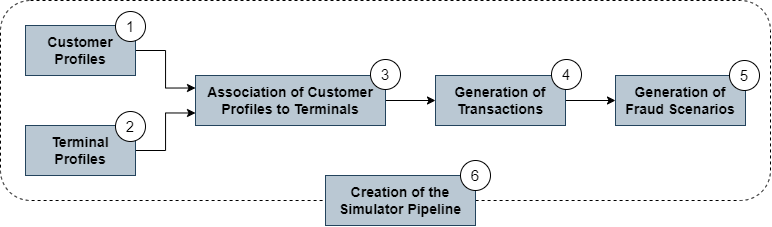
\includegraphics{images/simulator.png}
\caption{simulator}
\end{figure}

    \begin{tcolorbox}[breakable, size=fbox, boxrule=1pt, pad at break*=1mm,colback=cellbackground, colframe=cellborder]
\prompt{In}{incolor}{1}{\boxspacing}
\begin{Verbatim}[commandchars=\\\{\}]
\PY{k+kn}{import} \PY{n+nn}{os}
\PY{k+kn}{import} \PY{n+nn}{numpy} \PY{k}{as} \PY{n+nn}{np}
\PY{k+kn}{import} \PY{n+nn}{pandas} \PY{k}{as} \PY{n+nn}{pd}
\PY{k+kn}{import} \PY{n+nn}{datetime}
\PY{k+kn}{import} \PY{n+nn}{time}
\PY{k+kn}{import} \PY{n+nn}{random}
\PY{k+kn}{import} \PY{n+nn}{matplotlib}\PY{n+nn}{.}\PY{n+nn}{pyplot} \PY{k}{as} \PY{n+nn}{plt}
\PY{k+kn}{import} \PY{n+nn}{seaborn} \PY{k}{as} \PY{n+nn}{sns}
\PY{k+kn}{from} \PY{n+nn}{neo4j} \PY{k+kn}{import} \PY{n}{GraphDatabase}
\PY{k+kn}{from} \PY{n+nn}{tqdm}\PY{n+nn}{.}\PY{n+nn}{notebook} \PY{k+kn}{import} \PY{n}{tqdm}
\PY{k+kn}{import} \PY{n+nn}{warnings}

\PY{o}{\PYZpc{}}\PY{k}{matplotlib} inline
\PY{n}{pd}\PY{o}{.}\PY{n}{set\PYZus{}option}\PY{p}{(}\PY{l+s+s1}{\PYZsq{}}\PY{l+s+s1}{display.notebook\PYZus{}repr\PYZus{}html}\PY{l+s+s1}{\PYZsq{}}\PY{p}{,} \PY{k+kc}{True}\PY{p}{)}
\PY{n}{pd}\PY{o}{.}\PY{n}{DataFrame}\PY{o}{.}\PY{n}{\PYZus{}repr\PYZus{}latex\PYZus{}} \PY{o}{=} \PY{k}{lambda} \PY{n+nb+bp}{self}\PY{p}{:} \PY{l+s+s2}{\PYZdq{}}\PY{l+s+se}{\PYZbs{}n}\PY{l+s+s2}{\PYZdq{}}\PY{o}{.}\PY{n}{join}\PY{p}{(}\PY{p}{[}\PY{l+s+sa}{r}\PY{l+s+s1}{\PYZsq{}}\PY{l+s+s1}{\PYZbs{}}\PY{l+s+s1}{begin}\PY{l+s+si}{\PYZob{}center\PYZcb{}}\PY{l+s+s1}{\PYZsq{}}\PY{p}{,} \PY{n+nb+bp}{self}\PY{o}{.}\PY{n}{to\PYZus{}latex}\PY{p}{(}\PY{p}{)}\PY{p}{,} \PY{l+s+sa}{r}\PY{l+s+s1}{\PYZsq{}}\PY{l+s+s1}{\PYZbs{}}\PY{l+s+s1}{end}\PY{l+s+si}{\PYZob{}center\PYZcb{}}\PY{l+s+s1}{\PYZsq{}}\PY{p}{]}\PY{p}{)}
\PY{n}{sns}\PY{o}{.}\PY{n}{set\PYZus{}style}\PY{p}{(}\PY{l+s+s1}{\PYZsq{}}\PY{l+s+s1}{darkgrid}\PY{l+s+s1}{\PYZsq{}}\PY{p}{,} \PY{p}{\PYZob{}}\PY{l+s+s1}{\PYZsq{}}\PY{l+s+s1}{axes.facecolor}\PY{l+s+s1}{\PYZsq{}}\PY{p}{:} \PY{l+s+s1}{\PYZsq{}}\PY{l+s+s1}{0.9}\PY{l+s+s1}{\PYZsq{}}\PY{p}{\PYZcb{}}\PY{p}{)}
\PY{n}{warnings}\PY{o}{.}\PY{n}{filterwarnings}\PY{p}{(}\PY{l+s+s1}{\PYZsq{}}\PY{l+s+s1}{ignore}\PY{l+s+s1}{\PYZsq{}}\PY{p}{)}
\end{Verbatim}
\end{tcolorbox}

    \hypertarget{customer-profiles-generation}{%
\subsection{Customer Profiles
Generation}\label{customer-profiles-generation}}

    Unique spending habits are simulated through customer attributes such as
location, spending frequency, and spending amount, organized into
\texttt{customer\_profiles\_table}. Each customer is characterized by:

\begin{itemize}
\tightlist
\item
  \texttt{CUSTOMER\_ID}: A unique identifier for the customer.
\item
  \texttt{(x\_customer\_id,\ y\_customer\_id)}: Real coordinates
  representing the customer's geographical location on a 100 * 100 grid.
\item
  \texttt{(mean\_amount,\ std\_amount)}: The mean and standard deviation
  of transaction amounts for the customer
\item
  \texttt{mean\_nb\_tx\_per\_day}: The average number of transactions
  per day for the customer
\end{itemize}

    \begin{tcolorbox}[breakable, size=fbox, boxrule=1pt, pad at break*=1mm,colback=cellbackground, colframe=cellborder]
\prompt{In}{incolor}{2}{\boxspacing}
\begin{Verbatim}[commandchars=\\\{\}]
\PY{k}{def} \PY{n+nf}{generate\PYZus{}customer\PYZus{}profiles\PYZus{}table}\PY{p}{(}\PY{n}{n\PYZus{}customers}\PY{p}{,} \PY{n}{random\PYZus{}state}\PY{o}{=}\PY{l+m+mi}{0}\PY{p}{)}\PY{p}{:}
\PY{+w}{    }\PY{l+s+sd}{\PYZsq{}\PYZsq{}\PYZsq{}}
\PY{l+s+sd}{    This function provides an implementation for generating a table of customer}
\PY{l+s+sd}{    profiles. It takes as input the number of customers for which to generate a}
\PY{l+s+sd}{    profile and a random state for reproducibility. It returns a DataFrame}
\PY{l+s+sd}{    containing the properties for each customer.}
\PY{l+s+sd}{    \PYZsq{}\PYZsq{}\PYZsq{}}
    \PY{n}{np}\PY{o}{.}\PY{n}{random}\PY{o}{.}\PY{n}{seed}\PY{p}{(}\PY{n}{random\PYZus{}state}\PY{p}{)}
    \PY{n}{customer\PYZus{}id\PYZus{}properties}\PY{o}{=}\PY{p}{[}\PY{p}{]}

    \PY{c+c1}{\PYZsh{} Generate customer properties from random distributions}
    \PY{k}{for} \PY{n}{customer\PYZus{}id} \PY{o+ow}{in} \PY{n+nb}{range}\PY{p}{(}\PY{n}{n\PYZus{}customers}\PY{p}{)}\PY{p}{:}
        \PY{n}{x\PYZus{}customer\PYZus{}id} \PY{o}{=} \PY{n}{np}\PY{o}{.}\PY{n}{random}\PY{o}{.}\PY{n}{uniform}\PY{p}{(}\PY{l+m+mi}{0}\PY{p}{,}\PY{l+m+mi}{100}\PY{p}{)}
        \PY{n}{y\PYZus{}customer\PYZus{}id} \PY{o}{=} \PY{n}{np}\PY{o}{.}\PY{n}{random}\PY{o}{.}\PY{n}{uniform}\PY{p}{(}\PY{l+m+mi}{0}\PY{p}{,}\PY{l+m+mi}{100}\PY{p}{)}
        \PY{c+c1}{\PYZsh{} Arbitrary (but sensible) values}
        \PY{n}{mean\PYZus{}amount} \PY{o}{=} \PY{n}{np}\PY{o}{.}\PY{n}{random}\PY{o}{.}\PY{n}{uniform}\PY{p}{(}\PY{l+m+mi}{5}\PY{p}{,}\PY{l+m+mi}{100}\PY{p}{)}
        \PY{n}{std\PYZus{}amount} \PY{o}{=} \PY{n}{mean\PYZus{}amount}\PY{o}{/}\PY{l+m+mi}{2}
        \PY{n}{mean\PYZus{}nb\PYZus{}tx\PYZus{}per\PYZus{}day} \PY{o}{=} \PY{n}{np}\PY{o}{.}\PY{n}{random}\PY{o}{.}\PY{n}{uniform}\PY{p}{(}\PY{l+m+mi}{0}\PY{p}{,}\PY{l+m+mi}{4}\PY{p}{)}
        \PY{n}{customer\PYZus{}id\PYZus{}properties}\PY{o}{.}\PY{n}{append}\PY{p}{(}\PY{p}{[}\PY{n}{customer\PYZus{}id}\PY{p}{,}
                                      \PY{n}{x\PYZus{}customer\PYZus{}id}\PY{p}{,} \PY{n}{y\PYZus{}customer\PYZus{}id}\PY{p}{,}
                                      \PY{n}{mean\PYZus{}amount}\PY{p}{,} \PY{n}{std\PYZus{}amount}\PY{p}{,}
                                      \PY{n}{mean\PYZus{}nb\PYZus{}tx\PYZus{}per\PYZus{}day}\PY{p}{]}\PY{p}{)}

    \PY{n}{customer\PYZus{}profiles\PYZus{}table} \PY{o}{=} \PY{n}{pd}\PY{o}{.}\PY{n}{DataFrame}\PY{p}{(}\PY{n}{customer\PYZus{}id\PYZus{}properties}\PY{p}{,} \PY{n}{columns}\PY{o}{=} \PY{p}{[}
            \PY{l+s+s1}{\PYZsq{}}\PY{l+s+s1}{CUSTOMER\PYZus{}ID}\PY{l+s+s1}{\PYZsq{}}\PY{p}{,}
            \PY{l+s+s1}{\PYZsq{}}\PY{l+s+s1}{x\PYZus{}customer\PYZus{}id}\PY{l+s+s1}{\PYZsq{}}\PY{p}{,} \PY{l+s+s1}{\PYZsq{}}\PY{l+s+s1}{y\PYZus{}customer\PYZus{}id}\PY{l+s+s1}{\PYZsq{}}\PY{p}{,}
            \PY{l+s+s1}{\PYZsq{}}\PY{l+s+s1}{mean\PYZus{}amount}\PY{l+s+s1}{\PYZsq{}}\PY{p}{,} \PY{l+s+s1}{\PYZsq{}}\PY{l+s+s1}{std\PYZus{}amount}\PY{l+s+s1}{\PYZsq{}}\PY{p}{,}
            \PY{l+s+s1}{\PYZsq{}}\PY{l+s+s1}{mean\PYZus{}nb\PYZus{}tx\PYZus{}per\PYZus{}day}\PY{l+s+s1}{\PYZsq{}}\PY{p}{]}\PY{p}{)}
    \PY{k}{return} \PY{n}{customer\PYZus{}profiles\PYZus{}table}
\end{Verbatim}
\end{tcolorbox}

    \begin{tcolorbox}[breakable, size=fbox, boxrule=1pt, pad at break*=1mm,colback=cellbackground, colframe=cellborder]
\prompt{In}{incolor}{3}{\boxspacing}
\begin{Verbatim}[commandchars=\\\{\}]
\PY{n}{customer\PYZus{}profiles\PYZus{}table} \PY{o}{=} \PY{n}{generate\PYZus{}customer\PYZus{}profiles\PYZus{}table}\PY{p}{(}\PY{n}{n\PYZus{}customers}\PY{o}{=}\PY{l+m+mi}{5}\PY{p}{)}
\PY{n}{customer\PYZus{}profiles\PYZus{}table}\PY{o}{.}\PY{n}{rename}\PY{p}{(}\PY{n}{columns}\PY{o}{=}\PY{k}{lambda} \PY{n}{x}\PY{p}{:} \PY{n}{x}\PY{o}{.}\PY{n}{replace}\PY{p}{(}\PY{l+s+s1}{\PYZsq{}}\PY{l+s+s1}{\PYZus{}}\PY{l+s+s1}{\PYZsq{}}\PY{p}{,} \PY{l+s+s1}{\PYZsq{}}\PY{l+s+s1}{\PYZhy{}}\PY{l+s+s1}{\PYZsq{}}\PY{p}{)}\PY{p}{)}
\end{Verbatim}
\end{tcolorbox}
 
            
\prompt{Out}{outcolor}{3}{}
    
    \begin{center}
\begin{tabular}{lrrrrrr}
\toprule
 & CUSTOMER-ID & x-customer-id & y-customer-id & mean-amount & std-amount & mean-nb-tx-per-day \\
\midrule
0 & 0 & 54.881350 & 71.518937 & 62.262521 & 31.131260 & 2.179533 \\
1 & 1 & 42.365480 & 64.589411 & 46.570785 & 23.285393 & 3.567092 \\
2 & 2 & 96.366276 & 38.344152 & 80.213879 & 40.106939 & 2.115580 \\
3 & 3 & 56.804456 & 92.559664 & 11.748426 & 5.874213 & 0.348517 \\
4 & 4 & 2.021840 & 83.261985 & 78.924891 & 39.462446 & 3.480049 \\
\bottomrule
\end{tabular}

\end{center}

    

    \hypertarget{terminal-profiles-generation}{%
\subsection{Terminal Profiles
Generation}\label{terminal-profiles-generation}}

    Terminal characteristics represented in
\texttt{terminal\_profiles\_table}, focus solely on geographical
location. Each terminal will be defined by the following properties:

\begin{itemize}
\tightlist
\item
  \texttt{TERMINAL\_ID}: The terminal ID
\item
  \texttt{(x\_terminal\_id,\ y\_terminal\_id)}: A pair of real
  coordinates defining the geographical location of the terminal
\end{itemize}

    \begin{tcolorbox}[breakable, size=fbox, boxrule=1pt, pad at break*=1mm,colback=cellbackground, colframe=cellborder]
\prompt{In}{incolor}{4}{\boxspacing}
\begin{Verbatim}[commandchars=\\\{\}]
\PY{k}{def} \PY{n+nf}{generate\PYZus{}terminal\PYZus{}profiles\PYZus{}table}\PY{p}{(}\PY{n}{n\PYZus{}terminals}\PY{p}{,} \PY{n}{random\PYZus{}state}\PY{o}{=}\PY{l+m+mi}{0}\PY{p}{)}\PY{p}{:}
\PY{+w}{    }\PY{l+s+sd}{\PYZsq{}\PYZsq{}\PYZsq{}}
\PY{l+s+sd}{    This function provides an implementation for generating a table of terminal}
\PY{l+s+sd}{    profiles. It takes as input the number of terminals for which to generate a}
\PY{l+s+sd}{    profile and a random state for reproducibility. It returns a DataFrame}
\PY{l+s+sd}{    containing the properties for each terminal.}
\PY{l+s+sd}{    \PYZsq{}\PYZsq{}\PYZsq{}}

    \PY{n}{np}\PY{o}{.}\PY{n}{random}\PY{o}{.}\PY{n}{seed}\PY{p}{(}\PY{n}{random\PYZus{}state}\PY{p}{)}
    \PY{n}{terminal\PYZus{}id\PYZus{}properties}\PY{o}{=}\PY{p}{[}\PY{p}{]}
    \PY{c+c1}{\PYZsh{} Generate terminal properties from random distributions}
    \PY{k}{for} \PY{n}{terminal\PYZus{}id} \PY{o+ow}{in} \PY{n+nb}{range}\PY{p}{(}\PY{n}{n\PYZus{}terminals}\PY{p}{)}\PY{p}{:}
        \PY{n}{x\PYZus{}terminal\PYZus{}id} \PY{o}{=} \PY{n}{np}\PY{o}{.}\PY{n}{random}\PY{o}{.}\PY{n}{uniform}\PY{p}{(}\PY{l+m+mi}{0}\PY{p}{,}\PY{l+m+mi}{100}\PY{p}{)}
        \PY{n}{y\PYZus{}terminal\PYZus{}id} \PY{o}{=} \PY{n}{np}\PY{o}{.}\PY{n}{random}\PY{o}{.}\PY{n}{uniform}\PY{p}{(}\PY{l+m+mi}{0}\PY{p}{,}\PY{l+m+mi}{100}\PY{p}{)}
        \PY{n}{terminal\PYZus{}id\PYZus{}properties}\PY{o}{.}\PY{n}{append}\PY{p}{(}\PY{p}{[}\PY{n}{terminal\PYZus{}id}\PY{p}{,}
                                      \PY{n}{x\PYZus{}terminal\PYZus{}id}\PY{p}{,} \PY{n}{y\PYZus{}terminal\PYZus{}id}\PY{p}{]}\PY{p}{)}

    \PY{n}{terminal\PYZus{}profiles\PYZus{}table} \PY{o}{=} \PY{n}{pd}\PY{o}{.}\PY{n}{DataFrame}\PY{p}{(}\PY{n}{terminal\PYZus{}id\PYZus{}properties}\PY{p}{,} \PY{n}{columns}\PY{o}{=}
        \PY{p}{[}\PY{l+s+s1}{\PYZsq{}}\PY{l+s+s1}{TERMINAL\PYZus{}ID}\PY{l+s+s1}{\PYZsq{}}\PY{p}{,} \PY{l+s+s1}{\PYZsq{}}\PY{l+s+s1}{x\PYZus{}terminal\PYZus{}id}\PY{l+s+s1}{\PYZsq{}}\PY{p}{,} \PY{l+s+s1}{\PYZsq{}}\PY{l+s+s1}{y\PYZus{}terminal\PYZus{}id}\PY{l+s+s1}{\PYZsq{}}\PY{p}{]}\PY{p}{)}
    \PY{k}{return} \PY{n}{terminal\PYZus{}profiles\PYZus{}table}
\end{Verbatim}
\end{tcolorbox}

    \begin{tcolorbox}[breakable, size=fbox, boxrule=1pt, pad at break*=1mm,colback=cellbackground, colframe=cellborder]
\prompt{In}{incolor}{5}{\boxspacing}
\begin{Verbatim}[commandchars=\\\{\}]
\PY{n}{terminal\PYZus{}profiles\PYZus{}table} \PY{o}{=} \PY{n}{generate\PYZus{}terminal\PYZus{}profiles\PYZus{}table}\PY{p}{(}\PY{n}{n\PYZus{}terminals}\PY{o}{=}\PY{l+m+mi}{5}\PY{p}{)}
\PY{n}{terminal\PYZus{}profiles\PYZus{}table}\PY{o}{.}\PY{n}{rename}\PY{p}{(}\PY{n}{columns}\PY{o}{=}\PY{k}{lambda} \PY{n}{x}\PY{p}{:} \PY{n}{x}\PY{o}{.}\PY{n}{replace}\PY{p}{(}\PY{l+s+s1}{\PYZsq{}}\PY{l+s+s1}{\PYZus{}}\PY{l+s+s1}{\PYZsq{}}\PY{p}{,} \PY{l+s+s1}{\PYZsq{}}\PY{l+s+s1}{\PYZhy{}}\PY{l+s+s1}{\PYZsq{}}\PY{p}{)}\PY{p}{)}
\end{Verbatim}
\end{tcolorbox}
 
            
\prompt{Out}{outcolor}{5}{}
    
    \begin{center}
\begin{tabular}{lrrr}
\toprule
 & TERMINAL-ID & x-terminal-id & y-terminal-id \\
\midrule
0 & 0 & 54.881350 & 71.518937 \\
1 & 1 & 60.276338 & 54.488318 \\
2 & 2 & 42.365480 & 64.589411 \\
3 & 3 & 43.758721 & 89.177300 \\
4 & 4 & 96.366276 & 38.344152 \\
\bottomrule
\end{tabular}

\end{center}

    

    \hypertarget{association-of-customer-profiles-to-terminals}{%
\subsection{Association of Customer Profiles to
Terminals}\label{association-of-customer-profiles-to-terminals}}

    Customers are assumed to transact only at terminals within a certain
radius \texttt{r} of their geographical location, reflected in the
\texttt{available\_terminals} feature added to each customer profile.
Comparing the terminal locations stored in
\texttt{terminal\_profiles\_table} and the customer locations in
\texttt{customer\_profiles\_table}, we can compute the list of available
terminals for a given customer at a given radius. The plot below
demonstrates how the radius can affect the inclusion of surrounding
terminals.

\begin{figure}
\centering
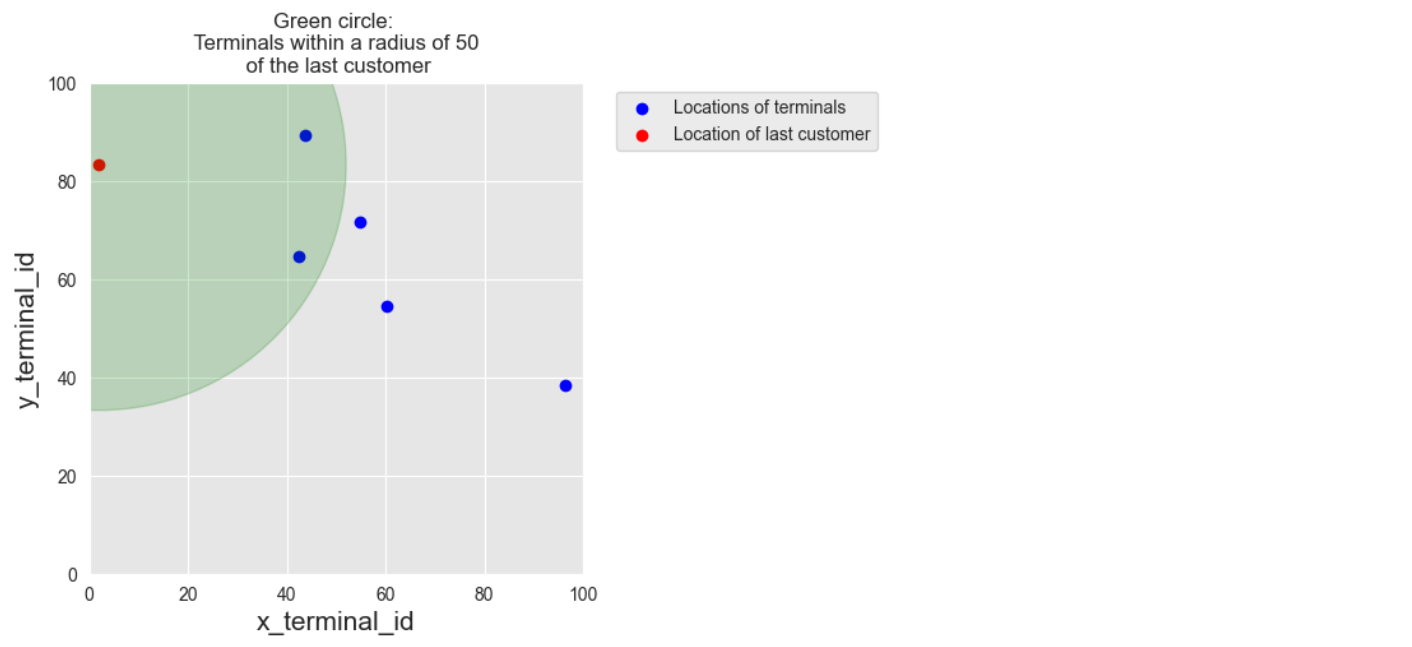
\includegraphics{images/available_terminals.png}
\caption{available\_terminals}
\end{figure}

    \begin{tcolorbox}[breakable, size=fbox, boxrule=1pt, pad at break*=1mm,colback=cellbackground, colframe=cellborder]
\prompt{In}{incolor}{6}{\boxspacing}
\begin{Verbatim}[commandchars=\\\{\}]
\PY{k}{def} \PY{n+nf}{get\PYZus{}list\PYZus{}terminals\PYZus{}within\PYZus{}radius}\PY{p}{(}\PY{n}{customer\PYZus{}profile}\PY{p}{,} \PY{n}{x\PYZus{}y\PYZus{}terminals}\PY{p}{,} \PY{n}{r}\PY{p}{)}\PY{p}{:}
\PY{+w}{    }\PY{l+s+sd}{\PYZsq{}\PYZsq{}\PYZsq{}}
\PY{l+s+sd}{    This function returns the list of terminals within a radius of r, given as}
\PY{l+s+sd}{    input a customer profile (any row in the customer profiles table), an array}
\PY{l+s+sd}{    containing the geographical location of all terminals, and the radius r.}
\PY{l+s+sd}{    \PYZsq{}\PYZsq{}\PYZsq{}}
    \PY{c+c1}{\PYZsh{} Location (x,y) of customer as numpy array}
    \PY{n}{x\PYZus{}y\PYZus{}customer} \PY{o}{=} \PY{n}{customer\PYZus{}profile}\PY{p}{[}\PY{p}{[}\PY{l+s+s1}{\PYZsq{}}\PY{l+s+s1}{x\PYZus{}customer\PYZus{}id}\PY{l+s+s1}{\PYZsq{}}\PY{p}{,}\PY{l+s+s1}{\PYZsq{}}\PY{l+s+s1}{y\PYZus{}customer\PYZus{}id}\PY{l+s+s1}{\PYZsq{}}\PY{p}{]}\PY{p}{]}\PY{o}{.}\PY{n}{values}\PY{o}{.}\PY{n}{astype}\PY{p}{(}\PY{n+nb}{float}\PY{p}{)}

    \PY{c+c1}{\PYZsh{} Squared difference in coordinates between customer and terminal locations}
    \PY{n}{squared\PYZus{}diff\PYZus{}x\PYZus{}y} \PY{o}{=} \PY{n}{np}\PY{o}{.}\PY{n}{square}\PY{p}{(}\PY{n}{x\PYZus{}y\PYZus{}customer} \PY{o}{\PYZhy{}} \PY{n}{x\PYZus{}y\PYZus{}terminals}\PY{p}{)}

    \PY{c+c1}{\PYZsh{} Sum along rows and compute suared root to get distance}
    \PY{n}{dist\PYZus{}x\PYZus{}y} \PY{o}{=} \PY{n}{np}\PY{o}{.}\PY{n}{sqrt}\PY{p}{(}\PY{n}{np}\PY{o}{.}\PY{n}{sum}\PY{p}{(}\PY{n}{squared\PYZus{}diff\PYZus{}x\PYZus{}y}\PY{p}{,} \PY{n}{axis}\PY{o}{=}\PY{l+m+mi}{1}\PY{p}{)}\PY{p}{)}

    \PY{c+c1}{\PYZsh{} Get the indices of terminals which are at a distance less than r}
    \PY{n}{available\PYZus{}terminals} \PY{o}{=} \PY{n+nb}{list}\PY{p}{(}\PY{n}{np}\PY{o}{.}\PY{n}{where}\PY{p}{(}\PY{n}{dist\PYZus{}x\PYZus{}y}\PY{o}{\PYZlt{}}\PY{n}{r}\PY{p}{)}\PY{p}{[}\PY{l+m+mi}{0}\PY{p}{]}\PY{p}{)}

    \PY{c+c1}{\PYZsh{} Return the list of terminal IDs}
    \PY{k}{return} \PY{n}{available\PYZus{}terminals}
\end{Verbatim}
\end{tcolorbox}

    Calculating the available terminals for each customer can be performed
using the pandas \texttt{apply} function. The results are stored as a
new column named \texttt{available\_terminals} in the customer profiles
table.

    \begin{tcolorbox}[breakable, size=fbox, boxrule=1pt, pad at break*=1mm,colback=cellbackground, colframe=cellborder]
\prompt{In}{incolor}{7}{\boxspacing}
\begin{Verbatim}[commandchars=\\\{\}]
\PY{c+c1}{\PYZsh{} We first get the geographical locations of all terminals as a numpy array}
\PY{n}{x\PYZus{}y\PYZus{}terminals} \PY{o}{=} \PY{n}{terminal\PYZus{}profiles\PYZus{}table}\PY{p}{[}\PY{p}{[}\PY{l+s+s1}{\PYZsq{}}\PY{l+s+s1}{x\PYZus{}terminal\PYZus{}id}\PY{l+s+s1}{\PYZsq{}}\PY{p}{,}\PY{l+s+s1}{\PYZsq{}}\PY{l+s+s1}{y\PYZus{}terminal\PYZus{}id}\PY{l+s+s1}{\PYZsq{}}\PY{p}{]}\PY{p}{]}\PY{o}{.}\PY{n}{values}\PY{o}{.}\PY{n}{astype}\PY{p}{(}\PY{n+nb}{float}\PY{p}{)}

\PY{c+c1}{\PYZsh{} Now we compute the available terminals}
\PY{n}{customer\PYZus{}profiles\PYZus{}table}\PY{p}{[}\PY{l+s+s1}{\PYZsq{}}\PY{l+s+s1}{available\PYZus{}terminals}\PY{l+s+s1}{\PYZsq{}}\PY{p}{]} \PY{o}{=} \PYZbs{}
    \PY{n}{customer\PYZus{}profiles\PYZus{}table}\PY{o}{.}\PY{n}{apply}\PY{p}{(}\PY{k}{lambda} \PY{n}{x} \PY{p}{:} \PYZbs{}
        \PY{n}{get\PYZus{}list\PYZus{}terminals\PYZus{}within\PYZus{}radius}\PY{p}{(}\PY{n}{x}\PY{p}{,} \PY{n}{x\PYZus{}y\PYZus{}terminals}\PY{o}{=}\PY{n}{x\PYZus{}y\PYZus{}terminals}\PY{p}{,} \PY{n}{r}\PY{o}{=}\PY{l+m+mi}{50}\PY{p}{)}\PY{p}{,}
        \PY{n}{axis}\PY{o}{=}\PY{l+m+mi}{1}
    \PY{p}{)}
\PY{n}{customer\PYZus{}profiles\PYZus{}table}\PY{o}{.}\PY{n}{rename}\PY{p}{(}\PY{n}{columns}\PY{o}{=}\PY{k}{lambda} \PY{n}{x}\PY{p}{:} \PY{n}{x}\PY{o}{.}\PY{n}{replace}\PY{p}{(}\PY{l+s+s1}{\PYZsq{}}\PY{l+s+s1}{\PYZus{}}\PY{l+s+s1}{\PYZsq{}}\PY{p}{,} \PY{l+s+s1}{\PYZsq{}}\PY{l+s+s1}{\PYZhy{}}\PY{l+s+s1}{\PYZsq{}}\PY{p}{)}\PY{p}{)}
\end{Verbatim}
\end{tcolorbox}
 
            
\prompt{Out}{outcolor}{7}{}
    
    \begin{center}
\footnotesize
\begin{tabular}{lrrrrrrl}
\toprule
 & CUSTOMER-ID & x-customer-id & y-customer-id & mean-amount & std-amount & mean-nb-tx-per-day & available-terminals \\
\midrule
0 & 0 & 54.881350 & 71.518937 & 62.262521 & 31.131260 & 2.179533 & [0, 1, 2, 3] \\
1 & 1 & 42.365480 & 64.589411 & 46.570785 & 23.285393 & 3.567092 & [0, 1, 2, 3] \\
2 & 2 & 96.366276 & 38.344152 & 80.213879 & 40.106939 & 2.115580 & [1, 4] \\
3 & 3 & 56.804456 & 92.559664 & 11.748426 & 5.874213 & 0.348517 & [0, 1, 2, 3] \\
4 & 4 & 2.021840 & 83.261985 & 78.924891 & 39.462446 & 3.480049 & [2, 3] \\
\bottomrule
\end{tabular}

\end{center}

    

    \hypertarget{generation-of-transactions}{%
\subsection{Generation of
Transactions}\label{generation-of-transactions}}

    Transactions are generated based on customer attributes and terminal
availability, resulting in a \texttt{transactions\_df} table. We have
now all the necessary information to generate the transactions, using
the \texttt{generate\_transactions\_table} function below. This function
will attempt to randomly populate the transaction data starting from a
given date, until a certain number of days. Most of the values will be
generated randomly, yet following a normal, uniform, or Poisson
distribution. We can verify that the generated transactions comply with
the customer profile properties:

\begin{itemize}
\tightlist
\item
  The \texttt{TERMINAL\_ID}s correspond to those in the list of
  available terminals. However, not necessarily all these available
  terminals will be selected. As a result, the
  \texttt{available\_terminals} is NOT equivalent to the actual
  terminals to which each customer is connected.
\item
  The \texttt{TX\_AMOUNT}s appear to align with the customer's amount
  parameters represented as \texttt{mean\_amount} and
  \texttt{std\_amount}.
\item
  The number of transactions per day varies based on the transaction
  frequency parameters of the customer,
  i.e.~\texttt{mean\_nb\_tx\_per\_day}.
\end{itemize}

    \begin{tcolorbox}[breakable, size=fbox, boxrule=1pt, pad at break*=1mm,colback=cellbackground, colframe=cellborder]
\prompt{In}{incolor}{8}{\boxspacing}
\begin{Verbatim}[commandchars=\\\{\}]
\PY{k}{def} \PY{n+nf}{generate\PYZus{}transactions\PYZus{}table}\PY{p}{(}\PY{n}{customer\PYZus{}profile}\PY{p}{,} \PY{n}{start\PYZus{}date} \PY{o}{=} \PY{l+s+s2}{\PYZdq{}}\PY{l+s+s2}{2018\PYZhy{}04\PYZhy{}01}\PY{l+s+s2}{\PYZdq{}}\PY{p}{,} \PY{n}{nb\PYZus{}days} \PY{o}{=} \PY{l+m+mi}{10}\PY{p}{)}\PY{p}{:}
\PY{+w}{    }\PY{l+s+sd}{\PYZsq{}\PYZsq{}\PYZsq{}}
\PY{l+s+sd}{    takes as input a customer profile, a starting date, and a number of days for}
\PY{l+s+sd}{    which to generate transactions. It will return a table of transactions}
\PY{l+s+sd}{    without considering the labels}
\PY{l+s+sd}{    \PYZsq{}\PYZsq{}\PYZsq{}}
    \PY{n}{customer\PYZus{}transactions} \PY{o}{=} \PY{p}{[}\PY{p}{]}
    \PY{n}{random}\PY{o}{.}\PY{n}{seed}\PY{p}{(}\PY{n+nb}{int}\PY{p}{(}\PY{n}{customer\PYZus{}profile}\PY{o}{.}\PY{n}{CUSTOMER\PYZus{}ID}\PY{p}{)}\PY{p}{)}
    \PY{n}{np}\PY{o}{.}\PY{n}{random}\PY{o}{.}\PY{n}{seed}\PY{p}{(}\PY{n+nb}{int}\PY{p}{(}\PY{n}{customer\PYZus{}profile}\PY{o}{.}\PY{n}{CUSTOMER\PYZus{}ID}\PY{p}{)}\PY{p}{)}

    \PY{c+c1}{\PYZsh{} For all days}
    \PY{k}{for} \PY{n}{day} \PY{o+ow}{in} \PY{n+nb}{range}\PY{p}{(}\PY{n}{nb\PYZus{}days}\PY{p}{)}\PY{p}{:}
        \PY{c+c1}{\PYZsh{} Random number of transactions for that day}
        \PY{n}{nb\PYZus{}tx} \PY{o}{=} \PY{n}{np}\PY{o}{.}\PY{n}{random}\PY{o}{.}\PY{n}{poisson}\PY{p}{(}\PY{n}{customer\PYZus{}profile}\PY{o}{.}\PY{n}{mean\PYZus{}nb\PYZus{}tx\PYZus{}per\PYZus{}day}\PY{p}{)}
        \PY{c+c1}{\PYZsh{} If nb\PYZus{}tx positive, let us generate transactions}
        \PY{k}{if} \PY{n}{nb\PYZus{}tx}\PY{o}{\PYZgt{}}\PY{l+m+mi}{0}\PY{p}{:}
            \PY{k}{for} \PY{n}{tx} \PY{o+ow}{in} \PY{n+nb}{range}\PY{p}{(}\PY{n}{nb\PYZus{}tx}\PY{p}{)}\PY{p}{:}
                \PY{c+c1}{\PYZsh{} Time of transaction: Around noon, std 20000 seconds. This choice aims at simulating the fact that}
                \PY{c+c1}{\PYZsh{} most transactions occur during the day.}
                \PY{n}{time\PYZus{}tx} \PY{o}{=} \PY{n+nb}{int}\PY{p}{(}\PY{n}{np}\PY{o}{.}\PY{n}{random}\PY{o}{.}\PY{n}{normal}\PY{p}{(}\PY{l+m+mi}{86400}\PY{o}{/}\PY{l+m+mi}{2}\PY{p}{,} \PY{l+m+mi}{20000}\PY{p}{)}\PY{p}{)}

                \PY{c+c1}{\PYZsh{} If transaction time between 0 and 86400, let us keep it, otherwise, let us discard it}
                \PY{k}{if} \PY{p}{(}\PY{n}{time\PYZus{}tx}\PY{o}{\PYZgt{}}\PY{l+m+mi}{0}\PY{p}{)} \PY{o+ow}{and} \PY{p}{(}\PY{n}{time\PYZus{}tx}\PY{o}{\PYZlt{}}\PY{l+m+mi}{86400}\PY{p}{)}\PY{p}{:}
                    \PY{c+c1}{\PYZsh{} Amount is drawn from a normal distribution}
                    \PY{n}{amount} \PY{o}{=} \PY{n}{np}\PY{o}{.}\PY{n}{random}\PY{o}{.}\PY{n}{normal}\PY{p}{(}\PY{n}{customer\PYZus{}profile}\PY{o}{.}\PY{n}{mean\PYZus{}amount}\PY{p}{,} \PY{n}{customer\PYZus{}profile}\PY{o}{.}\PY{n}{std\PYZus{}amount}\PY{p}{)}
                    \PY{c+c1}{\PYZsh{} If amount negative, draw from a uniform distribution}
                    \PY{k}{if} \PY{n}{amount}\PY{o}{\PYZlt{}}\PY{l+m+mi}{0}\PY{p}{:}
                        \PY{n}{amount} \PY{o}{=} \PY{n}{np}\PY{o}{.}\PY{n}{random}\PY{o}{.}\PY{n}{uniform}\PY{p}{(}\PY{l+m+mi}{0}\PY{p}{,}\PY{n}{customer\PYZus{}profile}\PY{o}{.}\PY{n}{mean\PYZus{}amount}\PY{o}{*}\PY{l+m+mi}{2}\PY{p}{)}

                    \PY{n}{amount}\PY{o}{=}\PY{n}{np}\PY{o}{.}\PY{n}{round}\PY{p}{(}\PY{n}{amount}\PY{p}{,}\PY{n}{decimals}\PY{o}{=}\PY{l+m+mi}{2}\PY{p}{)}
                    \PY{k}{if} \PY{n+nb}{len}\PY{p}{(}\PY{n}{customer\PYZus{}profile}\PY{o}{.}\PY{n}{available\PYZus{}terminals}\PY{p}{)}\PY{o}{\PYZgt{}}\PY{l+m+mi}{0}\PY{p}{:}
                        \PY{n}{terminal\PYZus{}id} \PY{o}{=} \PY{n}{random}\PY{o}{.}\PY{n}{choice}\PY{p}{(}\PY{n}{customer\PYZus{}profile}\PY{o}{.}\PY{n}{available\PYZus{}terminals}\PY{p}{)}
                        \PY{n}{customer\PYZus{}transactions}\PY{o}{.}\PY{n}{append}\PY{p}{(}\PY{p}{[}\PY{n}{time\PYZus{}tx}\PY{o}{+}\PY{n}{day}\PY{o}{*}\PY{l+m+mi}{86400}\PY{p}{,} \PY{n}{day}\PY{p}{,}
                                                      \PY{n}{customer\PYZus{}profile}\PY{o}{.}\PY{n}{CUSTOMER\PYZus{}ID}\PY{p}{,}
                                                      \PY{n}{terminal\PYZus{}id}\PY{p}{,} \PY{n}{amount}\PY{p}{]}\PY{p}{)}

    \PY{n}{customer\PYZus{}transactions} \PY{o}{=} \PY{n}{pd}\PY{o}{.}\PY{n}{DataFrame}\PY{p}{(}\PY{n}{customer\PYZus{}transactions}\PY{p}{,} \PY{n}{columns}\PY{o}{=}\PY{p}{[}\PY{l+s+s1}{\PYZsq{}}\PY{l+s+s1}{TX\PYZus{}TIME\PYZus{}SECONDS}\PY{l+s+s1}{\PYZsq{}}\PY{p}{,} \PY{l+s+s1}{\PYZsq{}}\PY{l+s+s1}{TX\PYZus{}TIME\PYZus{}DAYS}\PY{l+s+s1}{\PYZsq{}}\PY{p}{,} \PY{l+s+s1}{\PYZsq{}}\PY{l+s+s1}{CUSTOMER\PYZus{}ID}\PY{l+s+s1}{\PYZsq{}}\PY{p}{,} \PY{l+s+s1}{\PYZsq{}}\PY{l+s+s1}{TERMINAL\PYZus{}ID}\PY{l+s+s1}{\PYZsq{}}\PY{p}{,} \PY{l+s+s1}{\PYZsq{}}\PY{l+s+s1}{TX\PYZus{}AMOUNT}\PY{l+s+s1}{\PYZsq{}}\PY{p}{]}\PY{p}{)}
    \PY{k}{if} \PY{n+nb}{len}\PY{p}{(}\PY{n}{customer\PYZus{}transactions}\PY{p}{)}\PY{o}{\PYZgt{}}\PY{l+m+mi}{0}\PY{p}{:}
        \PY{n}{customer\PYZus{}transactions}\PY{p}{[}\PY{l+s+s1}{\PYZsq{}}\PY{l+s+s1}{TX\PYZus{}DATETIME}\PY{l+s+s1}{\PYZsq{}}\PY{p}{]} \PY{o}{=} \PY{n}{pd}\PY{o}{.}\PY{n}{to\PYZus{}datetime}\PY{p}{(}\PY{n}{customer\PYZus{}transactions}\PY{p}{[}\PY{l+s+s2}{\PYZdq{}}\PY{l+s+s2}{TX\PYZus{}TIME\PYZus{}SECONDS}\PY{l+s+s2}{\PYZdq{}}\PY{p}{]}\PY{p}{,} \PY{n}{unit}\PY{o}{=}\PY{l+s+s1}{\PYZsq{}}\PY{l+s+s1}{s}\PY{l+s+s1}{\PYZsq{}}\PY{p}{,} \PY{n}{origin}\PY{o}{=}\PY{n}{start\PYZus{}date}\PY{p}{)}
        \PY{n}{customer\PYZus{}transactions}\PY{o}{=}\PY{n}{customer\PYZus{}transactions}\PY{p}{[}\PY{p}{[}\PY{l+s+s1}{\PYZsq{}}\PY{l+s+s1}{TX\PYZus{}DATETIME}\PY{l+s+s1}{\PYZsq{}}\PY{p}{,}\PY{l+s+s1}{\PYZsq{}}\PY{l+s+s1}{CUSTOMER\PYZus{}ID}\PY{l+s+s1}{\PYZsq{}}\PY{p}{,} \PY{l+s+s1}{\PYZsq{}}\PY{l+s+s1}{TERMINAL\PYZus{}ID}\PY{l+s+s1}{\PYZsq{}}\PY{p}{,} \PY{l+s+s1}{\PYZsq{}}\PY{l+s+s1}{TX\PYZus{}AMOUNT}\PY{l+s+s1}{\PYZsq{}}\PY{p}{,}\PY{l+s+s1}{\PYZsq{}}\PY{l+s+s1}{TX\PYZus{}TIME\PYZus{}SECONDS}\PY{l+s+s1}{\PYZsq{}}\PY{p}{,} \PY{l+s+s1}{\PYZsq{}}\PY{l+s+s1}{TX\PYZus{}TIME\PYZus{}DAYS}\PY{l+s+s1}{\PYZsq{}}\PY{p}{]}\PY{p}{]}
    \PY{k}{return} \PY{n}{customer\PYZus{}transactions}
\end{Verbatim}
\end{tcolorbox}

    Now, let's generate transactions for all customers, which can be done
straightforwardly using the pandas \texttt{groupby} and \texttt{apply}
methods. This results in a set of 65 transactions, involving 5
customers, 5 terminals, and spanning across 5 days.

    \begin{tcolorbox}[breakable, size=fbox, boxrule=1pt, pad at break*=1mm,colback=cellbackground, colframe=cellborder]
\prompt{In}{incolor}{9}{\boxspacing}
\begin{Verbatim}[commandchars=\\\{\}]
\PY{n}{transactions\PYZus{}df}\PY{o}{=}\PY{n}{customer\PYZus{}profiles\PYZus{}table}\PY{o}{.}\PY{n}{groupby}\PY{p}{(}\PY{l+s+s1}{\PYZsq{}}\PY{l+s+s1}{CUSTOMER\PYZus{}ID}\PY{l+s+s1}{\PYZsq{}}\PY{p}{)}\PY{o}{.}\PY{n}{apply}\PY{p}{(}\PY{k}{lambda} \PY{n}{x} \PY{p}{:} \PY{n}{generate\PYZus{}transactions\PYZus{}table}\PY{p}{(}\PY{n}{x}\PY{o}{.}\PY{n}{iloc}\PY{p}{[}\PY{l+m+mi}{0}\PY{p}{]}\PY{p}{,} \PY{n}{nb\PYZus{}days}\PY{o}{=}\PY{l+m+mi}{5}\PY{p}{)}\PY{p}{)}\PY{o}{.}\PY{n}{reset\PYZus{}index}\PY{p}{(}\PY{n}{drop}\PY{o}{=}\PY{k+kc}{True}\PY{p}{)}
\PY{n}{transactions\PYZus{}df}\PY{o}{.}\PY{n}{rename}\PY{p}{(}\PY{n}{columns}\PY{o}{=}\PY{k}{lambda} \PY{n}{x}\PY{p}{:} \PY{n}{x}\PY{o}{.}\PY{n}{replace}\PY{p}{(}\PY{l+s+s1}{\PYZsq{}}\PY{l+s+s1}{\PYZus{}}\PY{l+s+s1}{\PYZsq{}}\PY{p}{,} \PY{l+s+s1}{\PYZsq{}}\PY{l+s+s1}{\PYZhy{}}\PY{l+s+s1}{\PYZsq{}}\PY{p}{)}\PY{p}{)}\PY{o}{.}\PY{n}{head}\PY{p}{(}\PY{p}{)}
\end{Verbatim}
\end{tcolorbox}
 
            
\prompt{Out}{outcolor}{9}{}
    
    \begin{center}
\small
\begin{tabular}{llrrrrr}
\toprule
 & TX-DATETIME & CUSTOMER-ID & TERMINAL-ID & TX-AMOUNT & TX-TIME-SECONDS & TX-TIME-DAYS \\
\midrule
0 & 2018-04-01 07:19:05 & 0 & 3 & 123.590000 & 26345 & 0 \\
1 & 2018-04-01 19:02:02 & 0 & 3 & 46.510000 & 68522 & 0 \\
2 & 2018-04-01 18:00:16 & 0 & 0 & 77.340000 & 64816 & 0 \\
3 & 2018-04-02 15:13:02 & 0 & 2 & 32.350000 & 141182 & 1 \\
4 & 2018-04-02 14:05:38 & 0 & 3 & 63.300000 & 137138 & 1 \\
\bottomrule
\end{tabular}

\end{center}

    

    \hypertarget{generation-of-fraud-scenarios}{%
\subsection{Generation of Fraud
Scenarios}\label{generation-of-fraud-scenarios}}

    In the final stage of the simulation, transactions are categorized as
\emph{legitimate} or \emph{fraudulent} through the following scenarios:

\begin{itemize}
\tightlist
\item
  \textbf{Scenario 1:} Any transaction exceeding \$220 is flagged as
  fraudulent. This unrealistic scenario serves as a straightforward
  pattern for validating basic fraud detection methods.
\item
  \textbf{Scenario 2:} Each day, two terminals are randomly selected.
  Transactions made on these terminals in the subsequent 28 days are
  marked as fraudulent. This scenario simulates criminal exploitation of
  terminals, such as through phishing attacks.
\item
  \textbf{Scenario 3:} Every day, three customers are randomly chosen.
  Over the next 14 days, one-third of their transactions have their
  amounts multiplied by 5 and are labeled as fraudulent. This simulates
  card-not-present fraud, where leaked customer credentials lead to
  higher-value transactions by fraudsters. Detection of this scenario
  requires tracking customer spending habits and adapting to temporary
  compromises, similar to scenario 2.
\end{itemize}

Notably, the initial month of the generated dataset has fewer fraudulent
transactions due to scenario durations. The resulting dataset highlights
class imbalance, mixes numerical and categorical features, and includes
time-dependent fraud scenarios.

    \begin{tcolorbox}[breakable, size=fbox, boxrule=1pt, pad at break*=1mm,colback=cellbackground, colframe=cellborder]
\prompt{In}{incolor}{10}{\boxspacing}
\begin{Verbatim}[commandchars=\\\{\}]
\PY{k}{def} \PY{n+nf}{add\PYZus{}frauds}\PY{p}{(}\PY{n}{customer\PYZus{}profiles\PYZus{}table}\PY{p}{,} \PY{n}{terminal\PYZus{}profiles\PYZus{}table}\PY{p}{,} \PY{n}{transactions\PYZus{}df}\PY{p}{)}\PY{p}{:}

    \PY{n}{start\PYZus{}time}\PY{o}{=}\PY{n}{time}\PY{o}{.}\PY{n}{time}\PY{p}{(}\PY{p}{)}

    \PY{c+c1}{\PYZsh{} By default, all transactions are genuine}
    \PY{n}{transactions\PYZus{}df}\PY{p}{[}\PY{l+s+s1}{\PYZsq{}}\PY{l+s+s1}{TX\PYZus{}FRAUD}\PY{l+s+s1}{\PYZsq{}}\PY{p}{]}\PY{o}{=}\PY{l+m+mi}{0}
    \PY{n}{transactions\PYZus{}df}\PY{p}{[}\PY{l+s+s1}{\PYZsq{}}\PY{l+s+s1}{TX\PYZus{}FRAUD\PYZus{}SCENARIO}\PY{l+s+s1}{\PYZsq{}}\PY{p}{]}\PY{o}{=}\PY{l+m+mi}{0}

    \PY{c+c1}{\PYZsh{} Scenario 1}
    \PY{n}{transactions\PYZus{}df}\PY{o}{.}\PY{n}{loc}\PY{p}{[}\PY{n}{transactions\PYZus{}df}\PY{o}{.}\PY{n}{TX\PYZus{}AMOUNT}\PY{o}{\PYZgt{}}\PY{l+m+mi}{220}\PY{p}{,} \PY{l+s+s1}{\PYZsq{}}\PY{l+s+s1}{TX\PYZus{}FRAUD}\PY{l+s+s1}{\PYZsq{}}\PY{p}{]}\PY{o}{=}\PY{l+m+mi}{1}
    \PY{n}{transactions\PYZus{}df}\PY{o}{.}\PY{n}{loc}\PY{p}{[}\PY{n}{transactions\PYZus{}df}\PY{o}{.}\PY{n}{TX\PYZus{}AMOUNT}\PY{o}{\PYZgt{}}\PY{l+m+mi}{220}\PY{p}{,} \PY{l+s+s1}{\PYZsq{}}\PY{l+s+s1}{TX\PYZus{}FRAUD\PYZus{}SCENARIO}\PY{l+s+s1}{\PYZsq{}}\PY{p}{]}\PY{o}{=}\PY{l+m+mi}{1}
    \PY{n}{nb\PYZus{}frauds\PYZus{}scenario\PYZus{}1}\PY{o}{=}\PY{n}{transactions\PYZus{}df}\PY{o}{.}\PY{n}{TX\PYZus{}FRAUD}\PY{o}{.}\PY{n}{sum}\PY{p}{(}\PY{p}{)}
    \PY{n+nb}{print}\PY{p}{(}\PY{l+s+s2}{\PYZdq{}}\PY{l+s+s2}{Number of frauds from scenario 1: }\PY{l+s+s2}{\PYZdq{}}\PY{o}{+}\PY{n+nb}{str}\PY{p}{(}\PY{n}{nb\PYZus{}frauds\PYZus{}scenario\PYZus{}1}\PY{p}{)}\PY{p}{)}

    \PY{c+c1}{\PYZsh{} Scenario 2}
    \PY{k}{for} \PY{n}{day} \PY{o+ow}{in} \PY{n+nb}{range}\PY{p}{(}\PY{n}{transactions\PYZus{}df}\PY{o}{.}\PY{n}{TX\PYZus{}TIME\PYZus{}DAYS}\PY{o}{.}\PY{n}{max}\PY{p}{(}\PY{p}{)}\PY{p}{)}\PY{p}{:}
        \PY{n}{compromised\PYZus{}terminals} \PY{o}{=} \PY{n}{terminal\PYZus{}profiles\PYZus{}table}\PY{o}{.}\PY{n}{TERMINAL\PYZus{}ID}\PY{o}{.}\PY{n}{sample}\PY{p}{(}\PY{n}{n}\PY{o}{=}\PY{l+m+mi}{2}\PY{p}{,} \PY{n}{random\PYZus{}state}\PY{o}{=}\PY{n}{day}\PY{p}{)}
        \PY{n}{compromised\PYZus{}transactions}\PY{o}{=}\PY{n}{transactions\PYZus{}df}\PY{p}{[}\PY{p}{(}\PY{n}{transactions\PYZus{}df}\PY{o}{.}\PY{n}{TX\PYZus{}TIME\PYZus{}DAYS}\PY{o}{\PYZgt{}}\PY{o}{=}\PY{n}{day}\PY{p}{)} \PY{o}{\PYZam{}}
                                                    \PY{p}{(}\PY{n}{transactions\PYZus{}df}\PY{o}{.}\PY{n}{TX\PYZus{}TIME\PYZus{}DAYS}\PY{o}{\PYZlt{}}\PY{n}{day}\PY{o}{+}\PY{l+m+mi}{28}\PY{p}{)} \PY{o}{\PYZam{}}
                                                    \PY{p}{(}\PY{n}{transactions\PYZus{}df}\PY{o}{.}\PY{n}{TERMINAL\PYZus{}ID}\PY{o}{.}\PY{n}{isin}\PY{p}{(}\PY{n}{compromised\PYZus{}terminals}\PY{p}{)}\PY{p}{)}\PY{p}{]}
        \PY{n}{transactions\PYZus{}df}\PY{o}{.}\PY{n}{loc}\PY{p}{[}\PY{n}{compromised\PYZus{}transactions}\PY{o}{.}\PY{n}{index}\PY{p}{,}\PY{l+s+s1}{\PYZsq{}}\PY{l+s+s1}{TX\PYZus{}FRAUD}\PY{l+s+s1}{\PYZsq{}}\PY{p}{]}\PY{o}{=}\PY{l+m+mi}{1}
        \PY{n}{transactions\PYZus{}df}\PY{o}{.}\PY{n}{loc}\PY{p}{[}\PY{n}{compromised\PYZus{}transactions}\PY{o}{.}\PY{n}{index}\PY{p}{,}\PY{l+s+s1}{\PYZsq{}}\PY{l+s+s1}{TX\PYZus{}FRAUD\PYZus{}SCENARIO}\PY{l+s+s1}{\PYZsq{}}\PY{p}{]}\PY{o}{=}\PY{l+m+mi}{2}
    \PY{n}{nb\PYZus{}frauds\PYZus{}scenario\PYZus{}2}\PY{o}{=}\PY{n}{transactions\PYZus{}df}\PY{o}{.}\PY{n}{TX\PYZus{}FRAUD}\PY{o}{.}\PY{n}{sum}\PY{p}{(}\PY{p}{)}\PY{o}{\PYZhy{}}\PY{n}{nb\PYZus{}frauds\PYZus{}scenario\PYZus{}1}
    \PY{n+nb}{print}\PY{p}{(}\PY{l+s+s2}{\PYZdq{}}\PY{l+s+s2}{Number of frauds from scenario 2: }\PY{l+s+s2}{\PYZdq{}}\PY{o}{+}\PY{n+nb}{str}\PY{p}{(}\PY{n}{nb\PYZus{}frauds\PYZus{}scenario\PYZus{}2}\PY{p}{)}\PY{p}{)}

    \PY{c+c1}{\PYZsh{} Scenario 3}
    \PY{k}{for} \PY{n}{day} \PY{o+ow}{in} \PY{n+nb}{range}\PY{p}{(}\PY{n}{transactions\PYZus{}df}\PY{o}{.}\PY{n}{TX\PYZus{}TIME\PYZus{}DAYS}\PY{o}{.}\PY{n}{max}\PY{p}{(}\PY{p}{)}\PY{p}{)}\PY{p}{:}
        \PY{n}{compromised\PYZus{}customers} \PY{o}{=} \PY{n}{customer\PYZus{}profiles\PYZus{}table}\PY{o}{.}\PY{n}{CUSTOMER\PYZus{}ID}\PY{o}{.}\PY{n}{sample}\PY{p}{(}\PY{n}{n}\PY{o}{=}\PY{l+m+mi}{3}\PY{p}{,} \PY{n}{random\PYZus{}state}\PY{o}{=}\PY{n}{day}\PY{p}{)}\PY{o}{.}\PY{n}{values}
        \PY{n}{compromised\PYZus{}transactions}\PY{o}{=}\PY{n}{transactions\PYZus{}df}\PY{p}{[}\PY{p}{(}\PY{n}{transactions\PYZus{}df}\PY{o}{.}\PY{n}{TX\PYZus{}TIME\PYZus{}DAYS}\PY{o}{\PYZgt{}}\PY{o}{=}\PY{n}{day}\PY{p}{)} \PY{o}{\PYZam{}}
                                                    \PY{p}{(}\PY{n}{transactions\PYZus{}df}\PY{o}{.}\PY{n}{TX\PYZus{}TIME\PYZus{}DAYS}\PY{o}{\PYZlt{}}\PY{n}{day}\PY{o}{+}\PY{l+m+mi}{14}\PY{p}{)} \PY{o}{\PYZam{}}
                                                    \PY{p}{(}\PY{n}{transactions\PYZus{}df}\PY{o}{.}\PY{n}{CUSTOMER\PYZus{}ID}\PY{o}{.}\PY{n}{isin}\PY{p}{(}\PY{n}{compromised\PYZus{}customers}\PY{p}{)}\PY{p}{)}\PY{p}{]}
        \PY{n}{nb\PYZus{}compromised\PYZus{}transactions}\PY{o}{=}\PY{n+nb}{len}\PY{p}{(}\PY{n}{compromised\PYZus{}transactions}\PY{p}{)}
        \PY{n}{random}\PY{o}{.}\PY{n}{seed}\PY{p}{(}\PY{n}{day}\PY{p}{)}
        \PY{n}{index\PYZus{}fauds} \PY{o}{=} \PY{n}{random}\PY{o}{.}\PY{n}{sample}\PY{p}{(}\PY{n+nb}{list}\PY{p}{(}\PY{n}{compromised\PYZus{}transactions}\PY{o}{.}\PY{n}{index}\PY{o}{.}\PY{n}{values}\PY{p}{)}\PY{p}{,}\PY{n}{k}\PY{o}{=}\PY{n+nb}{int}\PY{p}{(}\PY{n}{nb\PYZus{}compromised\PYZus{}transactions}\PY{o}{/}\PY{l+m+mi}{3}\PY{p}{)}\PY{p}{)}
        \PY{n}{transactions\PYZus{}df}\PY{o}{.}\PY{n}{loc}\PY{p}{[}\PY{n}{index\PYZus{}fauds}\PY{p}{,}\PY{l+s+s1}{\PYZsq{}}\PY{l+s+s1}{TX\PYZus{}AMOUNT}\PY{l+s+s1}{\PYZsq{}}\PY{p}{]}\PY{o}{=}\PY{n}{transactions\PYZus{}df}\PY{o}{.}\PY{n}{loc}\PY{p}{[}\PY{n}{index\PYZus{}fauds}\PY{p}{,}\PY{l+s+s1}{\PYZsq{}}\PY{l+s+s1}{TX\PYZus{}AMOUNT}\PY{l+s+s1}{\PYZsq{}}\PY{p}{]}\PY{o}{*}\PY{l+m+mi}{5}
        \PY{n}{transactions\PYZus{}df}\PY{o}{.}\PY{n}{loc}\PY{p}{[}\PY{n}{index\PYZus{}fauds}\PY{p}{,}\PY{l+s+s1}{\PYZsq{}}\PY{l+s+s1}{TX\PYZus{}FRAUD}\PY{l+s+s1}{\PYZsq{}}\PY{p}{]}\PY{o}{=}\PY{l+m+mi}{1}
        \PY{n}{transactions\PYZus{}df}\PY{o}{.}\PY{n}{loc}\PY{p}{[}\PY{n}{index\PYZus{}fauds}\PY{p}{,}\PY{l+s+s1}{\PYZsq{}}\PY{l+s+s1}{TX\PYZus{}FRAUD\PYZus{}SCENARIO}\PY{l+s+s1}{\PYZsq{}}\PY{p}{]}\PY{o}{=}\PY{l+m+mi}{3}

    \PY{n}{nb\PYZus{}frauds\PYZus{}scenario\PYZus{}3}\PY{o}{=}\PY{n}{transactions\PYZus{}df}\PY{o}{.}\PY{n}{TX\PYZus{}FRAUD}\PY{o}{.}\PY{n}{sum}\PY{p}{(}\PY{p}{)}\PY{o}{\PYZhy{}}\PY{n}{nb\PYZus{}frauds\PYZus{}scenario\PYZus{}2}\PY{o}{\PYZhy{}}\PY{n}{nb\PYZus{}frauds\PYZus{}scenario\PYZus{}1}
    \PY{n+nb}{print}\PY{p}{(}\PY{l+s+s2}{\PYZdq{}}\PY{l+s+s2}{Number of frauds from scenario 3: }\PY{l+s+s2}{\PYZdq{}}\PY{o}{+}\PY{n+nb}{str}\PY{p}{(}\PY{n}{nb\PYZus{}frauds\PYZus{}scenario\PYZus{}3}\PY{p}{)}\PY{p}{)}
    \PY{n}{run\PYZus{}time} \PY{o}{=} \PY{n}{datetime}\PY{o}{.}\PY{n}{datetime}\PY{o}{.}\PY{n}{utcfromtimestamp}\PY{p}{(}\PY{n}{time}\PY{o}{.}\PY{n}{time}\PY{p}{(}\PY{p}{)}\PY{o}{\PYZhy{}}\PY{n}{start\PYZus{}time}\PY{p}{)}\PY{o}{.}\PY{n}{strftime}\PY{p}{(}\PY{l+s+s1}{\PYZsq{}}\PY{l+s+s1}{\PYZpc{}}\PY{l+s+s1}{M:}\PY{l+s+s1}{\PYZpc{}}\PY{l+s+s1}{S:}\PY{l+s+si}{\PYZpc{}f}\PY{l+s+s1}{\PYZsq{}}\PY{p}{)}\PY{p}{[}\PY{p}{:}\PY{o}{\PYZhy{}}\PY{l+m+mi}{4}\PY{p}{]}
    \PY{n+nb}{print}\PY{p}{(}\PY{l+s+sa}{f}\PY{l+s+s2}{\PYZdq{}}\PY{l+s+s2}{Time to add fraudulent transactions: }\PY{l+s+si}{\PYZob{}}\PY{n}{run\PYZus{}time}\PY{l+s+si}{\PYZcb{}}\PY{l+s+s2}{\PYZdq{}}\PY{p}{)}
    \PY{k}{return} \PY{n}{transactions\PYZus{}df}
\end{Verbatim}
\end{tcolorbox}

    \begin{tcolorbox}[breakable, size=fbox, boxrule=1pt, pad at break*=1mm,colback=cellbackground, colframe=cellborder]
\prompt{In}{incolor}{11}{\boxspacing}
\begin{Verbatim}[commandchars=\\\{\}]
\PY{n}{transactions\PYZus{}df} \PY{o}{=} \PY{n}{add\PYZus{}frauds}\PY{p}{(}\PY{n}{customer\PYZus{}profiles\PYZus{}table}\PY{p}{,} \PY{n}{terminal\PYZus{}profiles\PYZus{}table}\PY{p}{,} \PY{n}{transactions\PYZus{}df}\PY{p}{)}
\PY{n+nb}{print}\PY{p}{(}\PY{l+s+sa}{f}\PY{l+s+s2}{\PYZdq{}}\PY{l+s+s2}{Number of the fraudulent transactions: }\PY{l+s+si}{\PYZob{}}\PY{n}{transactions\PYZus{}df}\PY{o}{.}\PY{n}{TX\PYZus{}FRAUD}\PY{o}{.}\PY{n}{sum}\PY{p}{(}\PY{p}{)}\PY{l+s+si}{\PYZcb{}}\PY{l+s+s2}{\PYZdq{}}\PY{p}{)}
\PY{k}{for} \PY{n}{i} \PY{o+ow}{in} \PY{n+nb}{range}\PY{p}{(}\PY{l+m+mi}{1}\PY{p}{,}\PY{l+m+mi}{4}\PY{p}{)}\PY{p}{:}
    \PY{n}{n\PYZus{}fraud\PYZus{}scenario\PYZus{}i} \PY{o}{=} \PY{n+nb}{len}\PY{p}{(}\PY{n}{transactions\PYZus{}df}\PY{p}{[}\PY{n}{transactions\PYZus{}df}\PY{o}{.}\PY{n}{TX\PYZus{}FRAUD\PYZus{}SCENARIO}\PY{o}{==}\PY{n}{i}\PY{p}{]}\PY{p}{)}
    \PY{n+nb}{print}\PY{p}{(}\PY{l+s+sa}{f}\PY{l+s+s2}{\PYZdq{}}\PY{l+s+s2}{Number of the fraudulent transactions scenario }\PY{l+s+si}{\PYZob{}}\PY{n}{i}\PY{l+s+si}{\PYZcb{}}\PY{l+s+s2}{: }\PY{l+s+si}{\PYZob{}}\PY{n}{n\PYZus{}fraud\PYZus{}scenario\PYZus{}i}\PY{l+s+si}{\PYZcb{}}\PY{l+s+s2}{\PYZdq{}}\PY{p}{)}
\PY{n}{transactions\PYZus{}df}\PY{o}{.}\PY{n}{rename}\PY{p}{(}\PY{n}{columns}\PY{o}{=}\PY{k}{lambda} \PY{n}{x}\PY{p}{:} \PY{n}{x}\PY{o}{.}\PY{n}{replace}\PY{p}{(}\PY{l+s+s1}{\PYZsq{}}\PY{l+s+s1}{\PYZus{}}\PY{l+s+s1}{\PYZsq{}}\PY{p}{,} \PY{l+s+s1}{\PYZsq{}}\PY{l+s+s1}{\PYZhy{}}\PY{l+s+s1}{\PYZsq{}}\PY{p}{)}\PY{p}{)}\PY{o}{.}\PY{n}{head}\PY{p}{(}\PY{p}{)}
\end{Verbatim}
\end{tcolorbox}

    \begin{Verbatim}[commandchars=\\\{\}]
Number of frauds from scenario 1: 0
Number of frauds from scenario 2: 48
Number of frauds from scenario 3: 7
Time to add fraudulent transactions: 00:00:08
Number of the fraudulent transactions: 55
Number of the fraudulent transactions scenario 1: 0
Number of the fraudulent transactions scenario 2: 26
Number of the fraudulent transactions scenario 3: 29
    \end{Verbatim}
 
            
\prompt{Out}{outcolor}{11}{}
    

\begin{center}
\begin{tabular}{llrr}
\toprule
CUSTOMER-ID & TX-DATETIME & TX-TIME-SECONDS & TX-TIME-DAYS \\
\midrule
0 & 2018-04-01 07:19:05 & 26345 & 0 \\
0 & 2018-04-01 19:02:02 & 68522 & 0 \\
0 & 2018-04-01 18:00:16 & 64816 & 0 \\
0 & 2018-04-02 15:13:02 & 141182 & 1 \\
0 & 2018-04-02 14:05:38 & 137138 & 1 \\
\bottomrule
\end{tabular}
\end{center}

\begin{center}
\begin{tabular}{llrrr}
\toprule
CUSTOMER-ID & TERMINAL-ID & TX-AMOUNT & TX-FRAUD & TX-FRAUD-SCENARIO \\
\midrule
0 & 3 & 123.59 & 0 & 0 \\
0 & 3 & 46.51 & 0 & 0 \\
0 & 0 & 386.7 & 1 & 3 \\
0 & 2 & 32.35 & 1 & 2 \\
0 & 3 & 316.5 & 1 & 3 \\
\bottomrule
\end{tabular}
\end{center}


    \hypertarget{creation-of-the-simulator-pipeline}{%
\subsection{Creation of the Simulator
Pipeline}\label{creation-of-the-simulator-pipeline}}

    Having all the building blocks from the previous steps, we can aggregate
all of them in a function that can singlehandedly generate the customer
profiles, terminals, and the corresponding transactions for such
customers. In addition, we also include the frauds at the last step of
this function.

    \begin{tcolorbox}[breakable, size=fbox, boxrule=1pt, pad at break*=1mm,colback=cellbackground, colframe=cellborder]
\prompt{In}{incolor}{12}{\boxspacing}
\begin{Verbatim}[commandchars=\\\{\}]
\PY{k}{def} \PY{n+nf}{generate\PYZus{}dataset}\PY{p}{(}\PY{n}{n\PYZus{}customers} \PY{o}{=} \PY{l+m+mi}{10000}\PY{p}{,} \PY{n}{n\PYZus{}terminals} \PY{o}{=} \PY{l+m+mi}{1000000}\PY{p}{,} \PY{n}{nb\PYZus{}days}\PY{o}{=}\PY{l+m+mi}{90}\PY{p}{,} \PY{n}{start\PYZus{}date}\PY{o}{=}\PY{l+s+s2}{\PYZdq{}}\PY{l+s+s2}{2018\PYZhy{}04\PYZhy{}01}\PY{l+s+s2}{\PYZdq{}}\PY{p}{,} \PY{n}{r}\PY{o}{=}\PY{l+m+mi}{5}\PY{p}{)}\PY{p}{:}
\PY{+w}{    }\PY{l+s+sd}{\PYZsq{}\PYZsq{}\PYZsq{}}
\PY{l+s+sd}{    Takes as inputs the number of desired customers, terminals and days, as well}
\PY{l+s+sd}{    as the starting date and the radius r. Returns the generated customer and}
\PY{l+s+sd}{    terminal profiles table, and the DataFrame of transactions.}
\PY{l+s+sd}{    \PYZsq{}\PYZsq{}\PYZsq{}}
    \PY{n}{start\PYZus{}time}\PY{o}{=}\PY{n}{time}\PY{o}{.}\PY{n}{time}\PY{p}{(}\PY{p}{)}
    \PY{n}{customer\PYZus{}profiles\PYZus{}table} \PY{o}{=} \PY{n}{generate\PYZus{}customer\PYZus{}profiles\PYZus{}table}\PY{p}{(}\PY{n}{n\PYZus{}customers}\PY{p}{,} \PY{n}{random\PYZus{}state} \PY{o}{=} \PY{l+m+mi}{0}\PY{p}{)}
    \PY{n}{run\PYZus{}time} \PY{o}{=} \PY{n}{datetime}\PY{o}{.}\PY{n}{datetime}\PY{o}{.}\PY{n}{utcfromtimestamp}\PY{p}{(}\PY{n}{time}\PY{o}{.}\PY{n}{time}\PY{p}{(}\PY{p}{)}\PY{o}{\PYZhy{}}\PY{n}{start\PYZus{}time}\PY{p}{)}\PY{o}{.}\PY{n}{strftime}\PY{p}{(}\PY{l+s+s1}{\PYZsq{}}\PY{l+s+s1}{\PYZpc{}}\PY{l+s+s1}{M:}\PY{l+s+s1}{\PYZpc{}}\PY{l+s+s1}{S:}\PY{l+s+si}{\PYZpc{}f}\PY{l+s+s1}{\PYZsq{}}\PY{p}{)}\PY{p}{[}\PY{p}{:}\PY{o}{\PYZhy{}}\PY{l+m+mi}{4}\PY{p}{]}
    \PY{n+nb}{print}\PY{p}{(}\PY{l+s+sa}{f}\PY{l+s+s2}{\PYZdq{}}\PY{l+s+s2}{Time to generate customer profiles table: }\PY{l+s+si}{\PYZob{}}\PY{n}{run\PYZus{}time}\PY{l+s+si}{\PYZcb{}}\PY{l+s+s2}{\PYZdq{}}\PY{p}{)}

    \PY{n}{start\PYZus{}time}\PY{o}{=}\PY{n}{time}\PY{o}{.}\PY{n}{time}\PY{p}{(}\PY{p}{)}
    \PY{n}{terminal\PYZus{}profiles\PYZus{}table} \PY{o}{=} \PY{n}{generate\PYZus{}terminal\PYZus{}profiles\PYZus{}table}\PY{p}{(}\PY{n}{n\PYZus{}terminals}\PY{p}{,} \PY{n}{random\PYZus{}state} \PY{o}{=} \PY{l+m+mi}{1}\PY{p}{)}
    \PY{n}{run\PYZus{}time} \PY{o}{=} \PY{n}{datetime}\PY{o}{.}\PY{n}{datetime}\PY{o}{.}\PY{n}{utcfromtimestamp}\PY{p}{(}\PY{n}{time}\PY{o}{.}\PY{n}{time}\PY{p}{(}\PY{p}{)}\PY{o}{\PYZhy{}}\PY{n}{start\PYZus{}time}\PY{p}{)}\PY{o}{.}\PY{n}{strftime}\PY{p}{(}\PY{l+s+s1}{\PYZsq{}}\PY{l+s+s1}{\PYZpc{}}\PY{l+s+s1}{M:}\PY{l+s+s1}{\PYZpc{}}\PY{l+s+s1}{S:}\PY{l+s+si}{\PYZpc{}f}\PY{l+s+s1}{\PYZsq{}}\PY{p}{)}\PY{p}{[}\PY{p}{:}\PY{o}{\PYZhy{}}\PY{l+m+mi}{4}\PY{p}{]}
    \PY{n+nb}{print}\PY{p}{(}\PY{l+s+sa}{f}\PY{l+s+s2}{\PYZdq{}}\PY{l+s+s2}{Time to generate terminal profiles table: }\PY{l+s+si}{\PYZob{}}\PY{n}{run\PYZus{}time}\PY{l+s+si}{\PYZcb{}}\PY{l+s+s2}{\PYZdq{}}\PY{p}{)}

    \PY{n}{start\PYZus{}time}\PY{o}{=}\PY{n}{time}\PY{o}{.}\PY{n}{time}\PY{p}{(}\PY{p}{)}
    \PY{n}{x\PYZus{}y\PYZus{}terminals} \PY{o}{=} \PY{n}{terminal\PYZus{}profiles\PYZus{}table}\PY{p}{[}\PY{p}{[}\PY{l+s+s1}{\PYZsq{}}\PY{l+s+s1}{x\PYZus{}terminal\PYZus{}id}\PY{l+s+s1}{\PYZsq{}}\PY{p}{,}\PY{l+s+s1}{\PYZsq{}}\PY{l+s+s1}{y\PYZus{}terminal\PYZus{}id}\PY{l+s+s1}{\PYZsq{}}\PY{p}{]}\PY{p}{]}\PY{o}{.}\PY{n}{values}\PY{o}{.}\PY{n}{astype}\PY{p}{(}\PY{n+nb}{float}\PY{p}{)}
    \PY{n}{customer\PYZus{}profiles\PYZus{}table}\PY{p}{[}\PY{l+s+s1}{\PYZsq{}}\PY{l+s+s1}{available\PYZus{}terminals}\PY{l+s+s1}{\PYZsq{}}\PY{p}{]} \PY{o}{=} \PY{n}{customer\PYZus{}profiles\PYZus{}table}\PY{o}{.}\PY{n}{apply}\PY{p}{(}\PY{k}{lambda} \PY{n}{x} \PY{p}{:} \PY{n}{get\PYZus{}list\PYZus{}terminals\PYZus{}within\PYZus{}radius}\PY{p}{(}\PY{n}{x}\PY{p}{,} \PY{n}{x\PYZus{}y\PYZus{}terminals}\PY{o}{=}\PY{n}{x\PYZus{}y\PYZus{}terminals}\PY{p}{,} \PY{n}{r}\PY{o}{=}\PY{n}{r}\PY{p}{)}\PY{p}{,} \PY{n}{axis}\PY{o}{=}\PY{l+m+mi}{1}\PY{p}{)}
    \PY{n}{customer\PYZus{}profiles\PYZus{}table}\PY{p}{[}\PY{l+s+s1}{\PYZsq{}}\PY{l+s+s1}{nb\PYZus{}terminals}\PY{l+s+s1}{\PYZsq{}}\PY{p}{]}\PY{o}{=}\PY{n}{customer\PYZus{}profiles\PYZus{}table}\PY{o}{.}\PY{n}{available\PYZus{}terminals}\PY{o}{.}\PY{n}{apply}\PY{p}{(}\PY{n+nb}{len}\PY{p}{)}
    \PY{n}{run\PYZus{}time} \PY{o}{=} \PY{n}{datetime}\PY{o}{.}\PY{n}{datetime}\PY{o}{.}\PY{n}{utcfromtimestamp}\PY{p}{(}\PY{n}{time}\PY{o}{.}\PY{n}{time}\PY{p}{(}\PY{p}{)}\PY{o}{\PYZhy{}}\PY{n}{start\PYZus{}time}\PY{p}{)}\PY{o}{.}\PY{n}{strftime}\PY{p}{(}\PY{l+s+s1}{\PYZsq{}}\PY{l+s+s1}{\PYZpc{}}\PY{l+s+s1}{M:}\PY{l+s+s1}{\PYZpc{}}\PY{l+s+s1}{S:}\PY{l+s+si}{\PYZpc{}f}\PY{l+s+s1}{\PYZsq{}}\PY{p}{)}\PY{p}{[}\PY{p}{:}\PY{o}{\PYZhy{}}\PY{l+m+mi}{4}\PY{p}{]}
    \PY{n+nb}{print}\PY{p}{(}\PY{l+s+sa}{f}\PY{l+s+s2}{\PYZdq{}}\PY{l+s+s2}{Time to associate terminals to customers: }\PY{l+s+si}{\PYZob{}}\PY{n}{run\PYZus{}time}\PY{l+s+si}{\PYZcb{}}\PY{l+s+s2}{\PYZdq{}}\PY{p}{)}

    \PY{n}{start\PYZus{}time}\PY{o}{=}\PY{n}{time}\PY{o}{.}\PY{n}{time}\PY{p}{(}\PY{p}{)}
    \PY{n}{transactions\PYZus{}df}\PY{o}{=}\PY{n}{customer\PYZus{}profiles\PYZus{}table}\PY{o}{.}\PY{n}{groupby}\PY{p}{(}\PY{l+s+s1}{\PYZsq{}}\PY{l+s+s1}{CUSTOMER\PYZus{}ID}\PY{l+s+s1}{\PYZsq{}}\PY{p}{)}\PY{o}{.}\PY{n}{apply}\PY{p}{(}\PY{k}{lambda} \PY{n}{x} \PY{p}{:} \PY{n}{generate\PYZus{}transactions\PYZus{}table}\PY{p}{(}\PY{n}{x}\PY{o}{.}\PY{n}{iloc}\PY{p}{[}\PY{l+m+mi}{0}\PY{p}{]}\PY{p}{,} \PY{n}{nb\PYZus{}days}\PY{o}{=}\PY{n}{nb\PYZus{}days}\PY{p}{)}\PY{p}{)}\PY{o}{.}\PY{n}{reset\PYZus{}index}\PY{p}{(}\PY{n}{drop}\PY{o}{=}\PY{k+kc}{True}\PY{p}{)}
    \PY{n}{run\PYZus{}time} \PY{o}{=} \PY{n}{datetime}\PY{o}{.}\PY{n}{datetime}\PY{o}{.}\PY{n}{utcfromtimestamp}\PY{p}{(}\PY{n}{time}\PY{o}{.}\PY{n}{time}\PY{p}{(}\PY{p}{)}\PY{o}{\PYZhy{}}\PY{n}{start\PYZus{}time}\PY{p}{)}\PY{o}{.}\PY{n}{strftime}\PY{p}{(}\PY{l+s+s1}{\PYZsq{}}\PY{l+s+s1}{\PYZpc{}}\PY{l+s+s1}{M:}\PY{l+s+s1}{\PYZpc{}}\PY{l+s+s1}{S:}\PY{l+s+si}{\PYZpc{}f}\PY{l+s+s1}{\PYZsq{}}\PY{p}{)}\PY{p}{[}\PY{p}{:}\PY{o}{\PYZhy{}}\PY{l+m+mi}{4}\PY{p}{]}
    \PY{n+nb}{print}\PY{p}{(}\PY{l+s+sa}{f}\PY{l+s+s2}{\PYZdq{}}\PY{l+s+s2}{Time to generate transactions: }\PY{l+s+si}{\PYZob{}}\PY{n}{run\PYZus{}time}\PY{l+s+si}{\PYZcb{}}\PY{l+s+s2}{\PYZdq{}}\PY{p}{)}

    \PY{c+c1}{\PYZsh{} Sort transactions chronologically}
    \PY{n}{transactions\PYZus{}df}\PY{o}{=}\PY{n}{transactions\PYZus{}df}\PY{o}{.}\PY{n}{sort\PYZus{}values}\PY{p}{(}\PY{l+s+s1}{\PYZsq{}}\PY{l+s+s1}{TX\PYZus{}DATETIME}\PY{l+s+s1}{\PYZsq{}}\PY{p}{)}
    \PY{c+c1}{\PYZsh{} Reset indices, starting from 0}
    \PY{n}{transactions\PYZus{}df}\PY{o}{.}\PY{n}{reset\PYZus{}index}\PY{p}{(}\PY{n}{inplace}\PY{o}{=}\PY{k+kc}{True}\PY{p}{,}\PY{n}{drop}\PY{o}{=}\PY{k+kc}{True}\PY{p}{)}
    \PY{n}{transactions\PYZus{}df}\PY{o}{.}\PY{n}{reset\PYZus{}index}\PY{p}{(}\PY{n}{inplace}\PY{o}{=}\PY{k+kc}{True}\PY{p}{)}
    \PY{c+c1}{\PYZsh{} TRANSACTION\PYZus{}ID are the dataframe indices, starting from 0}
    \PY{n}{transactions\PYZus{}df}\PY{o}{.}\PY{n}{rename}\PY{p}{(}\PY{n}{columns} \PY{o}{=} \PY{p}{\PYZob{}}\PY{l+s+s1}{\PYZsq{}}\PY{l+s+s1}{index}\PY{l+s+s1}{\PYZsq{}}\PY{p}{:}\PY{l+s+s1}{\PYZsq{}}\PY{l+s+s1}{TRANSACTION\PYZus{}ID}\PY{l+s+s1}{\PYZsq{}}\PY{p}{\PYZcb{}}\PY{p}{,} \PY{n}{inplace} \PY{o}{=} \PY{k+kc}{True}\PY{p}{)}

    \PY{c+c1}{\PYZsh{} Adding the fraud data}
    \PY{n}{transactions\PYZus{}df} \PY{o}{=} \PY{n}{add\PYZus{}frauds}\PY{p}{(}\PY{n}{customer\PYZus{}profiles\PYZus{}table}\PY{p}{,} \PY{n}{terminal\PYZus{}profiles\PYZus{}table}\PY{p}{,} \PY{n}{transactions\PYZus{}df}\PY{p}{)}
    \PY{k}{return} \PY{p}{(}\PY{n}{customer\PYZus{}profiles\PYZus{}table}\PY{p}{,} \PY{n}{terminal\PYZus{}profiles\PYZus{}table}\PY{p}{,} \PY{n}{transactions\PYZus{}df}\PY{p}{)}
\end{Verbatim}
\end{tcolorbox}

    \hypertarget{conceptual-model}{%
\section{Conceptual Model}\label{conceptual-model}}

    The conceptual model diagram of this diagram is provided below. We
assume that the conceptual class diagram reports the annual amount of
class instances and the relations. As the \emph{cardinality} of
different classes differs based on the size of the generated dataset, we
report the number of transactions for 5000 customers and 5000 terminals
at a radius of 5 in a 365-day period, resulting in approximately 3.5
million transactions.

The attributes painted in green are not originally present in the
generated dataset, however, they will be introduced later in the logical
model when querying the data. To be precise in terms of design, we
decided to include them in the conceptual model as well.

\begin{figure}
\centering
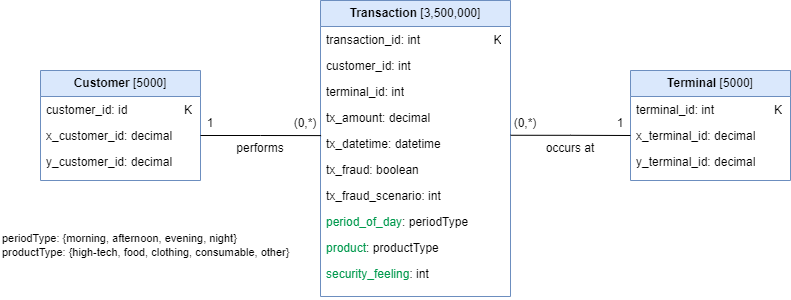
\includegraphics{images/conceptual-model.png}
\caption{conceptual-model}
\end{figure}

    \hypertarget{assumptions}{%
\subsection{Assumptions}\label{assumptions}}

    There are several considerations taken into account regarding the design
of the conceptual model, which we organize as below:

\begin{itemize}
\tightlist
\item
  \textbf{Customer Profiles:} There are several properties proposed by
  the simulator that were only required for the dataset generation and
  will no longer be needed in the remainder of the analysis, hence we
  can exclude them.

  \begin{itemize}
  \tightlist
  \item
    The \texttt{available\_terminals} property of a customer only
    demonstrates the terminals located in the specified radius of the
    customer (in a 100 by 100 grid) that are accessible by the customer,
    which is used to randomly make connections to a subset of these
    available terminals. However, this property does not necessarily
    reflect the \emph{actual} terminal nodes to which the customer is
    connected and provides no information. In addition, since this
    property holds a list, it might explode when the number of terminals
    in the radius increases and takes a lot of storage, so we can
    discard it from the domain. With the same intuition,
    \texttt{nb\_terminals} should also be removed, since it only reports
    the number of available terminals.
  \item
    The \texttt{mean\_amount} and \texttt{std\_amount} properties of the
    customer are only used to generate the transaction amounts
    respecting a uniform distribution, and are not further used in the
    analysis, hence they can be removed.
  \item
    The average number of transactions per day for the customer denoted
    as \texttt{mean\_nb\_tx\_per\_day} is used in the generation of the
    transactions, and is no longer needed.
  \end{itemize}
\item
  \textbf{Terminal Profiles:} Terminal profiles contain only
  geographical details aside from the \texttt{terminal\_id}. Although
  the coordinates are not used during the analysis, we attempt to keep
  this information.
\item
  \textbf{Transactions:} All the properties in the transactions data are
  later used to either provide statistics on the dataset or perform
  queries. Therefore, we keep all this information intact. However, the
  properties \texttt{tx\_time\_seconds} and \texttt{tx\_time\_days} are
  not useful at all in the proposed workload, and we will discard them.
  We should note that according to the generated transactions, we have a
  \texttt{transaction\_id} field that can uniquely identify a
  transaction, without requiring the \texttt{customer\_id} and
  \texttt{terminal\_id} to be used as the primary key.
\end{itemize}

    \hypertarget{constraints}{%
\subsection{Constraints}\label{constraints}}

    \begin{itemize}
\tightlist
\item
  The overall objective of this study is to detect fraudulent
  transactions. The attributes \texttt{tx\_fraud} and
  \texttt{tx\_fraud\_scenario} are introduced and initialized upon
  dataset creation, and do not necessarily reflect whether a transaction
  is fraudulent or genuine. These properties should be updated later
  with proper information by the fraud detection techniques.
\item
  As mentioned in the assumptions, the attributes
  \texttt{available\_terminals}, \texttt{nb\_terminals},
  \texttt{mean\_amount}, \texttt{std\_amount}, and
  \texttt{mean\_nb\_tx\_per\_day} were only utilized to generate the
  initial datasets, so we decided to exclude them. If we wish to keep
  these attributes, they have to be constantly updated on each
  transaction made by the customer.
\item
  Data validation techniques should be enforced to ensure that the
  inserted data respects the required data types. As an example, since
  the coordinates grid dimensions are \(100 \times 100\), the
  \texttt{x\_customer\_id}, \texttt{y\_customer\_id},
  \texttt{x\_terminal\_id}, and \texttt{y\_terminal\_id} attributes
  should be constrained within (0,100). Also, \texttt{period\_of\_day}
  and \texttt{product} should be only selected from the specified set of
  predefined values, and the \texttt{security\_feeling} can be impressed
  as an integer number within (1,5).
\end{itemize}

    \hypertarget{logical-model}{%
\section{Logical Model}\label{logical-model}}

    For the proposed domain and the requested workload, it is the best
option to store and query these data in a graph database. Several
factors are involved in taking this decision:

\begin{itemize}
\tightlist
\item
  \textbf{Simplicity:} Using a graph database (e.g.~Neo4j), it is
  extremely convenient to store and navigate the transaction data. We
  can represent the customers and terminals as nodes of the graph, and
  transactions can be treated as the edges. Despite the simplicity, this
  design is powerful enough to cover all the requested queries in the
  workload without requiring complex queries.
\item
  \textbf{Performance:} Since the data is organized as a graph, it would
  have the best performance when trying to identify a path along the
  graph, hence the highest performance is achieved.
\item
  \textbf{Powerful:} The workload requires us to store different kinds
  of relationships, and to be able to infer based on them. Since these
  relationships are stored simply as the edges of the graph, there is no
  trouble in the management of these relationships.
\end{itemize}

In order to shape the graph with nodes and edges, we need to make
decisions on the entities of our conceptual model. The \texttt{Customer}
and \texttt{Terminal} entities will be demonstrated as nodes in the
graph, having labels of \texttt{:Customer} and \texttt{:Terminal}
respectively. However, for \texttt{Transaction} entities we have two
possible design choices:

\begin{enumerate}
\def\labelenumi{\arabic{enumi}.}
\tightlist
\item
  Shaping the graph as
  \texttt{(:Customer)-{[}:MAKES{]}-\textgreater{}(:Transaction)-{[}:AT{]}-\textgreater{}(:Terminal)},
  we can define the transactions as separate \emph{nodes}. However, this
  representation of the data may be redundant, simply because we have no
  direct use of the relationships \texttt{:MAKES} and \texttt{:AT} in
  the workload, and also there are no additional properties to be
  assigned to these relationships.
\item
  We can shape the graph as
  \texttt{(:Customer)-{[}:TRANSACTION{]}-\textgreater{}(:Terminal)},
  where we keep the transactions simply as a relationship between
  customers and terminals. Using property graph databases such as Neo4j,
  it is possible to define properties for the transactions on the edges
  of the graph as well.
\end{enumerate}

As discussed, we will proceed with the second approach due to its
simplicity and efficiency. Without any further hesitations, we will now
present the logical model designed for a graph database, which we will
later implement in Neo4j. Keep in mind, that the green-pained edges and
attributes are the ones that are introduced later to be stored in the
graph.

\begin{figure}
\centering
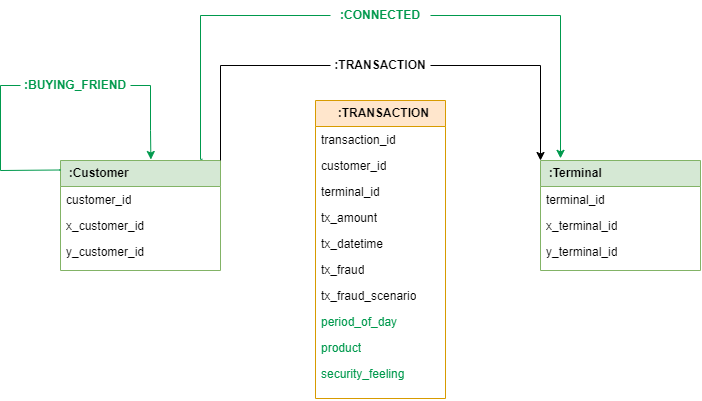
\includegraphics{images/logical-model.png}
\caption{logical-model}
\end{figure}


    \hypertarget{transaction-graph-generation}{%
\section{Transaction Graph
Generation}\label{transaction-graph-generation}}

    Using the building blocks of the transaction data simulator, we will
proceed with inserting the data into our Neo4j databases. In this
section, we will first generate the transaction graph, and then discuss
the execution times for inserting the data into each graph.

    \hypertarget{generation-of-the-transaction-graphs}{%
\subsection{Generation of the Transaction
Graphs}\label{generation-of-the-transaction-graphs}}

    The objective of this project is to first create 3 different databases
of sizes 50Mb, 100Mb, and 200Mb, respectively. The following steps are
taken sequentially to achieve this:

\begin{itemize}
\tightlist
\item
  In the first step, we have to create a database in the Neo4j Desktop
  application, let's name it \texttt{TransactionGraph}. We set
  \texttt{user\ =\ "neo4j",\ password="12345678"} as the required
  authentications.
\item
  We run the \texttt{TransactionGraph} on the default bold URI
  \texttt{bolt://localhost:7687}.
\item
  We attempt to create three different databases, namely \texttt{TG50},
  \texttt{TG100}, and \texttt{TG200}, respectively. The naming
  convention denotes the desired size of data to be stored in each of
  the databases. An additional \texttt{TGtest} database would be also
  created for test purposes.
\item
  Using the Python cells below, we will insert the generated dataset for
  each of the databases separately, and automatically insert it into the
  database. We will store the execution times to report later as well.
  It is important to mention that to achieve the mentioned goals on a
  local server containing the Neo4j Desctop application, we have to run
  the script locally (not on platforms like Google Colab).
\end{itemize}

    \begin{tcolorbox}[breakable, size=fbox, boxrule=1pt, pad at break*=1mm,colback=cellbackground, colframe=cellborder]
\prompt{In}{incolor}{13}{\boxspacing}
\begin{Verbatim}[commandchars=\\\{\}]
\PY{k}{class} \PY{n+nc}{Database}\PY{p}{:}
    \PY{k}{def} \PY{n+nf+fm}{\PYZus{}\PYZus{}init\PYZus{}\PYZus{}}\PY{p}{(}\PY{n+nb+bp}{self}\PY{p}{)}\PY{p}{:}
        \PY{n+nb+bp}{self}\PY{o}{.}\PY{n}{batch\PYZus{}size} \PY{o}{=} \PY{l+m+mi}{200}
        \PY{n+nb+bp}{self}\PY{o}{.}\PY{n}{auth} \PY{o}{=} \PY{p}{\PYZob{}}
            \PY{l+s+s2}{\PYZdq{}}\PY{l+s+s2}{uri}\PY{l+s+s2}{\PYZdq{}}\PY{p}{:} \PY{l+s+s2}{\PYZdq{}}\PY{l+s+s2}{bolt://localhost:7687}\PY{l+s+s2}{\PYZdq{}}\PY{p}{,}
            \PY{l+s+s2}{\PYZdq{}}\PY{l+s+s2}{user}\PY{l+s+s2}{\PYZdq{}}\PY{p}{:} \PY{l+s+s2}{\PYZdq{}}\PY{l+s+s2}{neo4j}\PY{l+s+s2}{\PYZdq{}}\PY{p}{,}
            \PY{l+s+s2}{\PYZdq{}}\PY{l+s+s2}{password}\PY{l+s+s2}{\PYZdq{}}\PY{p}{:} \PY{l+s+s2}{\PYZdq{}}\PY{l+s+s2}{12345678}\PY{l+s+s2}{\PYZdq{}}
        \PY{p}{\PYZcb{}}
        \PY{n+nb+bp}{self}\PY{o}{.}\PY{n}{driver} \PY{o}{=} \PY{n}{GraphDatabase}\PY{o}{.}\PY{n}{driver}\PY{p}{(}
            \PY{n+nb+bp}{self}\PY{o}{.}\PY{n}{auth}\PY{p}{[}\PY{l+s+s1}{\PYZsq{}}\PY{l+s+s1}{uri}\PY{l+s+s1}{\PYZsq{}}\PY{p}{]}\PY{p}{,}
            \PY{n}{auth}\PY{o}{=}\PY{p}{(}\PY{n+nb+bp}{self}\PY{o}{.}\PY{n}{auth}\PY{p}{[}\PY{l+s+s1}{\PYZsq{}}\PY{l+s+s1}{user}\PY{l+s+s1}{\PYZsq{}}\PY{p}{]}\PY{p}{,} \PY{n+nb+bp}{self}\PY{o}{.}\PY{n}{auth}\PY{p}{[}\PY{l+s+s1}{\PYZsq{}}\PY{l+s+s1}{password}\PY{l+s+s1}{\PYZsq{}}\PY{p}{]}\PY{p}{)}
        \PY{p}{)}
        \PY{n+nb+bp}{self}\PY{o}{.}\PY{n}{set\PYZus{}create\PYZus{}queries}\PY{p}{(}\PY{p}{)}
        \PY{n+nb+bp}{self}\PY{o}{.}\PY{n}{create\PYZus{}execution\PYZus{}times} \PY{o}{=} \PY{n+nb}{dict}\PY{p}{(}\PY{p}{)}
        \PY{n+nb+bp}{self}\PY{o}{.}\PY{n}{read\PYZus{}execution\PYZus{}times} \PY{o}{=} \PY{n+nb}{dict}\PY{p}{(}\PY{p}{)}

    \PY{k}{def} \PY{n+nf}{set\PYZus{}create\PYZus{}queries}\PY{p}{(}\PY{n+nb+bp}{self}\PY{p}{)}\PY{p}{:}
\PY{+w}{        }\PY{l+s+sd}{\PYZsq{}\PYZsq{}\PYZsq{}}
\PY{l+s+sd}{        For ease of use, we store all the \PYZdq{}create\PYZdq{} queries for adding new nodes/edges}
\PY{l+s+sd}{        in the class, which are easily accessible when needed}
\PY{l+s+sd}{        \PYZsq{}\PYZsq{}\PYZsq{}}
        
        \PY{n+nb+bp}{self}\PY{o}{.}\PY{n}{create\PYZus{}customer\PYZus{}query} \PY{o}{=} \PY{l+s+s2}{\PYZdq{}\PYZdq{}\PYZdq{}}
\PY{l+s+s2}{            UNWIND \PYZdl{}data AS customer}
\PY{l+s+s2}{            CREATE (c:Customer }\PY{l+s+s2}{\PYZob{}}
\PY{l+s+s2}{                customer\PYZus{}id: customer[}\PY{l+s+s2}{\PYZsq{}}\PY{l+s+s2}{CUSTOMER\PYZus{}ID}\PY{l+s+s2}{\PYZsq{}}\PY{l+s+s2}{],}
\PY{l+s+s2}{                x\PYZus{}customer\PYZus{}id: customer[}\PY{l+s+s2}{\PYZsq{}}\PY{l+s+s2}{x\PYZus{}customer\PYZus{}id}\PY{l+s+s2}{\PYZsq{}}\PY{l+s+s2}{],}
\PY{l+s+s2}{                y\PYZus{}customer\PYZus{}id: customer[}\PY{l+s+s2}{\PYZsq{}}\PY{l+s+s2}{y\PYZus{}customer\PYZus{}id}\PY{l+s+s2}{\PYZsq{}}\PY{l+s+s2}{]}
\PY{l+s+s2}{            \PYZcb{})}
\PY{l+s+s2}{        }\PY{l+s+s2}{\PYZdq{}\PYZdq{}\PYZdq{}}
        
        \PY{n+nb+bp}{self}\PY{o}{.}\PY{n}{create\PYZus{}terminal\PYZus{}query} \PY{o}{=} \PY{l+s+s2}{\PYZdq{}\PYZdq{}\PYZdq{}}
\PY{l+s+s2}{            UNWIND \PYZdl{}data AS terminal}
\PY{l+s+s2}{            CREATE (t:Terminal }\PY{l+s+s2}{\PYZob{}}
\PY{l+s+s2}{                terminal\PYZus{}id: terminal[}\PY{l+s+s2}{\PYZsq{}}\PY{l+s+s2}{TERMINAL\PYZus{}ID}\PY{l+s+s2}{\PYZsq{}}\PY{l+s+s2}{],}
\PY{l+s+s2}{                x\PYZus{}terminal\PYZus{}id: terminal[}\PY{l+s+s2}{\PYZsq{}}\PY{l+s+s2}{x\PYZus{}terminal\PYZus{}id}\PY{l+s+s2}{\PYZsq{}}\PY{l+s+s2}{],}
\PY{l+s+s2}{                y\PYZus{}terminal\PYZus{}id: terminal[}\PY{l+s+s2}{\PYZsq{}}\PY{l+s+s2}{y\PYZus{}terminal\PYZus{}id}\PY{l+s+s2}{\PYZsq{}}\PY{l+s+s2}{]}
\PY{l+s+s2}{            \PYZcb{})}
\PY{l+s+s2}{        }\PY{l+s+s2}{\PYZdq{}\PYZdq{}\PYZdq{}}
        
        \PY{n+nb+bp}{self}\PY{o}{.}\PY{n}{create\PYZus{}transaction\PYZus{}query} \PY{o}{=} \PY{l+s+s2}{\PYZdq{}\PYZdq{}\PYZdq{}}
\PY{l+s+s2}{            UNWIND \PYZdl{}data AS transaction}
\PY{l+s+s2}{            MATCH (c:Customer }\PY{l+s+s2}{\PYZob{}}\PY{l+s+s2}{customer\PYZus{}id: transaction[}\PY{l+s+s2}{\PYZsq{}}\PY{l+s+s2}{CUSTOMER\PYZus{}ID}\PY{l+s+s2}{\PYZsq{}}\PY{l+s+s2}{]\PYZcb{})}
\PY{l+s+s2}{            MATCH (t:Terminal }\PY{l+s+s2}{\PYZob{}}\PY{l+s+s2}{terminal\PYZus{}id: transaction[}\PY{l+s+s2}{\PYZsq{}}\PY{l+s+s2}{TERMINAL\PYZus{}ID}\PY{l+s+s2}{\PYZsq{}}\PY{l+s+s2}{]\PYZcb{})}
\PY{l+s+s2}{            CREATE (c)\PYZhy{}[:TRANSACTION }\PY{l+s+s2}{\PYZob{}}
\PY{l+s+s2}{                transaction\PYZus{}id: transaction[}\PY{l+s+s2}{\PYZsq{}}\PY{l+s+s2}{TRANSACTION\PYZus{}ID}\PY{l+s+s2}{\PYZsq{}}\PY{l+s+s2}{],}
\PY{l+s+s2}{                customer\PYZus{}id: transaction[}\PY{l+s+s2}{\PYZsq{}}\PY{l+s+s2}{CUSTOMER\PYZus{}ID}\PY{l+s+s2}{\PYZsq{}}\PY{l+s+s2}{],}
\PY{l+s+s2}{                terminal\PYZus{}id: transaction[}\PY{l+s+s2}{\PYZsq{}}\PY{l+s+s2}{TERMINAL\PYZus{}ID}\PY{l+s+s2}{\PYZsq{}}\PY{l+s+s2}{],}
\PY{l+s+s2}{                tx\PYZus{}amount: transaction[}\PY{l+s+s2}{\PYZsq{}}\PY{l+s+s2}{TX\PYZus{}AMOUNT}\PY{l+s+s2}{\PYZsq{}}\PY{l+s+s2}{],}
\PY{l+s+s2}{                tx\PYZus{}datetime: transaction[}\PY{l+s+s2}{\PYZsq{}}\PY{l+s+s2}{TX\PYZus{}DATETIME}\PY{l+s+s2}{\PYZsq{}}\PY{l+s+s2}{],}
\PY{l+s+s2}{                tx\PYZus{}fraud: transaction[}\PY{l+s+s2}{\PYZsq{}}\PY{l+s+s2}{TX\PYZus{}FRAUD}\PY{l+s+s2}{\PYZsq{}}\PY{l+s+s2}{],}
\PY{l+s+s2}{                tx\PYZus{}fraud\PYZus{}scenario: transaction[}\PY{l+s+s2}{\PYZsq{}}\PY{l+s+s2}{TX\PYZus{}FRAUD\PYZus{}SCENARIO}\PY{l+s+s2}{\PYZsq{}}\PY{l+s+s2}{]}
\PY{l+s+s2}{            \PYZcb{}]\PYZhy{}\PYZgt{}(t)}
\PY{l+s+s2}{        }\PY{l+s+s2}{\PYZdq{}\PYZdq{}\PYZdq{}}
        
    \PY{k}{def} \PY{n+nf}{print\PYZus{}data\PYZus{}size}\PY{p}{(}\PY{n+nb+bp}{self}\PY{p}{,} \PY{n}{customer\PYZus{}profiles\PYZus{}table}\PY{p}{,} \PY{n}{terminal\PYZus{}profiles\PYZus{}table}\PY{p}{,} \PY{n}{transactions\PYZus{}df}\PY{p}{)}\PY{p}{:}
\PY{+w}{        }\PY{l+s+sd}{\PYZsq{}\PYZsq{}\PYZsq{}}
\PY{l+s+sd}{        It is difficult to estimate the exact size of the database before storing it,}
\PY{l+s+sd}{        hence we use `memory\PYZus{}usage` of DataFrames to estimate an approximate value}
\PY{l+s+sd}{        \PYZsq{}\PYZsq{}\PYZsq{}}
        \PY{c+c1}{\PYZsh{} Computing the total storage size of data}
        \PY{n}{dataframes} \PY{o}{=} \PY{p}{[}\PY{n}{customer\PYZus{}profiles\PYZus{}table}\PY{p}{,} \PY{n}{terminal\PYZus{}profiles\PYZus{}table}\PY{p}{,} \PY{n}{transactions\PYZus{}df}\PY{p}{]}
        \PY{n}{total\PYZus{}memory\PYZus{}mb} \PY{o}{=} \PY{n+nb}{sum}\PY{p}{(}\PY{n}{df}\PY{o}{.}\PY{n}{memory\PYZus{}usage}\PY{p}{(}\PY{n}{deep}\PY{o}{=}\PY{k+kc}{True}\PY{p}{)}\PY{o}{.}\PY{n}{sum}\PY{p}{(}\PY{p}{)} \PY{k}{for} \PY{n}{df} \PY{o+ow}{in} \PY{n}{dataframes}\PY{p}{)} \PY{o}{/} \PY{p}{(}\PY{l+m+mi}{1024} \PY{o}{*} \PY{l+m+mi}{1024}\PY{p}{)}
        \PY{n+nb}{print}\PY{p}{(}\PY{l+s+sa}{f}\PY{l+s+s2}{\PYZdq{}}\PY{l+s+s2}{Total storage size of data: }\PY{l+s+si}{\PYZob{}}\PY{n}{total\PYZus{}memory\PYZus{}mb}\PY{l+s+si}{:}\PY{l+s+s2}{.2f}\PY{l+s+si}{\PYZcb{}}\PY{l+s+s2}{ MB}\PY{l+s+s2}{\PYZdq{}}\PY{p}{)}

    \PY{k}{def} \PY{n+nf}{transform\PYZus{}data}\PY{p}{(}\PY{n+nb+bp}{self}\PY{p}{,} \PY{n}{customer\PYZus{}profiles\PYZus{}table}\PY{p}{,} \PY{n}{terminal\PYZus{}profiles\PYZus{}table}\PY{p}{,} \PY{n}{transactions\PYZus{}df}\PY{p}{)}\PY{p}{:}
\PY{+w}{        }\PY{l+s+sd}{\PYZsq{}\PYZsq{}\PYZsq{}}
\PY{l+s+sd}{        In order to insert the data into Neo4j database using Python connector, we need}
\PY{l+s+sd}{        to transform the DataFrame objects into lists of JSONs. Next, to prevent the }
\PY{l+s+sd}{        session breaks and enhance the data insertion into the graph, we transform the}
\PY{l+s+sd}{        obtained list into batches of JSONs}
\PY{l+s+sd}{        \PYZsq{}\PYZsq{}\PYZsq{}}
        
        \PY{c+c1}{\PYZsh{} Convert DataFrames to lists of dictionaries}
        \PY{n}{customers\PYZus{}data} \PY{o}{=} \PY{n}{customer\PYZus{}profiles\PYZus{}table}\PY{o}{.}\PY{n}{to\PYZus{}dict}\PY{p}{(}\PY{n}{orient}\PY{o}{=}\PY{l+s+s1}{\PYZsq{}}\PY{l+s+s1}{records}\PY{l+s+s1}{\PYZsq{}}\PY{p}{)}
        \PY{n}{terminals\PYZus{}data} \PY{o}{=} \PY{n}{terminal\PYZus{}profiles\PYZus{}table}\PY{o}{.}\PY{n}{to\PYZus{}dict}\PY{p}{(}\PY{n}{orient}\PY{o}{=}\PY{l+s+s1}{\PYZsq{}}\PY{l+s+s1}{records}\PY{l+s+s1}{\PYZsq{}}\PY{p}{)}
        \PY{n}{transactions\PYZus{}data} \PY{o}{=} \PY{n}{transactions\PYZus{}df}\PY{o}{.}\PY{n}{to\PYZus{}dict}\PY{p}{(}\PY{n}{orient}\PY{o}{=}\PY{l+s+s1}{\PYZsq{}}\PY{l+s+s1}{records}\PY{l+s+s1}{\PYZsq{}}\PY{p}{)}
    
        \PY{c+c1}{\PYZsh{} Create batches of data for efficient insertion}
        \PY{n}{batch\PYZus{}creator} \PY{o}{=} \PY{k}{lambda} \PY{n}{data}\PY{p}{:} \PYZbs{}
            \PY{p}{[}\PY{n}{data}\PY{p}{[}\PY{n}{i}\PY{p}{:}\PY{n}{i} \PY{o}{+} \PY{n+nb+bp}{self}\PY{o}{.}\PY{n}{batch\PYZus{}size}\PY{p}{]} \PY{k}{for} \PY{n}{i} \PY{o+ow}{in} \PY{n+nb}{range}\PY{p}{(}\PY{l+m+mi}{0}\PY{p}{,} \PY{n+nb}{len}\PY{p}{(}\PY{n}{data}\PY{p}{)}\PY{p}{,} \PY{n+nb+bp}{self}\PY{o}{.}\PY{n}{batch\PYZus{}size}\PY{p}{)}\PY{p}{]}
        \PY{n}{customers\PYZus{}batch} \PY{o}{=} \PY{n}{batch\PYZus{}creator}\PY{p}{(}\PY{n}{customers\PYZus{}data}\PY{p}{)}
        \PY{n}{terminals\PYZus{}batch} \PY{o}{=} \PY{n}{batch\PYZus{}creator}\PY{p}{(}\PY{n}{terminals\PYZus{}data}\PY{p}{)}
        \PY{n}{transactions\PYZus{}batch} \PY{o}{=} \PY{n}{batch\PYZus{}creator}\PY{p}{(}\PY{n}{transactions\PYZus{}data}\PY{p}{)}
        \PY{k}{return} \PY{n}{customers\PYZus{}batch}\PY{p}{,} \PY{n}{terminals\PYZus{}batch}\PY{p}{,} \PY{n}{transactions\PYZus{}batch}

    \PY{k}{def} \PY{n+nf}{batch\PYZus{}insert}\PY{p}{(}\PY{n+nb+bp}{self}\PY{p}{,} \PY{n}{session}\PY{p}{,} \PY{n}{query}\PY{p}{,} \PY{n}{data\PYZus{}batch}\PY{p}{,} \PY{n}{data\PYZus{}type}\PY{p}{)}\PY{p}{:}
\PY{+w}{        }\PY{l+s+sd}{\PYZsq{}\PYZsq{}\PYZsq{}}
\PY{l+s+sd}{        This function runs a single \PYZdq{}create\PYZdq{} query on Neo4j and displays a progress bar}
\PY{l+s+sd}{        showing the amount of time taken to insert the data}
\PY{l+s+sd}{        \PYZsq{}\PYZsq{}\PYZsq{}}
        \PY{n}{progressBar} \PY{o}{=} \PY{n}{tqdm}\PY{p}{(}\PY{n}{data\PYZus{}batch}\PY{p}{)}
        \PY{k}{for} \PY{n}{i}\PY{p}{,} \PY{n}{batch} \PY{o+ow}{in} \PY{n+nb}{enumerate}\PY{p}{(}\PY{n}{progressBar}\PY{p}{)}\PY{p}{:}
            \PY{n}{progressBar}\PY{o}{.}\PY{n}{set\PYZus{}description}\PY{p}{(}\PY{l+s+sa}{f}\PY{l+s+s1}{\PYZsq{}}\PY{l+s+s1}{Inserting }\PY{l+s+si}{\PYZob{}}\PY{n}{data\PYZus{}type}\PY{l+s+si}{\PYZcb{}}\PY{l+s+s1}{ data (batches of size }\PY{l+s+si}{\PYZob{}}\PY{n+nb+bp}{self}\PY{o}{.}\PY{n}{batch\PYZus{}size}\PY{l+s+si}{\PYZcb{}}\PY{l+s+s1}{)}\PY{l+s+s1}{\PYZsq{}}\PY{p}{)}
            \PY{n}{session}\PY{o}{.}\PY{n}{run}\PY{p}{(}\PY{n}{query}\PY{p}{,} \PY{n}{data}\PY{o}{=}\PY{n}{batch}\PY{p}{)}

    \PY{k}{def} \PY{n+nf}{batch\PYZus{}insert\PYZus{}into\PYZus{}db}\PY{p}{(}\PY{n+nb+bp}{self}\PY{p}{,} \PY{n}{database}\PY{p}{,} \PY{n}{customers\PYZus{}batch}\PY{p}{,} \PY{n}{terminals\PYZus{}batch}\PY{p}{,} \PY{n}{transactions\PYZus{}batch}\PY{p}{)}\PY{p}{:}
\PY{+w}{        }\PY{l+s+sd}{\PYZsq{}\PYZsq{}\PYZsq{}}
\PY{l+s+sd}{        This function utilizes the `batch\PYZus{}insert` function to run the create queries}
\PY{l+s+sd}{        on the suggested database within Neo4j, and insert the data as a graph}
\PY{l+s+sd}{        \PYZsq{}\PYZsq{}\PYZsq{}}
        \PY{k}{with} \PY{n+nb+bp}{self}\PY{o}{.}\PY{n}{driver}\PY{o}{.}\PY{n}{session}\PY{p}{(}\PY{n}{database}\PY{o}{=}\PY{n}{database}\PY{p}{)} \PY{k}{as} \PY{n}{session}\PY{p}{:}
            \PY{n}{t\PYZus{}start} \PY{o}{=} \PY{n}{time}\PY{o}{.}\PY{n}{time}\PY{p}{(}\PY{p}{)}
            \PY{n+nb+bp}{self}\PY{o}{.}\PY{n}{batch\PYZus{}insert}\PY{p}{(}\PY{n}{session}\PY{p}{,} \PY{n+nb+bp}{self}\PY{o}{.}\PY{n}{create\PYZus{}customer\PYZus{}query}\PY{p}{,} \PY{n}{customers\PYZus{}batch}\PY{p}{,} \PY{n}{data\PYZus{}type}\PY{o}{=}\PY{l+s+s1}{\PYZsq{}}\PY{l+s+s1}{customers}\PY{l+s+s1}{\PYZsq{}}\PY{p}{)}
            \PY{n+nb+bp}{self}\PY{o}{.}\PY{n}{batch\PYZus{}insert}\PY{p}{(}\PY{n}{session}\PY{p}{,} \PY{n+nb+bp}{self}\PY{o}{.}\PY{n}{create\PYZus{}terminal\PYZus{}query}\PY{p}{,} \PY{n}{terminals\PYZus{}batch}\PY{p}{,} \PY{n}{data\PYZus{}type}\PY{o}{=}\PY{l+s+s1}{\PYZsq{}}\PY{l+s+s1}{terminals}\PY{l+s+s1}{\PYZsq{}}\PY{p}{)}
            \PY{n+nb+bp}{self}\PY{o}{.}\PY{n}{batch\PYZus{}insert}\PY{p}{(}\PY{n}{session}\PY{p}{,} \PY{n+nb+bp}{self}\PY{o}{.}\PY{n}{create\PYZus{}transaction\PYZus{}query}\PY{p}{,} \PY{n}{transactions\PYZus{}batch}\PY{p}{,} \PY{n}{data\PYZus{}type}\PY{o}{=}\PY{l+s+s1}{\PYZsq{}}\PY{l+s+s1}{transactions}\PY{l+s+s1}{\PYZsq{}}\PY{p}{)}
            \PY{n}{t\PYZus{}total} \PY{o}{=} \PY{n+nb}{round}\PY{p}{(}\PY{n}{time}\PY{o}{.}\PY{n}{time}\PY{p}{(}\PY{p}{)} \PY{o}{\PYZhy{}} \PY{n}{t\PYZus{}start}\PY{p}{,} \PY{l+m+mi}{3}\PY{p}{)}
            \PY{n+nb+bp}{self}\PY{o}{.}\PY{n}{create\PYZus{}execution\PYZus{}times}\PY{p}{[}\PY{n}{database}\PY{p}{]} \PY{o}{=} \PY{n}{t\PYZus{}total}

    \PY{k}{def} \PY{n+nf}{get\PYZus{}stats}\PY{p}{(}\PY{n+nb+bp}{self}\PY{p}{,} \PY{n}{transactions\PYZus{}df}\PY{p}{)}\PY{p}{:}
        \PY{c+c1}{\PYZsh{}Number of transactions per day}
        \PY{n}{nb\PYZus{}tx\PYZus{}per\PYZus{}day}\PY{o}{=}\PY{n}{transactions\PYZus{}df}\PY{o}{.}\PY{n}{groupby}\PY{p}{(}\PY{p}{[}\PY{l+s+s1}{\PYZsq{}}\PY{l+s+s1}{TX\PYZus{}TIME\PYZus{}DAYS}\PY{l+s+s1}{\PYZsq{}}\PY{p}{]}\PY{p}{)}\PY{p}{[}\PY{l+s+s1}{\PYZsq{}}\PY{l+s+s1}{CUSTOMER\PYZus{}ID}\PY{l+s+s1}{\PYZsq{}}\PY{p}{]}\PY{o}{.}\PY{n}{count}\PY{p}{(}\PY{p}{)}
        \PY{c+c1}{\PYZsh{}Number of fraudulent transactions per day}
        \PY{n}{nb\PYZus{}fraud\PYZus{}per\PYZus{}day}\PY{o}{=}\PY{n}{transactions\PYZus{}df}\PY{o}{.}\PY{n}{groupby}\PY{p}{(}\PY{p}{[}\PY{l+s+s1}{\PYZsq{}}\PY{l+s+s1}{TX\PYZus{}TIME\PYZus{}DAYS}\PY{l+s+s1}{\PYZsq{}}\PY{p}{]}\PY{p}{)}\PY{p}{[}\PY{l+s+s1}{\PYZsq{}}\PY{l+s+s1}{TX\PYZus{}FRAUD}\PY{l+s+s1}{\PYZsq{}}\PY{p}{]}\PY{o}{.}\PY{n}{sum}\PY{p}{(}\PY{p}{)}
        \PY{c+c1}{\PYZsh{}Number of fraudulent cards per day}
        \PY{n}{nb\PYZus{}fraudcard\PYZus{}per\PYZus{}day}\PY{o}{=}\PY{n}{transactions\PYZus{}df}\PY{p}{[}\PY{n}{transactions\PYZus{}df}\PY{p}{[}\PY{l+s+s1}{\PYZsq{}}\PY{l+s+s1}{TX\PYZus{}FRAUD}\PY{l+s+s1}{\PYZsq{}}\PY{p}{]}\PY{o}{\PYZgt{}}\PY{l+m+mi}{0}\PY{p}{]}\PY{o}{.}\PY{n}{groupby}\PY{p}{(}\PY{p}{[}\PY{l+s+s1}{\PYZsq{}}\PY{l+s+s1}{TX\PYZus{}TIME\PYZus{}DAYS}\PY{l+s+s1}{\PYZsq{}}\PY{p}{]}\PY{p}{)}\PY{o}{.}\PY{n}{CUSTOMER\PYZus{}ID}\PY{o}{.}\PY{n}{nunique}\PY{p}{(}\PY{p}{)}
        \PY{k}{return} \PY{p}{(}\PY{n}{nb\PYZus{}tx\PYZus{}per\PYZus{}day}\PY{p}{,}\PY{n}{nb\PYZus{}fraud\PYZus{}per\PYZus{}day}\PY{p}{,}\PY{n}{nb\PYZus{}fraudcard\PYZus{}per\PYZus{}day}\PY{p}{)}
    
    \PY{k}{def} \PY{n+nf}{plot\PYZus{}stats}\PY{p}{(}\PY{n+nb+bp}{self}\PY{p}{,} \PY{n}{transactions\PYZus{}df}\PY{p}{,} \PY{n}{database}\PY{p}{)}\PY{p}{:}
        \PY{c+c1}{\PYZsh{} PLOTTING THE DISTRIBUTIONS \PYZhy{}\PYZhy{}\PYZhy{}\PYZhy{}\PYZhy{}\PYZhy{}\PYZhy{}\PYZhy{}\PYZhy{}\PYZhy{}\PYZhy{}\PYZhy{}\PYZhy{}\PYZhy{}\PYZhy{}\PYZhy{}\PYZhy{}\PYZhy{}\PYZhy{}\PYZhy{}\PYZhy{}\PYZhy{}\PYZhy{}\PYZhy{}\PYZhy{}\PYZhy{}\PYZhy{}\PYZhy{}\PYZhy{}\PYZhy{}\PYZhy{}\PYZhy{}\PYZhy{}\PYZhy{}\PYZhy{}\PYZhy{}\PYZhy{}\PYZhy{}\PYZhy{}\PYZhy{}\PYZhy{}\PYZhy{}\PYZhy{}\PYZhy{}\PYZhy{}\PYZhy{}\PYZhy{}\PYZhy{}\PYZhy{}\PYZhy{}\PYZhy{}\PYZhy{}\PYZhy{}\PYZhy{}\PYZhy{}\PYZhy{}\PYZhy{}}
        \PY{n}{distribution\PYZus{}amount\PYZus{}times\PYZus{}fig}\PY{p}{,} \PY{n}{ax} \PY{o}{=} \PY{n}{plt}\PY{o}{.}\PY{n}{subplots}\PY{p}{(}\PY{l+m+mi}{1}\PY{p}{,} \PY{l+m+mi}{2}\PY{p}{,} \PY{n}{figsize}\PY{o}{=}\PY{p}{(}\PY{l+m+mi}{18}\PY{p}{,}\PY{l+m+mi}{4}\PY{p}{)}\PY{p}{)}
        \PY{n}{n\PYZus{}samples} \PY{o}{=} \PY{n+nb}{min}\PY{p}{(}\PY{n+nb}{len}\PY{p}{(}\PY{n}{transactions\PYZus{}df}\PY{p}{)}\PY{p}{,} \PY{l+m+mi}{10000}\PY{p}{)}
        \PY{n}{amount\PYZus{}val} \PY{o}{=} \PY{n}{transactions\PYZus{}df}\PY{p}{[}\PY{n}{transactions\PYZus{}df}\PY{o}{.}\PY{n}{TX\PYZus{}TIME\PYZus{}DAYS}\PY{o}{\PYZlt{}}\PY{l+m+mi}{10}\PY{p}{]}\PY{p}{[}\PY{l+s+s1}{\PYZsq{}}\PY{l+s+s1}{TX\PYZus{}AMOUNT}\PY{l+s+s1}{\PYZsq{}}\PY{p}{]}\PY{o}{.}\PY{n}{sample}\PY{p}{(}\PY{n}{n}\PY{o}{=}\PY{n}{n\PYZus{}samples}\PY{p}{,} \PY{n}{replace}\PY{o}{=}\PY{k+kc}{True}\PY{p}{)}\PY{o}{.}\PY{n}{values}
        \PY{n}{time\PYZus{}val} \PY{o}{=} \PY{n}{transactions\PYZus{}df}\PY{p}{[}\PY{n}{transactions\PYZus{}df}\PY{o}{.}\PY{n}{TX\PYZus{}TIME\PYZus{}DAYS}\PY{o}{\PYZlt{}}\PY{l+m+mi}{10}\PY{p}{]}\PY{p}{[}\PY{l+s+s1}{\PYZsq{}}\PY{l+s+s1}{TX\PYZus{}TIME\PYZus{}SECONDS}\PY{l+s+s1}{\PYZsq{}}\PY{p}{]}\PY{o}{.}\PY{n}{sample}\PY{p}{(}\PY{n}{n}\PY{o}{=}\PY{n}{n\PYZus{}samples}\PY{p}{,} \PY{n}{replace}\PY{o}{=}\PY{k+kc}{True}\PY{p}{)}\PY{o}{.}\PY{n}{values}
        
        \PY{n}{sns}\PY{o}{.}\PY{n}{distplot}\PY{p}{(}\PY{n}{amount\PYZus{}val}\PY{p}{,} \PY{n}{ax}\PY{o}{=}\PY{n}{ax}\PY{p}{[}\PY{l+m+mi}{0}\PY{p}{]}\PY{p}{,} \PY{n}{color}\PY{o}{=}\PY{l+s+s1}{\PYZsq{}}\PY{l+s+s1}{r}\PY{l+s+s1}{\PYZsq{}}\PY{p}{,} \PY{n}{hist} \PY{o}{=} \PY{k+kc}{True}\PY{p}{,} \PY{n}{kde} \PY{o}{=} \PY{k+kc}{False}\PY{p}{)}
        \PY{n}{ax}\PY{p}{[}\PY{l+m+mi}{0}\PY{p}{]}\PY{o}{.}\PY{n}{set\PYZus{}title}\PY{p}{(}\PY{l+s+sa}{f}\PY{l+s+s1}{\PYZsq{}}\PY{l+s+si}{\PYZob{}}\PY{n}{database}\PY{l+s+si}{\PYZcb{}}\PY{l+s+s1}{: Distribution of transaction amounts}\PY{l+s+s1}{\PYZsq{}}\PY{p}{,} \PY{n}{fontsize}\PY{o}{=}\PY{l+m+mi}{14}\PY{p}{)}
        \PY{n}{ax}\PY{p}{[}\PY{l+m+mi}{0}\PY{p}{]}\PY{o}{.}\PY{n}{set\PYZus{}xlim}\PY{p}{(}\PY{p}{[}\PY{n+nb}{min}\PY{p}{(}\PY{n}{amount\PYZus{}val}\PY{p}{)}\PY{p}{,} \PY{n+nb}{max}\PY{p}{(}\PY{n}{amount\PYZus{}val}\PY{p}{)}\PY{p}{]}\PY{p}{)}
        \PY{n}{ax}\PY{p}{[}\PY{l+m+mi}{0}\PY{p}{]}\PY{o}{.}\PY{n}{set}\PY{p}{(}\PY{n}{xlabel}\PY{o}{=}\PY{l+s+s2}{\PYZdq{}}\PY{l+s+s2}{Amount}\PY{l+s+s2}{\PYZdq{}}\PY{p}{,} \PY{n}{ylabel}\PY{o}{=}\PY{l+s+s2}{\PYZdq{}}\PY{l+s+s2}{Number of transactions}\PY{l+s+s2}{\PYZdq{}}\PY{p}{)}
        
        \PY{c+c1}{\PYZsh{} We divide the time variables by 86400 to transform seconds to days in the plot}
        \PY{n}{sns}\PY{o}{.}\PY{n}{distplot}\PY{p}{(}\PY{n}{time\PYZus{}val}\PY{o}{/}\PY{l+m+mi}{86400}\PY{p}{,} \PY{n}{ax}\PY{o}{=}\PY{n}{ax}\PY{p}{[}\PY{l+m+mi}{1}\PY{p}{]}\PY{p}{,} \PY{n}{color}\PY{o}{=}\PY{l+s+s1}{\PYZsq{}}\PY{l+s+s1}{b}\PY{l+s+s1}{\PYZsq{}}\PY{p}{,} \PY{n}{bins} \PY{o}{=} \PY{l+m+mi}{100}\PY{p}{,} \PY{n}{hist} \PY{o}{=} \PY{k+kc}{True}\PY{p}{,} \PY{n}{kde} \PY{o}{=} \PY{k+kc}{False}\PY{p}{)}
        \PY{n}{ax}\PY{p}{[}\PY{l+m+mi}{1}\PY{p}{]}\PY{o}{.}\PY{n}{set\PYZus{}title}\PY{p}{(}\PY{l+s+sa}{f}\PY{l+s+s1}{\PYZsq{}}\PY{l+s+si}{\PYZob{}}\PY{n}{database}\PY{l+s+si}{\PYZcb{}}\PY{l+s+s1}{: Distribution of transaction times}\PY{l+s+s1}{\PYZsq{}}\PY{p}{,} \PY{n}{fontsize}\PY{o}{=}\PY{l+m+mi}{14}\PY{p}{)}
        \PY{n}{ax}\PY{p}{[}\PY{l+m+mi}{1}\PY{p}{]}\PY{o}{.}\PY{n}{set\PYZus{}xlim}\PY{p}{(}\PY{p}{[}\PY{n+nb}{min}\PY{p}{(}\PY{n}{time\PYZus{}val}\PY{o}{/}\PY{l+m+mi}{86400}\PY{p}{)}\PY{p}{,} \PY{n+nb}{max}\PY{p}{(}\PY{n}{time\PYZus{}val}\PY{o}{/}\PY{l+m+mi}{86400}\PY{p}{)}\PY{p}{]}\PY{p}{)}
        \PY{n}{ax}\PY{p}{[}\PY{l+m+mi}{1}\PY{p}{]}\PY{o}{.}\PY{n}{set\PYZus{}xticks}\PY{p}{(}\PY{n+nb}{range}\PY{p}{(}\PY{l+m+mi}{10}\PY{p}{)}\PY{p}{)}
        \PY{n}{ax}\PY{p}{[}\PY{l+m+mi}{1}\PY{p}{]}\PY{o}{.}\PY{n}{set}\PY{p}{(}\PY{n}{xlabel}\PY{o}{=}\PY{l+s+s2}{\PYZdq{}}\PY{l+s+s2}{Time (days)}\PY{l+s+s2}{\PYZdq{}}\PY{p}{,} \PY{n}{ylabel}\PY{o}{=}\PY{l+s+s2}{\PYZdq{}}\PY{l+s+s2}{Number of transactions}\PY{l+s+s2}{\PYZdq{}}\PY{p}{)}
    
        \PY{c+c1}{\PYZsh{} PLOTTING THE TRANSACTIONS PER DAY \PYZhy{}\PYZhy{}\PYZhy{}\PYZhy{}\PYZhy{}\PYZhy{}\PYZhy{}\PYZhy{}\PYZhy{}\PYZhy{}\PYZhy{}\PYZhy{}\PYZhy{}\PYZhy{}\PYZhy{}\PYZhy{}\PYZhy{}\PYZhy{}\PYZhy{}\PYZhy{}\PYZhy{}\PYZhy{}\PYZhy{}\PYZhy{}\PYZhy{}\PYZhy{}\PYZhy{}\PYZhy{}\PYZhy{}\PYZhy{}\PYZhy{}\PYZhy{}\PYZhy{}\PYZhy{}\PYZhy{}\PYZhy{}\PYZhy{}\PYZhy{}\PYZhy{}\PYZhy{}\PYZhy{}\PYZhy{}\PYZhy{}\PYZhy{}\PYZhy{}\PYZhy{}\PYZhy{}\PYZhy{}\PYZhy{}\PYZhy{}\PYZhy{}}
        \PY{p}{(}\PY{n}{nb\PYZus{}tx\PYZus{}per\PYZus{}day}\PY{p}{,}\PY{n}{nb\PYZus{}fraud\PYZus{}per\PYZus{}day}\PY{p}{,}\PY{n}{nb\PYZus{}fraudcard\PYZus{}per\PYZus{}day}\PY{p}{)} \PY{o}{=} \PY{n+nb+bp}{self}\PY{o}{.}\PY{n}{get\PYZus{}stats}\PY{p}{(}\PY{n}{transactions\PYZus{}df}\PY{p}{)}
        \PY{n}{n\PYZus{}days}\PY{o}{=}\PY{n+nb}{len}\PY{p}{(}\PY{n}{nb\PYZus{}tx\PYZus{}per\PYZus{}day}\PY{p}{)}
        \PY{n}{tx\PYZus{}stats}\PY{o}{=}\PY{n}{pd}\PY{o}{.}\PY{n}{DataFrame}\PY{p}{(}\PY{p}{\PYZob{}}\PY{l+s+s2}{\PYZdq{}}\PY{l+s+s2}{value}\PY{l+s+s2}{\PYZdq{}}\PY{p}{:}\PY{n}{pd}\PY{o}{.}\PY{n}{concat}\PY{p}{(}\PY{p}{[}\PY{n}{nb\PYZus{}tx\PYZus{}per\PYZus{}day}\PY{o}{/}\PY{l+m+mi}{50}\PY{p}{,}\PY{n}{nb\PYZus{}fraud\PYZus{}per\PYZus{}day}\PY{p}{,}\PY{n}{nb\PYZus{}fraudcard\PYZus{}per\PYZus{}day}\PY{p}{]}\PY{p}{)}\PY{p}{\PYZcb{}}\PY{p}{)}
        \PY{n}{tx\PYZus{}stats}\PY{p}{[}\PY{l+s+s1}{\PYZsq{}}\PY{l+s+s1}{stat\PYZus{}type}\PY{l+s+s1}{\PYZsq{}}\PY{p}{]} \PY{o}{=} \PY{p}{[}\PY{l+s+s2}{\PYZdq{}}\PY{l+s+s2}{nb\PYZus{}tx\PYZus{}per\PYZus{}day}\PY{l+s+s2}{\PYZdq{}}\PY{p}{]}\PY{o}{*}\PY{n}{n\PYZus{}days} \PY{o}{+} \PY{p}{[}\PY{l+s+s2}{\PYZdq{}}\PY{l+s+s2}{nb\PYZus{}fraud\PYZus{}per\PYZus{}day}\PY{l+s+s2}{\PYZdq{}}\PY{p}{]}\PY{o}{*}\PY{n}{n\PYZus{}days} \PY{o}{+} \PY{p}{[}\PY{l+s+s2}{\PYZdq{}}\PY{l+s+s2}{nb\PYZus{}fraudcard\PYZus{}per\PYZus{}day}\PY{l+s+s2}{\PYZdq{}}\PY{p}{]}\PY{o}{*}\PY{n}{n\PYZus{}days}
        \PY{n}{tx\PYZus{}stats}\PY{o}{=}\PY{n}{tx\PYZus{}stats}\PY{o}{.}\PY{n}{reset\PYZus{}index}\PY{p}{(}\PY{p}{)}
    
        \PY{n}{fig}\PY{p}{,} \PY{n}{ax} \PY{o}{=} \PY{n}{plt}\PY{o}{.}\PY{n}{subplots}\PY{p}{(}\PY{n}{figsize}\PY{o}{=}\PY{p}{(}\PY{l+m+mi}{8}\PY{p}{,} \PY{l+m+mi}{4}\PY{p}{)}\PY{p}{)}
        \PY{n}{fraud\PYZus{}and\PYZus{}transactions\PYZus{}stats\PYZus{}fig} \PY{o}{=} \PY{n}{plt}\PY{o}{.}\PY{n}{gcf}\PY{p}{(}\PY{p}{)}
        \PY{n}{fraud\PYZus{}and\PYZus{}transactions\PYZus{}stats\PYZus{}fig}\PY{o}{.}\PY{n}{set\PYZus{}size\PYZus{}inches}\PY{p}{(}\PY{l+m+mi}{8}\PY{p}{,} \PY{l+m+mi}{4}\PY{p}{)}
        \PY{n}{sns\PYZus{}plot} \PY{o}{=} \PY{n}{sns}\PY{o}{.}\PY{n}{lineplot}\PY{p}{(}\PY{n}{x}\PY{o}{=}\PY{l+s+s2}{\PYZdq{}}\PY{l+s+s2}{TX\PYZus{}TIME\PYZus{}DAYS}\PY{l+s+s2}{\PYZdq{}}\PY{p}{,} \PY{n}{y}\PY{o}{=}\PY{l+s+s2}{\PYZdq{}}\PY{l+s+s2}{value}\PY{l+s+s2}{\PYZdq{}}\PY{p}{,} \PY{n}{data}\PY{o}{=}\PY{n}{tx\PYZus{}stats}\PY{p}{,} \PY{n}{hue}\PY{o}{=}\PY{l+s+s2}{\PYZdq{}}\PY{l+s+s2}{stat\PYZus{}type}\PY{l+s+s2}{\PYZdq{}}\PY{p}{,} \PY{n}{hue\PYZus{}order}\PY{o}{=}\PY{p}{[}\PY{l+s+s2}{\PYZdq{}}\PY{l+s+s2}{nb\PYZus{}tx\PYZus{}per\PYZus{}day}\PY{l+s+s2}{\PYZdq{}}\PY{p}{,}\PY{l+s+s2}{\PYZdq{}}\PY{l+s+s2}{nb\PYZus{}fraud\PYZus{}per\PYZus{}day}\PY{l+s+s2}{\PYZdq{}}\PY{p}{,}\PY{l+s+s2}{\PYZdq{}}\PY{l+s+s2}{nb\PYZus{}fraudcard\PYZus{}per\PYZus{}day}\PY{l+s+s2}{\PYZdq{}}\PY{p}{]}\PY{p}{,} \PY{n}{legend}\PY{o}{=}\PY{k+kc}{False}\PY{p}{)}
        \PY{n}{sns\PYZus{}plot}\PY{o}{.}\PY{n}{set\PYZus{}title}\PY{p}{(}\PY{l+s+sa}{f}\PY{l+s+s1}{\PYZsq{}}\PY{l+s+si}{\PYZob{}}\PY{n}{database}\PY{l+s+si}{\PYZcb{}}\PY{l+s+s1}{: Total transactions vs. fraudulent transactions and compromised cards}\PY{l+s+s1}{\PYZsq{}}\PY{p}{)}
        \PY{n}{sns\PYZus{}plot}\PY{o}{.}\PY{n}{set}\PY{p}{(}\PY{n}{xlabel} \PY{o}{=} \PY{l+s+s2}{\PYZdq{}}\PY{l+s+s2}{Number of days since beginning of data generation}\PY{l+s+s2}{\PYZdq{}}\PY{p}{,} \PY{n}{ylabel}\PY{o}{=}\PY{l+s+s2}{\PYZdq{}}\PY{l+s+s2}{Number}\PY{l+s+s2}{\PYZdq{}}\PY{p}{)}
        \PY{n}{sns\PYZus{}plot}\PY{o}{.}\PY{n}{set\PYZus{}ylim}\PY{p}{(}\PY{p}{[}\PY{l+m+mi}{0}\PY{p}{,}\PY{l+m+mi}{300}\PY{p}{]}\PY{p}{)}
        \PY{n}{labels\PYZus{}legend} \PY{o}{=} \PY{p}{[}\PY{l+s+s2}{\PYZdq{}}\PY{l+s+s2}{\PYZsh{} transactions per day (/50)}\PY{l+s+s2}{\PYZdq{}}\PY{p}{,} \PY{l+s+s2}{\PYZdq{}}\PY{l+s+s2}{\PYZsh{} fraudulent transactions per day}\PY{l+s+s2}{\PYZdq{}}\PY{p}{,} \PY{l+s+s2}{\PYZdq{}}\PY{l+s+s2}{\PYZsh{} fraudulent cards per day}\PY{l+s+s2}{\PYZdq{}}\PY{p}{]}
        \PY{n}{sns\PYZus{}plot}\PY{o}{.}\PY{n}{legend}\PY{p}{(}\PY{n}{loc}\PY{o}{=}\PY{l+s+s1}{\PYZsq{}}\PY{l+s+s1}{upper left}\PY{l+s+s1}{\PYZsq{}}\PY{p}{,} \PY{n}{labels}\PY{o}{=}\PY{n}{labels\PYZus{}legend}\PY{p}{,}\PY{n}{bbox\PYZus{}to\PYZus{}anchor}\PY{o}{=}\PY{p}{(}\PY{l+m+mf}{1.05}\PY{p}{,} \PY{l+m+mi}{1}\PY{p}{)}\PY{p}{)}

    \PY{k}{def} \PY{n+nf}{read\PYZus{}from\PYZus{}db}\PY{p}{(}\PY{n+nb+bp}{self}\PY{p}{,} \PY{n}{query}\PY{p}{,} \PY{n}{query\PYZus{}name}\PY{p}{,} \PY{n}{database}\PY{p}{,} \PY{n}{store\PYZus{}exec\PYZus{}time}\PY{o}{=}\PY{k+kc}{True}\PY{p}{)}\PY{p}{:}
\PY{+w}{        }\PY{l+s+sd}{\PYZsq{}\PYZsq{}\PYZsq{}}
\PY{l+s+sd}{        This function allows us to perform read queries on the selected database}
\PY{l+s+sd}{        and return the results as a DataFrame. If the `store\PYZus{}exec\PYZus{}time` is True,}
\PY{l+s+sd}{        we will store the exection time of query for further reports}
\PY{l+s+sd}{        \PYZsq{}\PYZsq{}\PYZsq{}}
        \PY{n}{t\PYZus{}start} \PY{o}{=} \PY{n}{time}\PY{o}{.}\PY{n}{time}\PY{p}{(}\PY{p}{)}
        \PY{n}{records}\PY{p}{,} \PY{n}{summary}\PY{p}{,} \PY{n}{keys} \PY{o}{=} \PY{n+nb+bp}{self}\PY{o}{.}\PY{n}{driver}\PY{o}{.}\PY{n}{execute\PYZus{}query}\PY{p}{(}\PY{n}{query}\PY{p}{,} \PY{n}{database\PYZus{}}\PY{o}{=}\PY{n}{database}\PY{p}{)}
        \PY{n}{t\PYZus{}total} \PY{o}{=} \PY{n+nb}{round}\PY{p}{(}\PY{n}{time}\PY{o}{.}\PY{n}{time}\PY{p}{(}\PY{p}{)} \PY{o}{\PYZhy{}} \PY{n}{t\PYZus{}start}\PY{p}{,} \PY{l+m+mi}{3}\PY{p}{)}
        \PY{n+nb}{print}\PY{p}{(}\PY{l+s+sa}{f}\PY{l+s+s1}{\PYZsq{}}\PY{l+s+s1}{The query returned }\PY{l+s+si}{\PYZob{}}\PY{n+nb}{len}\PY{p}{(}\PY{n}{records}\PY{p}{)}\PY{l+s+si}{\PYZcb{}}\PY{l+s+s1}{ records in }\PY{l+s+si}{\PYZob{}}\PY{n}{t\PYZus{}total}\PY{l+s+si}{\PYZcb{}}\PY{l+s+s1}{ s.}\PY{l+s+s1}{\PYZsq{}}\PY{p}{)}

        \PY{c+c1}{\PYZsh{} store the execution results}
        \PY{k}{if} \PY{n}{store\PYZus{}exec\PYZus{}time}\PY{p}{:}
            \PY{k}{if} \PY{n}{query\PYZus{}name} \PY{o+ow}{not} \PY{o+ow}{in} \PY{n+nb+bp}{self}\PY{o}{.}\PY{n}{read\PYZus{}execution\PYZus{}times}\PY{p}{:}
                \PY{n+nb+bp}{self}\PY{o}{.}\PY{n}{read\PYZus{}execution\PYZus{}times}\PY{p}{[}\PY{n}{query\PYZus{}name}\PY{p}{]} \PY{o}{=} \PY{n+nb}{dict}\PY{p}{(}\PY{p}{)}
            \PY{n+nb+bp}{self}\PY{o}{.}\PY{n}{read\PYZus{}execution\PYZus{}times}\PY{p}{[}\PY{n}{query\PYZus{}name}\PY{p}{]}\PY{p}{[}\PY{n}{database}\PY{p}{]} \PY{o}{=} \PY{n}{t\PYZus{}total}
        
        \PY{n}{df} \PY{o}{=} \PY{n}{pd}\PY{o}{.}\PY{n}{DataFrame}\PY{p}{(}\PY{p}{[}\PY{n+nb}{dict}\PY{p}{(}\PY{n}{record}\PY{p}{)} \PY{k}{for} \PY{n}{record} \PY{o+ow}{in} \PY{n}{records}\PY{p}{]}\PY{p}{)}
        \PY{k}{return} \PY{n}{df}
    
    \PY{k}{def} \PY{n+nf+fm}{\PYZus{}\PYZus{}del\PYZus{}\PYZus{}}\PY{p}{(}\PY{n+nb+bp}{self}\PY{p}{)}\PY{p}{:}
        \PY{n+nb+bp}{self}\PY{o}{.}\PY{n}{driver}\PY{o}{.}\PY{n}{close}\PY{p}{(}\PY{p}{)}
\end{Verbatim}
\end{tcolorbox}

    \begin{tcolorbox}[breakable, size=fbox, boxrule=1pt, pad at break*=1mm,colback=cellbackground, colframe=cellborder]
\prompt{In}{incolor}{14}{\boxspacing}
\begin{Verbatim}[commandchars=\\\{\}]
\PY{k}{def} \PY{n+nf}{create\PYZus{}transaction\PYZus{}graph}\PY{p}{(}\PY{n}{customer\PYZus{}profiles\PYZus{}table}\PY{p}{,} \PY{n}{terminal\PYZus{}profiles\PYZus{}table}\PY{p}{,} \PY{n}{transactions\PYZus{}df}\PY{p}{,} \PY{n}{database}\PY{p}{)}\PY{p}{:}
    \PY{c+c1}{\PYZsh{} Inserting the data into Neo4j Graph}
    \PY{n}{db}\PY{o}{.}\PY{n}{print\PYZus{}data\PYZus{}size}\PY{p}{(}\PY{n}{customer\PYZus{}profiles\PYZus{}table}\PY{p}{,} \PY{n}{terminal\PYZus{}profiles\PYZus{}table}\PY{p}{,} \PY{n}{transactions\PYZus{}df}\PY{p}{)}
    \PY{n}{db}\PY{o}{.}\PY{n}{plot\PYZus{}stats}\PY{p}{(}\PY{n}{transactions\PYZus{}df}\PY{p}{,} \PY{n}{database}\PY{p}{)}
    \PY{n}{customers\PYZus{}batch}\PY{p}{,} \PY{n}{terminals\PYZus{}batch}\PY{p}{,} \PY{n}{transactions\PYZus{}batch} \PY{o}{=} \PY{n}{db}\PY{o}{.}\PY{n}{transform\PYZus{}data}\PY{p}{(}
        \PY{n}{customer\PYZus{}profiles\PYZus{}table}\PY{p}{,}
        \PY{n}{terminal\PYZus{}profiles\PYZus{}table}\PY{p}{,}
        \PY{n}{transactions\PYZus{}df}
    \PY{p}{)}
    \PY{n}{db}\PY{o}{.}\PY{n}{batch\PYZus{}insert\PYZus{}into\PYZus{}db}\PY{p}{(}\PY{n}{database}\PY{p}{,} \PY{n}{customers\PYZus{}batch}\PY{p}{,} \PY{n}{terminals\PYZus{}batch}\PY{p}{,} \PY{n}{transactions\PYZus{}batch}\PY{p}{)}
\end{Verbatim}
\end{tcolorbox}

    \begin{tcolorbox}[breakable, size=fbox, boxrule=1pt, pad at break*=1mm,colback=cellbackground, colframe=cellborder]
\prompt{In}{incolor}{15}{\boxspacing}
\begin{Verbatim}[commandchars=\\\{\}]
\PY{n}{db} \PY{o}{=} \PY{n}{Database}\PY{p}{(}\PY{p}{)}
\end{Verbatim}
\end{tcolorbox}

    In the following, we will attempt to generate datasets of different
size, and insert them into the database.

    \hypertarget{transaction-graph-tgtest}{%
\subsubsection{Transaction Graph
(TGtest)}\label{transaction-graph-tgtest}}

    A light graph with fewer customers, terminals, and relationships is
created as below for test purposes.

    \begin{tcolorbox}[breakable, size=fbox, boxrule=1pt, pad at break*=1mm,colback=cellbackground, colframe=cellborder]
\prompt{In}{incolor}{16}{\boxspacing}
\begin{Verbatim}[commandchars=\\\{\}]
\PY{c+c1}{\PYZsh{} Generate the dataset using the simulator}
\PY{p}{(}\PY{n}{customer\PYZus{}profiles\PYZus{}table}\PY{p}{,} \PY{n}{terminal\PYZus{}profiles\PYZus{}table}\PY{p}{,} \PY{n}{transactions\PYZus{}df}\PY{p}{)} \PY{o}{=} \PY{n}{generate\PYZus{}dataset}\PY{p}{(}
    \PY{n}{n\PYZus{}customers}\PY{o}{=}\PY{l+m+mi}{10}\PY{p}{,}
    \PY{n}{n\PYZus{}terminals}\PY{o}{=}\PY{l+m+mi}{10}\PY{p}{,}
    \PY{n}{nb\PYZus{}days}\PY{o}{=}\PY{l+m+mi}{10}\PY{p}{,}
    \PY{n}{start\PYZus{}date}\PY{o}{=}\PY{l+s+s2}{\PYZdq{}}\PY{l+s+s2}{2023\PYZhy{}03\PYZhy{}01}\PY{l+s+s2}{\PYZdq{}}\PY{p}{,}
    \PY{n}{r}\PY{o}{=}\PY{l+m+mi}{50}
\PY{p}{)}
\end{Verbatim}
\end{tcolorbox}

    \begin{Verbatim}[commandchars=\\\{\}]
Time to generate customer profiles table: 00:00:00
Time to generate terminal profiles table: 00:00:00
Time to associate terminals to customers: 00:00:01
Time to generate transactions: 00:00:08
Number of frauds from scenario 1: 0
Number of frauds from scenario 2: 118
Number of frauds from scenario 3: 33
Time to add fraudulent transactions: 00:00:07
    \end{Verbatim}

    \begin{tcolorbox}[breakable, size=fbox, boxrule=1pt, pad at break*=1mm,colback=cellbackground, colframe=cellborder]
\prompt{In}{incolor}{17}{\boxspacing}
\begin{Verbatim}[commandchars=\\\{\}]
\PY{c+c1}{\PYZsh{} Inserting the generated data in the Neo4j database named \PYZdq{}TGtest\PYZdq{}}
\PY{n}{create\PYZus{}transaction\PYZus{}graph}\PY{p}{(}\PY{n}{customer\PYZus{}profiles\PYZus{}table}\PY{p}{,} \PY{n}{terminal\PYZus{}profiles\PYZus{}table}\PY{p}{,} \PY{n}{transactions\PYZus{}df}\PY{p}{,} \PY{n}{database}\PY{o}{=}\PY{l+s+s1}{\PYZsq{}}\PY{l+s+s1}{TGtest}\PY{l+s+s1}{\PYZsq{}}\PY{p}{)}
\end{Verbatim}
\end{tcolorbox}

    \begin{Verbatim}[commandchars=\\\{\}]
Total storage size of data: 0.04 MB
    \end{Verbatim}

    
    \begin{Verbatim}[commandchars=\\\{\}]
  100\%|##########| 1/1 [00:02<00:00, 2.26s/it]
    \end{Verbatim}

    
    
    \begin{Verbatim}[commandchars=\\\{\}]
  100\%|##########| 1/1 [00:00<00:00, 9.28it/s]
    \end{Verbatim}

    
    
    \begin{Verbatim}[commandchars=\\\{\}]
  100\%|##########| 2/2 [00:00<00:00, 3.76it/s]
    \end{Verbatim}

    
    \begin{center}
    \adjustimage{max size={0.9\linewidth}{0.9\paperheight}}{images/outputs/output_47_4.png}
    \end{center}
    { \hspace*{\fill} \\}
    
    \begin{center}
    \adjustimage{max size={0.9\linewidth}{0.9\paperheight}}{images/outputs/output_47_5.png}
    \end{center}
    { \hspace*{\fill} \\}
    
    \hypertarget{transaction-graph-50mb}{%
\subsubsection{Transaction Graph (50Mb)}\label{transaction-graph-50mb}}

    \begin{tcolorbox}[breakable, size=fbox, boxrule=1pt, pad at break*=1mm,colback=cellbackground, colframe=cellborder]
\prompt{In}{incolor}{18}{\boxspacing}
\begin{Verbatim}[commandchars=\\\{\}]
\PY{c+c1}{\PYZsh{} Generate the dataset using the simulator}
\PY{p}{(}\PY{n}{customer\PYZus{}profiles\PYZus{}table}\PY{p}{,} \PY{n}{terminal\PYZus{}profiles\PYZus{}table}\PY{p}{,} \PY{n}{transactions\PYZus{}df}\PY{p}{)} \PY{o}{=} \PY{n}{generate\PYZus{}dataset}\PY{p}{(}
    \PY{n}{n\PYZus{}customers}\PY{o}{=}\PY{l+m+mi}{450}\PY{p}{,}
    \PY{n}{n\PYZus{}terminals}\PY{o}{=}\PY{l+m+mi}{450}\PY{p}{,}
    \PY{n}{nb\PYZus{}days}\PY{o}{=}\PY{l+m+mi}{365}\PY{p}{,}
    \PY{n}{start\PYZus{}date}\PY{o}{=}\PY{l+s+s2}{\PYZdq{}}\PY{l+s+s2}{2023\PYZhy{}03\PYZhy{}01}\PY{l+s+s2}{\PYZdq{}}\PY{p}{,}
    \PY{n}{r}\PY{o}{=}\PY{l+m+mi}{5}
\PY{p}{)}
\end{Verbatim}
\end{tcolorbox}

    \begin{Verbatim}[commandchars=\\\{\}]
Time to generate customer profiles table: 00:00:01
Time to generate terminal profiles table: 00:00:00
Time to associate terminals to customers: 00:00:19
Time to generate transactions: 00:23:24
Number of frauds from scenario 1: 154
Number of frauds from scenario 2: 32123
Number of frauds from scenario 3: 7499
Time to add fraudulent transactions: 00:33:46
    \end{Verbatim}

    \begin{tcolorbox}[breakable, size=fbox, boxrule=1pt, pad at break*=1mm,colback=cellbackground, colframe=cellborder]
\prompt{In}{incolor}{19}{\boxspacing}
\begin{Verbatim}[commandchars=\\\{\}]
\PY{c+c1}{\PYZsh{} Inserting the generated data in the Neo4j database named \PYZdq{}TG50\PYZdq{}}
\PY{n}{create\PYZus{}transaction\PYZus{}graph}\PY{p}{(}\PY{n}{customer\PYZus{}profiles\PYZus{}table}\PY{p}{,} \PY{n}{terminal\PYZus{}profiles\PYZus{}table}\PY{p}{,} \PY{n}{transactions\PYZus{}df}\PY{p}{,} \PY{n}{database}\PY{o}{=}\PY{l+s+s1}{\PYZsq{}}\PY{l+s+s1}{TG50}\PY{l+s+s1}{\PYZsq{}}\PY{p}{)}
\end{Verbatim}
\end{tcolorbox}

    \begin{Verbatim}[commandchars=\\\{\}]
Total storage size of data: 50.55 MB
    \end{Verbatim}

    
    \begin{Verbatim}[commandchars=\\\{\}]
  100\%|##########| 3/3 [00:00<00:00, 10.53it/s]
    \end{Verbatim}

    
    
    \begin{Verbatim}[commandchars=\\\{\}]
  100\%|##########| 3/3 [00:00<00:00, 13.07it/s]
    \end{Verbatim}

    
    
    \begin{Verbatim}[commandchars=\\\{\}]
  100\%|##########| 1439/1439 [02:27<00:00, 10.69it/s]
    \end{Verbatim}

    
    \begin{center}
    \adjustimage{max size={0.9\linewidth}{0.9\paperheight}}{images/outputs/output_50_4.png}
    \end{center}
    { \hspace*{\fill} \\}
    
    \begin{center}
    \adjustimage{max size={0.9\linewidth}{0.9\paperheight}}{images/outputs/output_50_5.png}
    \end{center}
    { \hspace*{\fill} \\}
    
    \hypertarget{transaction-graph-100mb}{%
\subsubsection{Transaction Graph
(100Mb)}\label{transaction-graph-100mb}}

    \begin{tcolorbox}[breakable, size=fbox, boxrule=1pt, pad at break*=1mm,colback=cellbackground, colframe=cellborder]
\prompt{In}{incolor}{20}{\boxspacing}
\begin{Verbatim}[commandchars=\\\{\}]
\PY{c+c1}{\PYZsh{} Generate the dataset using the simulator}
\PY{p}{(}\PY{n}{customer\PYZus{}profiles\PYZus{}table}\PY{p}{,} \PY{n}{terminal\PYZus{}profiles\PYZus{}table}\PY{p}{,} \PY{n}{transactions\PYZus{}df}\PY{p}{)} \PY{o}{=} \PY{n}{generate\PYZus{}dataset}\PY{p}{(}
    \PY{n}{n\PYZus{}customers}\PY{o}{=}\PY{l+m+mi}{820}\PY{p}{,}
    \PY{n}{n\PYZus{}terminals}\PY{o}{=}\PY{l+m+mi}{820}\PY{p}{,}
    \PY{n}{nb\PYZus{}days}\PY{o}{=}\PY{l+m+mi}{365}\PY{p}{,}
    \PY{n}{start\PYZus{}date}\PY{o}{=}\PY{l+s+s2}{\PYZdq{}}\PY{l+s+s2}{2023\PYZhy{}03\PYZhy{}01}\PY{l+s+s2}{\PYZdq{}}\PY{p}{,}
    \PY{n}{r}\PY{o}{=}\PY{l+m+mi}{5}
\PY{p}{)}
\end{Verbatim}
\end{tcolorbox}

    \begin{Verbatim}[commandchars=\\\{\}]
Time to generate customer profiles table: 00:00:01
Time to generate terminal profiles table: 00:00:02
Time to associate terminals to customers: 00:00:41
Time to generate transactions: 00:42:14
Number of frauds from scenario 1: 296
Number of frauds from scenario 2: 36375
Number of frauds from scenario 3: 8742
Time to add fraudulent transactions: 01:08:49
    \end{Verbatim}

    \begin{tcolorbox}[breakable, size=fbox, boxrule=1pt, pad at break*=1mm,colback=cellbackground, colframe=cellborder]
\prompt{In}{incolor}{21}{\boxspacing}
\begin{Verbatim}[commandchars=\\\{\}]
\PY{c+c1}{\PYZsh{} Inserting the generated data in the Neo4j database named \PYZdq{}TG100\PYZdq{}}
\PY{n}{create\PYZus{}transaction\PYZus{}graph}\PY{p}{(}\PY{n}{customer\PYZus{}profiles\PYZus{}table}\PY{p}{,} \PY{n}{terminal\PYZus{}profiles\PYZus{}table}\PY{p}{,} \PY{n}{transactions\PYZus{}df}\PY{p}{,} \PY{n}{database}\PY{o}{=}\PY{l+s+s1}{\PYZsq{}}\PY{l+s+s1}{TG100}\PY{l+s+s1}{\PYZsq{}}\PY{p}{)}
\end{Verbatim}
\end{tcolorbox}

    \begin{Verbatim}[commandchars=\\\{\}]
Total storage size of data: 100.72 MB
    \end{Verbatim}

    
    \begin{Verbatim}[commandchars=\\\{\}]
  100\%|##########| 5/5 [00:00<00:00, 18.93it/s]
    \end{Verbatim}

    
    
    \begin{Verbatim}[commandchars=\\\{\}]
  100\%|##########| 5/5 [00:00<00:00, 8.95it/s]
    \end{Verbatim}

    
    
    \begin{Verbatim}[commandchars=\\\{\}]
  100\%|##########| 2866/2866 [07:32<00:00, 6.72it/s]
    \end{Verbatim}

    
    \begin{center}
    \adjustimage{max size={0.9\linewidth}{0.9\paperheight}}{images/outputs/output_53_4.png}
    \end{center}
    { \hspace*{\fill} \\}
    
    \begin{center}
    \adjustimage{max size={0.9\linewidth}{0.9\paperheight}}{images/outputs/output_53_5.png}
    \end{center}
    { \hspace*{\fill} \\}
    
    \hypertarget{transaction-graph-200mb}{%
\subsubsection{Transaction Graph
(200Mb)}\label{transaction-graph-200mb}}

    \begin{tcolorbox}[breakable, size=fbox, boxrule=1pt, pad at break*=1mm,colback=cellbackground, colframe=cellborder]
\prompt{In}{incolor}{22}{\boxspacing}
\begin{Verbatim}[commandchars=\\\{\}]
\PY{c+c1}{\PYZsh{} Generate the dataset using the simulator}
\PY{p}{(}\PY{n}{customer\PYZus{}profiles\PYZus{}table}\PY{p}{,} \PY{n}{terminal\PYZus{}profiles\PYZus{}table}\PY{p}{,} \PY{n}{transactions\PYZus{}df}\PY{p}{)} \PY{o}{=} \PY{n}{generate\PYZus{}dataset}\PY{p}{(}
    \PY{n}{n\PYZus{}customers}\PY{o}{=}\PY{l+m+mi}{1620}\PY{p}{,}
    \PY{n}{n\PYZus{}terminals}\PY{o}{=}\PY{l+m+mi}{1620}\PY{p}{,}
    \PY{n}{nb\PYZus{}days}\PY{o}{=}\PY{l+m+mi}{365}\PY{p}{,}
    \PY{n}{start\PYZus{}date}\PY{o}{=}\PY{l+s+s2}{\PYZdq{}}\PY{l+s+s2}{2023\PYZhy{}03\PYZhy{}01}\PY{l+s+s2}{\PYZdq{}}\PY{p}{,}
    \PY{n}{r}\PY{o}{=}\PY{l+m+mi}{5}
\PY{p}{)}
\end{Verbatim}
\end{tcolorbox}

    \begin{Verbatim}[commandchars=\\\{\}]
Time to generate customer profiles table: 00:00:04
Time to generate terminal profiles table: 00:00:03
Time to associate terminals to customers: 00:00:84
Time to generate transactions: 01:26:49
Number of frauds from scenario 1: 573
Number of frauds from scenario 2: 37002
Number of frauds from scenario 3: 9109
Time to add fraudulent transactions: 02:19:54
    \end{Verbatim}

    \begin{tcolorbox}[breakable, size=fbox, boxrule=1pt, pad at break*=1mm,colback=cellbackground, colframe=cellborder]
\prompt{In}{incolor}{23}{\boxspacing}
\begin{Verbatim}[commandchars=\\\{\}]
\PY{c+c1}{\PYZsh{} Inserting the generated data in the Neo4j database named \PYZdq{}TG200\PYZdq{}}
\PY{n}{create\PYZus{}transaction\PYZus{}graph}\PY{p}{(}\PY{n}{customer\PYZus{}profiles\PYZus{}table}\PY{p}{,} \PY{n}{terminal\PYZus{}profiles\PYZus{}table}\PY{p}{,} \PY{n}{transactions\PYZus{}df}\PY{p}{,} \PY{n}{database}\PY{o}{=}\PY{l+s+s1}{\PYZsq{}}\PY{l+s+s1}{TG200}\PY{l+s+s1}{\PYZsq{}}\PY{p}{)}
\end{Verbatim}
\end{tcolorbox}

    \begin{Verbatim}[commandchars=\\\{\}]
Total storage size of data: 199.17 MB
    \end{Verbatim}

    
    \begin{Verbatim}[commandchars=\\\{\}]
  100\%|##########| 9/9 [00:00<00:00, 16.64it/s]
    \end{Verbatim}

    
    
    \begin{Verbatim}[commandchars=\\\{\}]
  100\%|##########| 9/9 [00:00<00:00, 22.84it/s]
    \end{Verbatim}

    
    
    \begin{Verbatim}[commandchars=\\\{\}]
  100\%|##########| 5665/5665 [26:09<00:00, 3.73it/s]
    \end{Verbatim}

    
    \begin{center}
    \adjustimage{max size={0.9\linewidth}{0.9\paperheight}}{images/outputs/output_56_4.png}
    \end{center}
    { \hspace*{\fill} \\}
    
    \begin{center}
    \adjustimage{max size={0.9\linewidth}{0.9\paperheight}}{images/outputs/output_56_5.png}
    \end{center}
    { \hspace*{\fill} \\}
    
    \hypertarget{execution-times}{%
\subsection{Execution Times}\label{execution-times}}

    The execution times taken to import the generated datasets to each
database are reported below:

    \begin{tcolorbox}[breakable, size=fbox, boxrule=1pt, pad at break*=1mm,colback=cellbackground, colframe=cellborder]
\prompt{In}{incolor}{24}{\boxspacing}
\begin{Verbatim}[commandchars=\\\{\}]
\PY{k}{for} \PY{n}{database}\PY{p}{,} \PY{n}{execution\PYZus{}time} \PY{o+ow}{in} \PY{n}{db}\PY{o}{.}\PY{n}{create\PYZus{}execution\PYZus{}times}\PY{o}{.}\PY{n}{items}\PY{p}{(}\PY{p}{)}\PY{p}{:}
    \PY{n+nb}{print}\PY{p}{(}\PY{l+s+sa}{f}\PY{l+s+s2}{\PYZdq{}}\PY{l+s+s2}{It took }\PY{l+s+s2}{\PYZsq{}}\PY{l+s+si}{\PYZob{}}\PY{n}{datetime}\PY{o}{.}\PY{n}{timedelta}\PY{p}{(}\PY{n}{seconds}\PY{o}{=}\PY{n+nb}{round}\PY{p}{(}\PY{n}{execution\PYZus{}time}\PY{p}{)}\PY{p}{)}\PY{l+s+si}{\PYZcb{}}\PY{l+s+s2}{\PYZsq{}}\PY{l+s+s2}{ (HH:MM:SS) to insert data into }\PY{l+s+s2}{\PYZsq{}}\PY{l+s+si}{\PYZob{}}\PY{n}{database}\PY{l+s+si}{\PYZcb{}}\PY{l+s+s2}{\PYZsq{}}\PY{l+s+s2}{\PYZdq{}}\PY{p}{)}
\end{Verbatim}
\end{tcolorbox}

    \begin{Verbatim}[commandchars=\\\{\}]
It took '0:00:03' (HH:MM:SS) to insert data into 'TGtest'
It took '0:02:28' (HH:MM:SS) to insert data into 'TG50'
It took '0:07:33' (HH:MM:SS) to insert data into 'TG100'
It took '0:26:11' (HH:MM:SS) to insert data into 'TG200'
    \end{Verbatim}

    \begin{tcolorbox}[breakable, size=fbox, boxrule=1pt, pad at break*=1mm,colback=cellbackground, colframe=cellborder]
\prompt{In}{incolor}{25}{\boxspacing}
\begin{Verbatim}[commandchars=\\\{\}]
\PY{n}{fig}\PY{p}{,} \PY{n}{ax} \PY{o}{=} \PY{n}{plt}\PY{o}{.}\PY{n}{subplots}\PY{p}{(}\PY{n}{figsize}\PY{o}{=}\PY{p}{(}\PY{l+m+mi}{8}\PY{p}{,} \PY{l+m+mi}{4}\PY{p}{)}\PY{p}{)}
\PY{n}{sns}\PY{o}{.}\PY{n}{barplot}\PY{p}{(}\PY{n}{x}\PY{o}{=}\PY{n}{db}\PY{o}{.}\PY{n}{create\PYZus{}execution\PYZus{}times}\PY{o}{.}\PY{n}{keys}\PY{p}{(}\PY{p}{)}\PY{p}{,} \PY{n}{y}\PY{o}{=}\PY{n}{db}\PY{o}{.}\PY{n}{create\PYZus{}execution\PYZus{}times}\PY{o}{.}\PY{n}{values}\PY{p}{(}\PY{p}{)}\PY{p}{,} \PY{n}{ax}\PY{o}{=}\PY{n}{ax}\PY{p}{,} \PY{n}{palette}\PY{o}{=}\PY{l+s+s1}{\PYZsq{}}\PY{l+s+s1}{crest}\PY{l+s+s1}{\PYZsq{}}\PY{p}{)}
\PY{n}{sns}\PY{o}{.}\PY{n}{lineplot}\PY{p}{(}\PY{n}{data}\PY{o}{=}\PY{n}{db}\PY{o}{.}\PY{n}{create\PYZus{}execution\PYZus{}times}\PY{p}{,} \PY{n}{ax}\PY{o}{=}\PY{n}{ax}\PY{p}{,} \PY{n}{color}\PY{o}{=}\PY{l+s+s1}{\PYZsq{}}\PY{l+s+s1}{red}\PY{l+s+s1}{\PYZsq{}}\PY{p}{)}
\PY{n}{ax}\PY{o}{.}\PY{n}{set\PYZus{}title}\PY{p}{(}\PY{l+s+s1}{\PYZsq{}}\PY{l+s+s1}{Execution Times for Different Graph Generations}\PY{l+s+s1}{\PYZsq{}}\PY{p}{,} \PY{n}{fontsize}\PY{o}{=}\PY{l+m+mi}{14}\PY{p}{)}
\PY{n}{\PYZus{}} \PY{o}{=} \PY{n}{ax}\PY{o}{.}\PY{n}{set}\PY{p}{(}\PY{n}{xlabel}\PY{o}{=}\PY{l+s+s1}{\PYZsq{}}\PY{l+s+s1}{Graph Database Name}\PY{l+s+s1}{\PYZsq{}}\PY{p}{,} \PY{n}{ylabel}\PY{o}{=}\PY{l+s+s1}{\PYZsq{}}\PY{l+s+s1}{Time (s)}\PY{l+s+s1}{\PYZsq{}}\PY{p}{)}
\end{Verbatim}
\end{tcolorbox}

    \begin{center}
    \adjustimage{max size={0.9\linewidth}{0.9\paperheight}}{images/outputs/output_60_0.png}
    \end{center}
    { \hspace*{\fill} \\}
    
    \hypertarget{experiments}{%
\section{Experiments}\label{experiments}}

    Before proceeding with running different queries on our databases, we
will create an indexing structure on the most demanding attributes of
nodes and relationships to improve the performance.

    \begin{tcolorbox}[breakable, size=fbox, boxrule=1pt, pad at break*=1mm,colback=cellbackground, colframe=cellborder]
\prompt{In}{incolor}{26}{\boxspacing}
\begin{Verbatim}[commandchars=\\\{\}]
\PY{k}{for} \PY{n}{database} \PY{o+ow}{in} \PY{p}{[}\PY{l+s+s1}{\PYZsq{}}\PY{l+s+s1}{TGtest}\PY{l+s+s1}{\PYZsq{}}\PY{p}{,} \PY{l+s+s1}{\PYZsq{}}\PY{l+s+s1}{TG50}\PY{l+s+s1}{\PYZsq{}}\PY{p}{,} \PY{l+s+s1}{\PYZsq{}}\PY{l+s+s1}{TG100}\PY{l+s+s1}{\PYZsq{}}\PY{p}{,} \PY{l+s+s1}{\PYZsq{}}\PY{l+s+s1}{TG200}\PY{l+s+s1}{\PYZsq{}}\PY{p}{]}\PY{p}{:}
    \PY{n}{customer\PYZus{}index} \PY{o}{=} \PY{l+s+s1}{\PYZsq{}}\PY{l+s+s1}{CREATE INDEX customer\PYZus{}id\PYZus{}index IF NOT EXISTS FOR (n:Customer) ON (n.customer\PYZus{}id);}\PY{l+s+s1}{\PYZsq{}}
    \PY{n}{terminal\PYZus{}index} \PY{o}{=} \PY{l+s+s1}{\PYZsq{}}\PY{l+s+s1}{CREATE INDEX terminal\PYZus{}id\PYZus{}index IF NOT EXISTS FOR (n:Terminal) ON (n.terminal\PYZus{}id);}\PY{l+s+s1}{\PYZsq{}}
    \PY{n}{transaction\PYZus{}index} \PY{o}{=} \PY{l+s+s1}{\PYZsq{}}\PY{l+s+s1}{CREATE INDEX transaction\PYZus{}id\PYZus{}index IF NOT EXISTS FOR ()\PYZhy{}[t:TRANSACTION]\PYZhy{}() ON (t.terminal\PYZus{}id);}\PY{l+s+s1}{\PYZsq{}}
    \PY{n}{db}\PY{o}{.}\PY{n}{driver}\PY{o}{.}\PY{n}{execute\PYZus{}query}\PY{p}{(}\PY{n}{customer\PYZus{}index}\PY{p}{,} \PY{n}{database\PYZus{}}\PY{o}{=}\PY{n}{database}\PY{p}{)}
    \PY{n}{db}\PY{o}{.}\PY{n}{driver}\PY{o}{.}\PY{n}{execute\PYZus{}query}\PY{p}{(}\PY{n}{terminal\PYZus{}index}\PY{p}{,} \PY{n}{database\PYZus{}}\PY{o}{=}\PY{n}{database}\PY{p}{)}
    \PY{n}{db}\PY{o}{.}\PY{n}{driver}\PY{o}{.}\PY{n}{execute\PYZus{}query}\PY{p}{(}\PY{n}{transaction\PYZus{}index}\PY{p}{,} \PY{n}{database\PYZus{}}\PY{o}{=}\PY{n}{database}\PY{p}{)}
\end{Verbatim}
\end{tcolorbox}

    In addition, since the \texttt{CALL\ apoc.periodic.iterate} operation
improves performance by parallelization and batching, to benefit the
fast responses as the datasets scale, we have to install APOC simply as
described below in Neo4j Desktop:

\begin{itemize}
\tightlist
\item
  Open Neo4j Desktop
\item
  Select \texttt{Manage} on the database of interest
\item
  Open the \texttt{Plugins} tab
\item
  Click \texttt{Install} in the \texttt{APOC} box and wait until you see
  a green check mark near ``APOC''
\end{itemize}

    \hypertarget{performing-cypher-queries}{%
\subsection{Performing Cypher Queries}\label{performing-cypher-queries}}

    As requested in the workload, there are 5 different queries that we will
execute on our Neo4j graph database and evaluate their execution times
accordingly on each of the generated datasets.

    \hypertarget{query-a}{%
\subsubsection{Query (A)}\label{query-a}}

    \textbf{Query:} For each customer check that the spending frequency and
the spending amounts of the last month are under the usual spending
frequency and the spending amounts for the same period.

\textbf{Assumptions:}

\begin{itemize}
\item
  For this query, we should focus solely on transactions from the past
  month. As the generated dataset may span along various timeframes
  (past, present, and future), we can't simply use \texttt{today()}'s
  date as a reference point to capture transactions from the preceding
  month. Instead, we rely on the latest recorded transaction in the
  entire database, and we include transactions up to 31 days before that
  date.
\item
  For a given customer \(c\) and customer's set of transactions
  \(t \in \{transactions\_last\_month\}\), we assume that:

  \(spending\_frequency = count(t)\)

  \(spending\_amount = \sum_{t} t.tx\_amount\)
\item
  In order to compare such values with the \emph{usual} spending
  frequency and amount of all customers \(c \in C\) in the same period,
  we will compute \(avg\_frequency\) and \(avg\_amount\) as reference
  values to perform the comparison:

  \(avg\_frequency = \frac{1}{|C|} \sum_{c \in C} c.spending\_frequency\)

  \(avg\_amount = \frac{1}{|C|} \sum_{c \in C} c.spending\_amount\)
\item
  In the end, for each \(c \in C\), we will report whether or not
  \((c.spending\_frequency < avg\_frequency)\) and
  \((c.spending\_amount < avg\_amount)\).
\end{itemize}

    \begin{tcolorbox}[breakable, size=fbox, boxrule=1pt, pad at break*=1mm,colback=cellbackground, colframe=cellborder]
\prompt{In}{incolor}{27}{\boxspacing}
\begin{Verbatim}[commandchars=\\\{\}]
\PY{n}{query\PYZus{}A} \PY{o}{=} \PY{l+s+s1}{\PYZsq{}\PYZsq{}\PYZsq{}}
\PY{l+s+s1}{    MATCH ()\PYZhy{}[t:TRANSACTION]\PYZhy{}\PYZgt{}()}
\PY{l+s+s1}{    WITH max(datetime(t.tx\PYZus{}datetime)) AS last\PYZus{}date}
\PY{l+s+s1}{    }
\PY{l+s+s1}{    MATCH (c:Customer)\PYZhy{}[t:TRANSACTION]\PYZhy{}\PYZgt{}(:Terminal)}
\PY{l+s+s1}{    WHERE duration.inDays(datetime(t.tx\PYZus{}datetime), last\PYZus{}date).days \PYZlt{} 31}
\PY{l+s+s1}{    WITH}
\PY{l+s+s1}{        c.customer\PYZus{}id AS customer\PYZus{}id,}
\PY{l+s+s1}{        round(sum(t.tx\PYZus{}amount), 3) AS customer\PYZus{}transaction\PYZus{}amount,}
\PY{l+s+s1}{        COUNT(t) AS customer\PYZus{}transaction\PYZus{}frequency}
\PY{l+s+s1}{    WITH}
\PY{l+s+s1}{        collect(}\PY{l+s+s1}{\PYZob{}}
\PY{l+s+s1}{            id: customer\PYZus{}id,}
\PY{l+s+s1}{            tx\PYZus{}amount: customer\PYZus{}transaction\PYZus{}amount,}
\PY{l+s+s1}{            tx\PYZus{}freq: customer\PYZus{}transaction\PYZus{}frequency}
\PY{l+s+s1}{        \PYZcb{}) AS customer\PYZus{}details,}
\PY{l+s+s1}{        round(avg(customer\PYZus{}transaction\PYZus{}amount), 3) AS avg\PYZus{}tx\PYZus{}amount,}
\PY{l+s+s1}{        avg(customer\PYZus{}transaction\PYZus{}frequency) AS avg\PYZus{}tx\PYZus{}freq}
\PY{l+s+s1}{    UNWIND customer\PYZus{}details as c}
\PY{l+s+s1}{    RETURN}
\PY{l+s+s1}{        c.id,}
\PY{l+s+s1}{        c.tx\PYZus{}amount,}
\PY{l+s+s1}{        avg\PYZus{}tx\PYZus{}amount,}
\PY{l+s+s1}{        c.tx\PYZus{}freq,}
\PY{l+s+s1}{        avg\PYZus{}tx\PYZus{}freq,}
\PY{l+s+s1}{        CASE}
\PY{l+s+s1}{            WHEN c.tx\PYZus{}amount \PYZlt{} avg\PYZus{}tx\PYZus{}amount}
\PY{l+s+s1}{            THEN }\PY{l+s+s1}{\PYZsq{}}\PY{l+s+s1}{Lower than average}\PY{l+s+s1}{\PYZsq{}}\PY{l+s+s1}{ ELSE }\PY{l+s+s1}{\PYZsq{}}\PY{l+s+s1}{Higher than average}\PY{l+s+s1}{\PYZsq{}}
\PY{l+s+s1}{            END AS amount\PYZus{}comparison,}
\PY{l+s+s1}{        CASE}
\PY{l+s+s1}{            WHEN c.tx\PYZus{}freq \PYZlt{} avg\PYZus{}tx\PYZus{}freq}
\PY{l+s+s1}{            THEN }\PY{l+s+s1}{\PYZsq{}}\PY{l+s+s1}{Lower than average}\PY{l+s+s1}{\PYZsq{}}\PY{l+s+s1}{ ELSE }\PY{l+s+s1}{\PYZsq{}}\PY{l+s+s1}{Higher than average}\PY{l+s+s1}{\PYZsq{}}
\PY{l+s+s1}{            END AS frequency\PYZus{}comparison}
\PY{l+s+s1}{\PYZsq{}\PYZsq{}\PYZsq{}}
\end{Verbatim}
\end{tcolorbox}

    \begin{tcolorbox}[breakable, size=fbox, boxrule=1pt, pad at break*=1mm,colback=cellbackground, colframe=cellborder]
\prompt{In}{incolor}{28}{\boxspacing}
\begin{Verbatim}[commandchars=\\\{\}]
\PY{n}{df\PYZus{}A\PYZus{}50} \PY{o}{=} \PY{n}{db}\PY{o}{.}\PY{n}{read\PYZus{}from\PYZus{}db}\PY{p}{(}\PY{n}{query\PYZus{}A}\PY{p}{,} \PY{n}{query\PYZus{}name}\PY{o}{=}\PY{l+s+s1}{\PYZsq{}}\PY{l+s+s1}{query\PYZus{}A}\PY{l+s+s1}{\PYZsq{}}\PY{p}{,} \PY{n}{database}\PY{o}{=}\PY{l+s+s1}{\PYZsq{}}\PY{l+s+s1}{TG50}\PY{l+s+s1}{\PYZsq{}}\PY{p}{)}
\PY{n}{df\PYZus{}A\PYZus{}100} \PY{o}{=} \PY{n}{db}\PY{o}{.}\PY{n}{read\PYZus{}from\PYZus{}db}\PY{p}{(}\PY{n}{query\PYZus{}A}\PY{p}{,} \PY{n}{query\PYZus{}name}\PY{o}{=}\PY{l+s+s1}{\PYZsq{}}\PY{l+s+s1}{query\PYZus{}A}\PY{l+s+s1}{\PYZsq{}}\PY{p}{,} \PY{n}{database}\PY{o}{=}\PY{l+s+s1}{\PYZsq{}}\PY{l+s+s1}{TG100}\PY{l+s+s1}{\PYZsq{}}\PY{p}{)}
\PY{n}{df\PYZus{}A\PYZus{}200} \PY{o}{=} \PY{n}{db}\PY{o}{.}\PY{n}{read\PYZus{}from\PYZus{}db}\PY{p}{(}\PY{n}{query\PYZus{}A}\PY{p}{,} \PY{n}{query\PYZus{}name}\PY{o}{=}\PY{l+s+s1}{\PYZsq{}}\PY{l+s+s1}{query\PYZus{}A}\PY{l+s+s1}{\PYZsq{}}\PY{p}{,} \PY{n}{database}\PY{o}{=}\PY{l+s+s1}{\PYZsq{}}\PY{l+s+s1}{TG200}\PY{l+s+s1}{\PYZsq{}}\PY{p}{)}
\end{Verbatim}
\end{tcolorbox}

    \begin{Verbatim}[commandchars=\\\{\}]
The query returned 412 records in 4.24 s.
The query returned 811 records in 2.639 s.
The query returned 1609 records in 3.098 s.
    \end{Verbatim}

    \begin{tcolorbox}[breakable, size=fbox, boxrule=1pt, pad at break*=1mm,colback=cellbackground, colframe=cellborder]
\prompt{In}{incolor}{29}{\boxspacing}
\begin{Verbatim}[commandchars=\\\{\}]
\PY{n}{df\PYZus{}A\PYZus{}50}\PY{o}{.}\PY{n}{head}\PY{p}{(}\PY{p}{)}\PY{o}{.}\PY{n}{rename}\PY{p}{(}\PY{n}{columns}\PY{o}{=}\PY{k}{lambda} \PY{n}{x}\PY{p}{:} \PY{n}{x}\PY{o}{.}\PY{n}{replace}\PY{p}{(}\PY{l+s+s1}{\PYZsq{}}\PY{l+s+s1}{\PYZus{}}\PY{l+s+s1}{\PYZsq{}}\PY{p}{,} \PY{l+s+s1}{\PYZsq{}}\PY{l+s+s1}{\PYZhy{}}\PY{l+s+s1}{\PYZsq{}}\PY{p}{)}\PY{p}{)}
\end{Verbatim}
\end{tcolorbox}
 
            
\prompt{Out}{outcolor}{29}{}
    
    \begin{center}
\begin{tabular}{lrrrrrll}
\toprule
 & c.id & c.tx-amount & avg-tx-amount & c.tx-freq & avg-tx-freq & amount-comparison & frequency-comparison \\
\midrule
0 & 0 & 4830.890000 & 3514.779000 & 74 & 59.223301 & Higher than average & Higher than average \\
1 & 1 & 8429.350000 & 3514.779000 & 105 & 59.223301 & Higher than average & Higher than average \\
2 & 2 & 4313.720000 & 3514.779000 & 56 & 59.223301 & Higher than average & Lower than average \\
3 & 3 & 88.660000 & 3514.779000 & 5 & 59.223301 & Lower than average & Lower than average \\
4 & 4 & 8029.890000 & 3514.779000 & 111 & 59.223301 & Higher than average & Higher than average \\
\bottomrule
\end{tabular}

\end{center}

    

    \hypertarget{query-b}{%
\subsubsection{Query (B)}\label{query-b}}

    \textbf{Query:} For each terminal identify the possible fraudulent
transactions. The fraudulent transactions are those whose import is
higher than 20\% of the maximum import of the transactions executed on
the same terminal in the last month.

\textbf{Assumptions:}

\begin{itemize}
\tightlist
\item
  Similar to query (A), we obtain the latest transaction recorded in DB
  according to the previously mentioned reasons.
\item
  To implement the query, we need to establish a
  \texttt{fraud\_threshold} for each terminal. Initially, the
  description suggests setting the threshold as
  \(0.2 \times \text{max}(t)\), resulting in numerous transactions
  \(t \in \{terminal\_transactions\}\) being flagged as fraudulent.
  Instead, we propose setting the threshold as
  \(0.8 \times \text{max}(t)\) to obtain only transactions with abnormal
  amounts for each terminal in the last month.
\end{itemize}

    \begin{tcolorbox}[breakable, size=fbox, boxrule=1pt, pad at break*=1mm,colback=cellbackground, colframe=cellborder]
\prompt{In}{incolor}{30}{\boxspacing}
\begin{Verbatim}[commandchars=\\\{\}]
\PY{n}{query\PYZus{}B} \PY{o}{=} \PY{l+s+s1}{\PYZsq{}\PYZsq{}\PYZsq{}}
\PY{l+s+s1}{    MATCH ()\PYZhy{}[t:TRANSACTION]\PYZhy{}\PYZgt{}()}
\PY{l+s+s1}{    WITH max(datetime(t.tx\PYZus{}datetime)) AS last\PYZus{}date}

\PY{l+s+s1}{    MATCH (:Customer)\PYZhy{}[t:TRANSACTION]\PYZhy{}\PYZgt{}(terminal:Terminal)}
\PY{l+s+s1}{    WHERE duration.inDays(datetime(t.tx\PYZus{}datetime), last\PYZus{}date).days \PYZlt{} 31}
\PY{l+s+s1}{    WITH terminal, round(0.8 * max(t.tx\PYZus{}amount), 3) AS fraud\PYZus{}threshold, collect(t) AS transactions}
\PY{l+s+s1}{    UNWIND transactions AS transaction}
\PY{l+s+s1}{    WITH terminal, transaction, fraud\PYZus{}threshold}
\PY{l+s+s1}{    WHERE transaction.tx\PYZus{}amount \PYZgt{} fraud\PYZus{}threshold}
\PY{l+s+s1}{    RETURN}
\PY{l+s+s1}{        terminal.terminal\PYZus{}id AS terminal\PYZus{}id,}
\PY{l+s+s1}{        transaction.transaction\PYZus{}id AS transaction\PYZus{}id,}
\PY{l+s+s1}{        transaction.customer\PYZus{}id AS customer\PYZus{}id,}
\PY{l+s+s1}{        transaction.tx\PYZus{}amount AS transaction\PYZus{}amount,}
\PY{l+s+s1}{        fraud\PYZus{}threshold}
\PY{l+s+s1}{\PYZsq{}\PYZsq{}\PYZsq{}}
\end{Verbatim}
\end{tcolorbox}

    \begin{tcolorbox}[breakable, size=fbox, boxrule=1pt, pad at break*=1mm,colback=cellbackground, colframe=cellborder]
\prompt{In}{incolor}{31}{\boxspacing}
\begin{Verbatim}[commandchars=\\\{\}]
\PY{n}{df\PYZus{}B\PYZus{}50} \PY{o}{=} \PY{n}{db}\PY{o}{.}\PY{n}{read\PYZus{}from\PYZus{}db}\PY{p}{(}\PY{n}{query\PYZus{}B}\PY{p}{,} \PY{n}{query\PYZus{}name}\PY{o}{=}\PY{l+s+s1}{\PYZsq{}}\PY{l+s+s1}{query\PYZus{}B}\PY{l+s+s1}{\PYZsq{}}\PY{p}{,} \PY{n}{database}\PY{o}{=}\PY{l+s+s1}{\PYZsq{}}\PY{l+s+s1}{TG50}\PY{l+s+s1}{\PYZsq{}}\PY{p}{)}
\PY{n}{df\PYZus{}B\PYZus{}100} \PY{o}{=} \PY{n}{db}\PY{o}{.}\PY{n}{read\PYZus{}from\PYZus{}db}\PY{p}{(}\PY{n}{query\PYZus{}B}\PY{p}{,} \PY{n}{query\PYZus{}name}\PY{o}{=}\PY{l+s+s1}{\PYZsq{}}\PY{l+s+s1}{query\PYZus{}B}\PY{l+s+s1}{\PYZsq{}}\PY{p}{,} \PY{n}{database}\PY{o}{=}\PY{l+s+s1}{\PYZsq{}}\PY{l+s+s1}{TG100}\PY{l+s+s1}{\PYZsq{}}\PY{p}{)}
\PY{n}{df\PYZus{}B\PYZus{}200} \PY{o}{=} \PY{n}{db}\PY{o}{.}\PY{n}{read\PYZus{}from\PYZus{}db}\PY{p}{(}\PY{n}{query\PYZus{}B}\PY{p}{,} \PY{n}{query\PYZus{}name}\PY{o}{=}\PY{l+s+s1}{\PYZsq{}}\PY{l+s+s1}{query\PYZus{}B}\PY{l+s+s1}{\PYZsq{}}\PY{p}{,} \PY{n}{database}\PY{o}{=}\PY{l+s+s1}{\PYZsq{}}\PY{l+s+s1}{TG200}\PY{l+s+s1}{\PYZsq{}}\PY{p}{)}
\end{Verbatim}
\end{tcolorbox}

    \begin{Verbatim}[commandchars=\\\{\}]
The query returned 1177 records in 1.211 s.
The query returned 2220 records in 1.688 s.
The query returned 4647 records in 2.821 s.
    \end{Verbatim}

    \begin{tcolorbox}[breakable, size=fbox, boxrule=1pt, pad at break*=1mm,colback=cellbackground, colframe=cellborder]
\prompt{In}{incolor}{32}{\boxspacing}
\begin{Verbatim}[commandchars=\\\{\}]
\PY{n}{df\PYZus{}B\PYZus{}50}\PY{o}{.}\PY{n}{head}\PY{p}{(}\PY{p}{)}\PY{o}{.}\PY{n}{rename}\PY{p}{(}\PY{n}{columns}\PY{o}{=}\PY{k}{lambda} \PY{n}{x}\PY{p}{:} \PY{n}{x}\PY{o}{.}\PY{n}{replace}\PY{p}{(}\PY{l+s+s1}{\PYZsq{}}\PY{l+s+s1}{\PYZus{}}\PY{l+s+s1}{\PYZsq{}}\PY{p}{,} \PY{l+s+s1}{\PYZsq{}}\PY{l+s+s1}{\PYZhy{}}\PY{l+s+s1}{\PYZsq{}}\PY{p}{)}\PY{p}{)}
\end{Verbatim}
\end{tcolorbox}
 
            
\prompt{Out}{outcolor}{32}{}
    
    \begin{center}
\begin{tabular}{lrrrrr}
\toprule
 & terminal-id & transaction-id & customer-id & transaction-amount & fraud-threshold \\
\midrule
0 & 0 & 280662 & 399 & 131.010000 & 123.928000 \\
1 & 0 & 278176 & 399 & 137.450000 & 123.928000 \\
2 & 0 & 277885 & 399 & 154.910000 & 123.928000 \\
3 & 2 & 283090 & 159 & 117.120000 & 106.560000 \\
4 & 2 & 278847 & 15 & 133.200000 & 106.560000 \\
\bottomrule
\end{tabular}

\end{center}

    

    \hypertarget{query-c}{%
\subsubsection{Query (C)}\label{query-c}}

    \textbf{Query:} Given a user \(u\), determine the
``co-customer-relationships \(CC\) of degree \(k\)''. A user \(u’\) is a
co-customer of \(u\) if you can determine a chain
``\(u_1-t_1-u_2-t_2-…t_{k-1}-u_k\)`` such that \(u_1=u\), \(u_k=u’\),
and for each \(1 \leq i\) and \(j \leq k\), \(u_i<>u_j\), and
\(t_1,..t_{k-1}\) are the terminals on which a transaction has been
executed. Therefore,
\(CC_k(u)=\{u’| \text{ a chain exists between } u \text{ and } u’ \text{ of degree } k\}\).
Please, note that depending on the adopted model, the computation of
\(CC_k(u)\) could be quite complicated. Consider therefore at least the
computation of \(CC_3(u)\) (i.e.~the co-costumer relationships of degree
3).

\textbf{Assumptions:}

\begin{itemize}
\item
  According to the query description, to identify \(CC_3(u)\) on our
  graph database, we should look for subgraphs similar to the diagram
  drawn below, and identify such co-customers \(c_1=u\), \(c_3=u’\):

  \begin{figure}
  \centering
  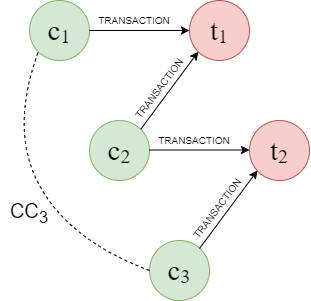
\includegraphics{images/CC3-diagram.png}
  \caption{CC3-diagram}
  \end{figure}
\item
  To compute \(CC_k(u)\), it has been mentioned that each customer
  should be traversed once only (\(u_i<>u_j\)). However, nothing has
  been mentioned for the traverse of the terminals, hence we assume that
  they can be traversed repeatedly.
\item
  In most cases, there are several transactions present among each
  customer and the connected terminals (possibly hundreds or thousands).
  To make the query more efficient, since we are only interested in
  identifying \(CC_3(u)\) relationships and not all the possible chains
  between \(u\) and \(u’\), we group our data by the start/end nodes of
  the chain and only report a single chain as a sample using
  \texttt{head(collect(...))}.
\end{itemize}

\textbf{Limitations:} Unfortunately, using the following queries for
pattern-matching, it was impossible to obtain any response even on the
50Mb database due to the shortage of memory and the complexity of the
requested pattern.

\begin{itemize}
\tightlist
\item
  \texttt{MATCH\ (c1:Customer)-{[}:TRANSACTION*4{]}-(c2:Customer)\ RETURN\ c1,\ c2}
\item
  \texttt{MATCH\ (c1:Customer)-{[}:TRANSACTION{]}-\textgreater{}(t1:Terminal)\textless{}-{[}:TRANSACTION{]}-(c2:Customer)}
  \texttt{-{[}:TRANSACTION{]}-\textgreater{}(t2:Terminal)\textless{}-{[}:TRANSACTION{]}-(c3:Customer)}
  \texttt{WHERE\ c1\ \textless{}\textgreater{}\ c2\ AND\ c1\ \textless{}\textgreater{}\ c3\ AND\ c2\ \textless{}\textgreater{}\ c3\ RETURN\ c1,\ c3}
\end{itemize}


As a result, we will report the query results and the performance
separately below with different patterns tested on a lighter database
stored in \texttt{TGtest}:

    \begin{tcolorbox}[breakable, size=fbox, boxrule=1pt, pad at break*=1mm,colback=cellbackground, colframe=cellborder]
\prompt{In}{incolor}{33}{\boxspacing}
\begin{Verbatim}[commandchars=\\\{\}]
\PY{n}{query\PYZus{}C} \PY{o}{=} \PY{l+s+s1}{\PYZsq{}\PYZsq{}\PYZsq{}}
\PY{l+s+s1}{    MATCH (c1:Customer)\PYZhy{}[:TRANSACTION]\PYZhy{}\PYZgt{}(t1:Terminal)\PYZlt{}\PYZhy{}[:TRANSACTION]\PYZhy{}(c2:Customer)\PYZhy{}[:TRANSACTION]\PYZhy{}\PYZgt{}(t2:Terminal)\PYZlt{}\PYZhy{}[:TRANSACTION]\PYZhy{}(c3:Customer)}
\PY{l+s+s1}{    WHERE c1 \PYZlt{}\PYZgt{} c2 AND c1 \PYZlt{}\PYZgt{} c3 AND c2 \PYZlt{}\PYZgt{} c3}
\PY{l+s+s1}{    WITH}
\PY{l+s+s1}{        c1,}
\PY{l+s+s1}{        c3,}
\PY{l+s+s1}{        head(collect(}\PY{l+s+s1}{\PYZob{}}
\PY{l+s+s1}{            c2: c2.customer\PYZus{}id,}
\PY{l+s+s1}{            t1: t1.terminal\PYZus{}id,}
\PY{l+s+s1}{            t2: t2.terminal\PYZus{}id\PYZcb{})}
\PY{l+s+s1}{        ) as sample\PYZus{}chain}
\PY{l+s+s1}{    RETURN}
\PY{l+s+s1}{        c1.customer\PYZus{}id AS customer,}
\PY{l+s+s1}{        c3.customer\PYZus{}id AS co\PYZus{}customer,}
\PY{l+s+s1}{            }\PY{l+s+s1}{\PYZdq{}}\PY{l+s+s1}{(c}\PY{l+s+s1}{\PYZdq{}}\PY{l+s+s1}{ + c1.customer\PYZus{}id + }\PY{l+s+s1}{\PYZdq{}}\PY{l+s+s1}{)\PYZhy{}\PYZgt{}(t}\PY{l+s+s1}{\PYZdq{}}\PY{l+s+s1}{ + sample\PYZus{}chain.t1}
\PY{l+s+s1}{            + }\PY{l+s+s1}{\PYZdq{}}\PY{l+s+s1}{)\PYZlt{}\PYZhy{}(c}\PY{l+s+s1}{\PYZdq{}}\PY{l+s+s1}{ + sample\PYZus{}chain.c2 + }\PY{l+s+s1}{\PYZdq{}}\PY{l+s+s1}{)\PYZhy{}\PYZgt{}(t}\PY{l+s+s1}{\PYZdq{}}\PY{l+s+s1}{ + sample\PYZus{}chain.t2}
\PY{l+s+s1}{            + }\PY{l+s+s1}{\PYZdq{}}\PY{l+s+s1}{)\PYZlt{}\PYZhy{}(c}\PY{l+s+s1}{\PYZdq{}}\PY{l+s+s1}{ + c3.customer\PYZus{}id + }\PY{l+s+s1}{\PYZdq{}}\PY{l+s+s1}{)}\PY{l+s+s1}{\PYZdq{}}
\PY{l+s+s1}{        AS sample\PYZus{}chain}
\PY{l+s+s1}{\PYZsq{}\PYZsq{}\PYZsq{}}
\end{Verbatim}
\end{tcolorbox}

    \begin{tcolorbox}[breakable, size=fbox, boxrule=1pt, pad at break*=1mm,colback=cellbackground, colframe=cellborder]
\prompt{In}{incolor}{34}{\boxspacing}
\begin{Verbatim}[commandchars=\\\{\}]
\PY{n}{df\PYZus{}C} \PY{o}{=} \PY{n}{db}\PY{o}{.}\PY{n}{read\PYZus{}from\PYZus{}db}\PY{p}{(}\PY{n}{query\PYZus{}C}\PY{p}{,} \PY{n}{query\PYZus{}name}\PY{o}{=}\PY{l+s+s1}{\PYZsq{}}\PY{l+s+s1}{query\PYZus{}C}\PY{l+s+s1}{\PYZsq{}}\PY{p}{,} \PY{n}{database}\PY{o}{=}\PY{l+s+s1}{\PYZsq{}}\PY{l+s+s1}{TGtest}\PY{l+s+s1}{\PYZsq{}}\PY{p}{,} \PY{n}{store\PYZus{}exec\PYZus{}time}\PY{o}{=}\PY{k+kc}{False}\PY{p}{)}
\PY{n}{df\PYZus{}C}\PY{o}{.}\PY{n}{head}\PY{p}{(}\PY{p}{)}\PY{o}{.}\PY{n}{rename}\PY{p}{(}\PY{n}{columns}\PY{o}{=}\PY{k}{lambda} \PY{n}{x}\PY{p}{:} \PY{n}{x}\PY{o}{.}\PY{n}{replace}\PY{p}{(}\PY{l+s+s1}{\PYZsq{}}\PY{l+s+s1}{\PYZus{}}\PY{l+s+s1}{\PYZsq{}}\PY{p}{,} \PY{l+s+s1}{\PYZsq{}}\PY{l+s+s1}{\PYZhy{}}\PY{l+s+s1}{\PYZsq{}}\PY{p}{)}\PY{p}{)}
\end{Verbatim}
\end{tcolorbox}

    \begin{Verbatim}[commandchars=\\\{\}]
The query returned 56 records in 3.864 s.
    \end{Verbatim}
 
            
\prompt{Out}{outcolor}{34}{}
    
    \begin{center}
\begin{tabular}{lrrl}
\toprule
 & customer & co-customer & sample-chain \\
\midrule
0 & 0 & 8 & (c0)->(t5)<-(c1)->(t3)<-(c8) \\
1 & 0 & 7 & (c0)->(t5)<-(c1)->(t3)<-(c7) \\
2 & 0 & 6 & (c0)->(t5)<-(c1)->(t3)<-(c6) \\
3 & 0 & 4 & (c0)->(t5)<-(c1)->(t7)<-(c4) \\
4 & 0 & 9 & (c0)->(t5)<-(c1)->(t0)<-(c9) \\
\bottomrule
\end{tabular}

\end{center}

    

    \begin{tcolorbox}[breakable, size=fbox, boxrule=1pt, pad at break*=1mm,colback=cellbackground, colframe=cellborder]
\prompt{In}{incolor}{35}{\boxspacing}
\begin{Verbatim}[commandchars=\\\{\}]
\PY{n}{query\PYZus{}C} \PY{o}{=} \PY{l+s+s1}{\PYZsq{}\PYZsq{}\PYZsq{}}
\PY{l+s+s1}{    MATCH (c1:Customer)\PYZhy{}[:TRANSACTION]\PYZhy{}\PYZgt{}(t1:Terminal)\PYZlt{}\PYZhy{}[:TRANSACTION]\PYZhy{}(c2:Customer)\PYZhy{}[:TRANSACTION]\PYZhy{}\PYZgt{}(t2:Terminal)\PYZlt{}\PYZhy{}[:TRANSACTION]\PYZhy{}(c3:Customer)}
\PY{l+s+s1}{    WHERE c1 \PYZlt{}\PYZgt{} c2 AND c1 \PYZlt{}\PYZgt{} c3 AND c2 \PYZlt{}\PYZgt{} c3}
\PY{l+s+s1}{    RETURN c1.customer\PYZus{}id AS customer, collect(distinct c3.customer\PYZus{}id)[0..5] as co\PYZus{}customers}
\PY{l+s+s1}{\PYZsq{}\PYZsq{}\PYZsq{}}
\end{Verbatim}
\end{tcolorbox}

    \begin{tcolorbox}[breakable, size=fbox, boxrule=1pt, pad at break*=1mm,colback=cellbackground, colframe=cellborder]
\prompt{In}{incolor}{36}{\boxspacing}
\begin{Verbatim}[commandchars=\\\{\}]
\PY{n}{df\PYZus{}C} \PY{o}{=} \PY{n}{db}\PY{o}{.}\PY{n}{read\PYZus{}from\PYZus{}db}\PY{p}{(}\PY{n}{query\PYZus{}C}\PY{p}{,} \PY{n}{query\PYZus{}name}\PY{o}{=}\PY{l+s+s1}{\PYZsq{}}\PY{l+s+s1}{query\PYZus{}C}\PY{l+s+s1}{\PYZsq{}}\PY{p}{,} \PY{n}{database}\PY{o}{=}\PY{l+s+s1}{\PYZsq{}}\PY{l+s+s1}{TGtest}\PY{l+s+s1}{\PYZsq{}}\PY{p}{,} \PY{n}{store\PYZus{}exec\PYZus{}time}\PY{o}{=}\PY{k+kc}{False}\PY{p}{)}
\PY{n}{df\PYZus{}C}\PY{o}{.}\PY{n}{head}\PY{p}{(}\PY{p}{)}\PY{o}{.}\PY{n}{rename}\PY{p}{(}\PY{n}{columns}\PY{o}{=}\PY{k}{lambda} \PY{n}{x}\PY{p}{:} \PY{n}{x}\PY{o}{.}\PY{n}{replace}\PY{p}{(}\PY{l+s+s1}{\PYZsq{}}\PY{l+s+s1}{\PYZus{}}\PY{l+s+s1}{\PYZsq{}}\PY{p}{,} \PY{l+s+s1}{\PYZsq{}}\PY{l+s+s1}{\PYZhy{}}\PY{l+s+s1}{\PYZsq{}}\PY{p}{)}\PY{p}{)}
\end{Verbatim}
\end{tcolorbox}

    \begin{Verbatim}[commandchars=\\\{\}]
The query returned 8 records in 1.951 s.
    \end{Verbatim}
 
            
\prompt{Out}{outcolor}{36}{}
    
    \begin{center}
\begin{tabular}{lrl}
\toprule
 & customer & co-customers \\
\midrule
0 & 6 & [4, 1, 7, 9, 8] \\
1 & 8 & [4, 1, 6, 7, 9] \\
2 & 1 & [4, 6, 7, 9, 8] \\
3 & 7 & [4, 1, 6, 9, 8] \\
4 & 4 & [1, 6, 7, 9, 8] \\
\bottomrule
\end{tabular}

\end{center}

    

    \begin{tcolorbox}[breakable, size=fbox, boxrule=1pt, pad at break*=1mm,colback=cellbackground, colframe=cellborder]
\prompt{In}{incolor}{37}{\boxspacing}
\begin{Verbatim}[commandchars=\\\{\}]
\PY{n}{query\PYZus{}C} \PY{o}{=} \PY{l+s+s1}{\PYZsq{}\PYZsq{}\PYZsq{}}
\PY{l+s+s1}{    MATCH (c:Customer)\PYZhy{}[t:TRANSACTION]\PYZhy{}\PYZgt{}(tm:Terminal)}
\PY{l+s+s1}{    WITH c, tm, head(collect(t)) as t}
\PY{l+s+s1}{    WITH collect(}\PY{l+s+s1}{\PYZob{}}
\PY{l+s+s1}{        c:c.customer\PYZus{}id, t:t.transaction\PYZus{}id, tm:tm.terminal\PYZus{}id}
\PY{l+s+s1}{    \PYZcb{}) as summarized\PYZus{}graph}
\PY{l+s+s1}{    UNWIND summarized\PYZus{}graph AS depth1}
\PY{l+s+s1}{    UNWIND summarized\PYZus{}graph AS depth2}
\PY{l+s+s1}{    UNWIND summarized\PYZus{}graph AS depth3}
\PY{l+s+s1}{    UNWIND summarized\PYZus{}graph AS depth4}
\PY{l+s+s1}{    WITH}
\PY{l+s+s1}{        depth1.c AS c1, depth1.t AS t1, depth1.tm AS tm1,}
\PY{l+s+s1}{        depth2.c AS c2, depth2.t AS t2, depth2.tm AS tm2,}
\PY{l+s+s1}{        depth3.c AS c3, depth3.t AS t3, depth3.tm AS tm3,}
\PY{l+s+s1}{        depth4.c AS c4, depth4.t AS t4, depth4.tm AS tm4}
\PY{l+s+s1}{    WHERE}
\PY{l+s+s1}{        tm1=tm2 AND tm3=tm4 AND c2=c3}
\PY{l+s+s1}{        AND c1\PYZlt{}\PYZgt{}c2 AND c1\PYZlt{}\PYZgt{}c4 AND c2\PYZlt{}\PYZgt{}c4}
\PY{l+s+s1}{    RETURN}
\PY{l+s+s1}{        c1 AS customer,}
\PY{l+s+s1}{        c4 AS co\PYZus{}customer,}
\PY{l+s+s1}{            }\PY{l+s+s1}{\PYZdq{}}\PY{l+s+s1}{(c}\PY{l+s+s1}{\PYZdq{}}\PY{l+s+s1}{ + c1 + }\PY{l+s+s1}{\PYZdq{}}\PY{l+s+s1}{)\PYZhy{}\PYZgt{}(t}\PY{l+s+s1}{\PYZdq{}}\PY{l+s+s1}{ + tm1}
\PY{l+s+s1}{            + }\PY{l+s+s1}{\PYZdq{}}\PY{l+s+s1}{)\PYZlt{}\PYZhy{}(c}\PY{l+s+s1}{\PYZdq{}}\PY{l+s+s1}{ + c2 + }\PY{l+s+s1}{\PYZdq{}}\PY{l+s+s1}{)\PYZhy{}\PYZgt{}(t}\PY{l+s+s1}{\PYZdq{}}\PY{l+s+s1}{ + tm3}
\PY{l+s+s1}{            + }\PY{l+s+s1}{\PYZdq{}}\PY{l+s+s1}{)\PYZlt{}\PYZhy{}(c}\PY{l+s+s1}{\PYZdq{}}\PY{l+s+s1}{ + c4 + }\PY{l+s+s1}{\PYZdq{}}\PY{l+s+s1}{)}\PY{l+s+s1}{\PYZdq{}}
\PY{l+s+s1}{        AS sample\PYZus{}chain}
\PY{l+s+s1}{\PYZsq{}\PYZsq{}\PYZsq{}}
\end{Verbatim}
\end{tcolorbox}

    \begin{tcolorbox}[breakable, size=fbox, boxrule=1pt, pad at break*=1mm,colback=cellbackground, colframe=cellborder]
\prompt{In}{incolor}{38}{\boxspacing}
\begin{Verbatim}[commandchars=\\\{\}]
\PY{n}{df\PYZus{}C} \PY{o}{=} \PY{n}{db}\PY{o}{.}\PY{n}{read\PYZus{}from\PYZus{}db}\PY{p}{(}\PY{n}{query\PYZus{}C}\PY{p}{,} \PY{n}{query\PYZus{}name}\PY{o}{=}\PY{l+s+s1}{\PYZsq{}}\PY{l+s+s1}{query\PYZus{}C}\PY{l+s+s1}{\PYZsq{}}\PY{p}{,} \PY{n}{database}\PY{o}{=}\PY{l+s+s1}{\PYZsq{}}\PY{l+s+s1}{TGtest}\PY{l+s+s1}{\PYZsq{}}\PY{p}{,} \PY{n}{store\PYZus{}exec\PYZus{}time}\PY{o}{=}\PY{k+kc}{False}\PY{p}{)}
\PY{n}{df\PYZus{}C}\PY{o}{.}\PY{n}{head}\PY{p}{(}\PY{p}{)}\PY{o}{.}\PY{n}{rename}\PY{p}{(}\PY{n}{columns}\PY{o}{=}\PY{k}{lambda} \PY{n}{x}\PY{p}{:} \PY{n}{x}\PY{o}{.}\PY{n}{replace}\PY{p}{(}\PY{l+s+s1}{\PYZsq{}}\PY{l+s+s1}{\PYZus{}}\PY{l+s+s1}{\PYZsq{}}\PY{p}{,} \PY{l+s+s1}{\PYZsq{}}\PY{l+s+s1}{\PYZhy{}}\PY{l+s+s1}{\PYZsq{}}\PY{p}{)}\PY{p}{)}
\end{Verbatim}
\end{tcolorbox}

    \begin{Verbatim}[commandchars=\\\{\}]
The query returned 7310 records in 2.282 s.
    \end{Verbatim}
 
            
\prompt{Out}{outcolor}{38}{}
    
    \begin{center}
\begin{tabular}{lrrl}
\toprule
 & customer & co-customer & sample-chain \\
\midrule
0 & 0 & 6 & (c0)->(t5)<-(c1)->(t3)<-(c6) \\
1 & 0 & 7 & (c0)->(t5)<-(c1)->(t3)<-(c7) \\
2 & 0 & 8 & (c0)->(t5)<-(c1)->(t3)<-(c8) \\
3 & 0 & 4 & (c0)->(t5)<-(c1)->(t7)<-(c4) \\
4 & 0 & 6 & (c0)->(t5)<-(c1)->(t7)<-(c6) \\
\bottomrule
\end{tabular}

\end{center}

    

    As mentioned in the limitations, none of the queries above were capable
of performing well on the scaled versions of the databases. The reason
is, that there might be thousands of transactions between each customer
and terminal, and directly applying the \texttt{MATCH} operation on the
whole graph explodes, and also summarizing along with pattern-matching
in the same query was reluctant to provide fast response. Therefore, we
will proceed with another technique, described below:

\begin{itemize}
\tightlist
\item
  First, for each customer and terminal, if they are connected, we add a
  single new relationship between them labeled \texttt{:CONNECTED}.
\item
  Then, instead of performing pattern-matching on
  \texttt{()-{[}:TRANSACTION{]}-()}, we will instead use
  \texttt{()-{[}:CONNECTED{]}-()} which will substantially decrease the
  runtime.
\item
  The rest of the queries will be organized similarly as before.
\end{itemize}

    \begin{tcolorbox}[breakable, size=fbox, boxrule=1pt, pad at break*=1mm,colback=cellbackground, colframe=cellborder]
\prompt{In}{incolor}{39}{\boxspacing}
\begin{Verbatim}[commandchars=\\\{\}]
\PY{n}{query\PYZus{}C} \PY{o}{=} \PY{l+s+s1}{\PYZsq{}\PYZsq{}\PYZsq{}}
\PY{l+s+s1}{    CALL apoc.periodic.iterate(}
\PY{l+s+s1}{        }\PY{l+s+s1}{\PYZdq{}}\PY{l+s+s1}{MATCH (c:Customer)\PYZhy{}[t:TRANSACTION]\PYZhy{}\PYZgt{}(tm:Terminal)}
\PY{l+s+s1}{        RETURN c, tm, count(t) as t}\PY{l+s+s1}{\PYZdq{}}\PY{l+s+s1}{,}
\PY{l+s+s1}{        }\PY{l+s+s1}{\PYZdq{}}\PY{l+s+s1}{MERGE (c)\PYZhy{}[:CONNECTED]\PYZhy{}\PYZgt{}(tm)}\PY{l+s+s1}{\PYZdq{}}\PY{l+s+s1}{,}
\PY{l+s+s1}{        }\PY{l+s+s1}{\PYZob{}}\PY{l+s+s1}{batchSize:1000, iterateList:true\PYZcb{}}
\PY{l+s+s1}{    );}
\PY{l+s+s1}{\PYZsq{}\PYZsq{}\PYZsq{}}
\end{Verbatim}
\end{tcolorbox}

    \begin{tcolorbox}[breakable, size=fbox, boxrule=1pt, pad at break*=1mm,colback=cellbackground, colframe=cellborder]
\prompt{In}{incolor}{40}{\boxspacing}
\begin{Verbatim}[commandchars=\\\{\}]
\PY{n}{\PYZus{}} \PY{o}{=} \PY{n}{db}\PY{o}{.}\PY{n}{read\PYZus{}from\PYZus{}db}\PY{p}{(}\PY{n}{query\PYZus{}C}\PY{p}{,} \PY{n}{query\PYZus{}name}\PY{o}{=}\PY{l+s+s1}{\PYZsq{}}\PY{l+s+s1}{query\PYZus{}C}\PY{l+s+s1}{\PYZsq{}}\PY{p}{,} \PY{n}{database}\PY{o}{=}\PY{l+s+s1}{\PYZsq{}}\PY{l+s+s1}{TG50}\PY{l+s+s1}{\PYZsq{}}\PY{p}{)}
\PY{n}{\PYZus{}} \PY{o}{=} \PY{n}{db}\PY{o}{.}\PY{n}{read\PYZus{}from\PYZus{}db}\PY{p}{(}\PY{n}{query\PYZus{}C}\PY{p}{,} \PY{n}{query\PYZus{}name}\PY{o}{=}\PY{l+s+s1}{\PYZsq{}}\PY{l+s+s1}{query\PYZus{}C}\PY{l+s+s1}{\PYZsq{}}\PY{p}{,} \PY{n}{database}\PY{o}{=}\PY{l+s+s1}{\PYZsq{}}\PY{l+s+s1}{TG100}\PY{l+s+s1}{\PYZsq{}}\PY{p}{)}
\PY{n}{\PYZus{}} \PY{o}{=} \PY{n}{db}\PY{o}{.}\PY{n}{read\PYZus{}from\PYZus{}db}\PY{p}{(}\PY{n}{query\PYZus{}C}\PY{p}{,} \PY{n}{query\PYZus{}name}\PY{o}{=}\PY{l+s+s1}{\PYZsq{}}\PY{l+s+s1}{query\PYZus{}C}\PY{l+s+s1}{\PYZsq{}}\PY{p}{,} \PY{n}{database}\PY{o}{=}\PY{l+s+s1}{\PYZsq{}}\PY{l+s+s1}{TG200}\PY{l+s+s1}{\PYZsq{}}\PY{p}{)}
\end{Verbatim}
\end{tcolorbox}

    \begin{Verbatim}[commandchars=\\\{\}]
The query returned 1 records in 0.957 s.
The query returned 1 records in 1.016 s.
The query returned 1 records in 1.768 s.
    \end{Verbatim}

    As we can see, the operation above is very fast. Now, we can easily
query the chain of our interest using the \texttt{CONNECTED}
relationships.

    \begin{tcolorbox}[breakable, size=fbox, boxrule=1pt, pad at break*=1mm,colback=cellbackground, colframe=cellborder]
\prompt{In}{incolor}{41}{\boxspacing}
\begin{Verbatim}[commandchars=\\\{\}]
\PY{n}{quer\PYZus{}C\PYZus{}read} \PY{o}{=} \PY{l+s+s1}{\PYZsq{}\PYZsq{}\PYZsq{}}
\PY{l+s+s1}{    MATCH (c1:Customer)\PYZhy{}[:CONNECTED]\PYZhy{}\PYZgt{}(t1:Terminal)\PYZlt{}\PYZhy{}[:CONNECTED]\PYZhy{}(c2:Customer)\PYZhy{}[:CONNECTED]\PYZhy{}\PYZgt{}(t2:Terminal)\PYZlt{}\PYZhy{}[:CONNECTED]\PYZhy{}(c3:Customer)}
\PY{l+s+s1}{    WHERE c1 \PYZlt{}\PYZgt{} c2 AND c1 \PYZlt{}\PYZgt{} c3 AND c2 \PYZlt{}\PYZgt{} c3}
\PY{l+s+s1}{    RETURN}
\PY{l+s+s1}{        c1.customer\PYZus{}id AS customer,}
\PY{l+s+s1}{        c3.customer\PYZus{}id AS co\PYZus{}customer,}
\PY{l+s+s1}{            }\PY{l+s+s1}{\PYZdq{}}\PY{l+s+s1}{(c}\PY{l+s+s1}{\PYZdq{}}\PY{l+s+s1}{ + c1.customer\PYZus{}id + }\PY{l+s+s1}{\PYZdq{}}\PY{l+s+s1}{)\PYZhy{}\PYZgt{}(t}\PY{l+s+s1}{\PYZdq{}}\PY{l+s+s1}{ + t1.terminal\PYZus{}id}
\PY{l+s+s1}{            + }\PY{l+s+s1}{\PYZdq{}}\PY{l+s+s1}{)\PYZlt{}\PYZhy{}(c}\PY{l+s+s1}{\PYZdq{}}\PY{l+s+s1}{ + c2.customer\PYZus{}id + }\PY{l+s+s1}{\PYZdq{}}\PY{l+s+s1}{)\PYZhy{}\PYZgt{}(t}\PY{l+s+s1}{\PYZdq{}}\PY{l+s+s1}{ + t2.terminal\PYZus{}id}
\PY{l+s+s1}{            + }\PY{l+s+s1}{\PYZdq{}}\PY{l+s+s1}{)\PYZlt{}\PYZhy{}(c}\PY{l+s+s1}{\PYZdq{}}\PY{l+s+s1}{ + c3.customer\PYZus{}id + }\PY{l+s+s1}{\PYZdq{}}\PY{l+s+s1}{)}\PY{l+s+s1}{\PYZdq{}}
\PY{l+s+s1}{        AS sample\PYZus{}chain}
\PY{l+s+s1}{    LIMIT 5}
\PY{l+s+s1}{\PYZsq{}\PYZsq{}\PYZsq{}}
\end{Verbatim}
\end{tcolorbox}

    \begin{tcolorbox}[breakable, size=fbox, boxrule=1pt, pad at break*=1mm,colback=cellbackground, colframe=cellborder]
\prompt{In}{incolor}{42}{\boxspacing}
\begin{Verbatim}[commandchars=\\\{\}]
\PY{n}{df\PYZus{}C\PYZus{}50} \PY{o}{=} \PY{n}{db}\PY{o}{.}\PY{n}{read\PYZus{}from\PYZus{}db}\PY{p}{(}\PY{n}{quer\PYZus{}C\PYZus{}read}\PY{p}{,} \PY{n}{query\PYZus{}name}\PY{o}{=}\PY{l+s+s1}{\PYZsq{}}\PY{l+s+s1}{query\PYZus{}C}\PY{l+s+s1}{\PYZsq{}}\PY{p}{,} \PY{n}{database}\PY{o}{=}\PY{l+s+s1}{\PYZsq{}}\PY{l+s+s1}{TG50}\PY{l+s+s1}{\PYZsq{}}\PY{p}{,} \PY{n}{store\PYZus{}exec\PYZus{}time}\PY{o}{=}\PY{k+kc}{False}\PY{p}{)}
\PY{n}{df\PYZus{}C\PYZus{}100} \PY{o}{=} \PY{n}{db}\PY{o}{.}\PY{n}{read\PYZus{}from\PYZus{}db}\PY{p}{(}\PY{n}{quer\PYZus{}C\PYZus{}read}\PY{p}{,} \PY{n}{query\PYZus{}name}\PY{o}{=}\PY{l+s+s1}{\PYZsq{}}\PY{l+s+s1}{query\PYZus{}C}\PY{l+s+s1}{\PYZsq{}}\PY{p}{,} \PY{n}{database}\PY{o}{=}\PY{l+s+s1}{\PYZsq{}}\PY{l+s+s1}{TG100}\PY{l+s+s1}{\PYZsq{}}\PY{p}{,} \PY{n}{store\PYZus{}exec\PYZus{}time}\PY{o}{=}\PY{k+kc}{False}\PY{p}{)}
\PY{n}{df\PYZus{}C\PYZus{}200} \PY{o}{=} \PY{n}{db}\PY{o}{.}\PY{n}{read\PYZus{}from\PYZus{}db}\PY{p}{(}\PY{n}{quer\PYZus{}C\PYZus{}read}\PY{p}{,} \PY{n}{query\PYZus{}name}\PY{o}{=}\PY{l+s+s1}{\PYZsq{}}\PY{l+s+s1}{query\PYZus{}C}\PY{l+s+s1}{\PYZsq{}}\PY{p}{,} \PY{n}{database}\PY{o}{=}\PY{l+s+s1}{\PYZsq{}}\PY{l+s+s1}{TG200}\PY{l+s+s1}{\PYZsq{}}\PY{p}{,} \PY{n}{store\PYZus{}exec\PYZus{}time}\PY{o}{=}\PY{k+kc}{False}\PY{p}{)}
\end{Verbatim}
\end{tcolorbox}

    \begin{Verbatim}[commandchars=\\\{\}]
The query returned 5 records in 0.3 s.
The query returned 5 records in 0.208 s.
The query returned 5 records in 0.205 s.
    \end{Verbatim}

    \begin{tcolorbox}[breakable, size=fbox, boxrule=1pt, pad at break*=1mm,colback=cellbackground, colframe=cellborder]
\prompt{In}{incolor}{43}{\boxspacing}
\begin{Verbatim}[commandchars=\\\{\}]
\PY{n}{df\PYZus{}C\PYZus{}50}\PY{o}{.}\PY{n}{head}\PY{p}{(}\PY{p}{)}\PY{o}{.}\PY{n}{rename}\PY{p}{(}\PY{n}{columns}\PY{o}{=}\PY{k}{lambda} \PY{n}{x}\PY{p}{:} \PY{n}{x}\PY{o}{.}\PY{n}{replace}\PY{p}{(}\PY{l+s+s1}{\PYZsq{}}\PY{l+s+s1}{\PYZus{}}\PY{l+s+s1}{\PYZsq{}}\PY{p}{,} \PY{l+s+s1}{\PYZsq{}}\PY{l+s+s1}{\PYZhy{}}\PY{l+s+s1}{\PYZsq{}}\PY{p}{)}\PY{p}{)}
\end{Verbatim}
\end{tcolorbox}
 
            
\prompt{Out}{outcolor}{43}{}
    
    \begin{center}
\begin{tabular}{lrrl}
\toprule
 & customer & co-customer & sample-chain \\
\midrule
0 & 399 & 1 & (c399)->(t0)<-(c337)->(t5)<-(c1) \\
1 & 399 & 1 & (c399)->(t0)<-(c337)->(t378)<-(c1) \\
2 & 337 & 1 & (c337)->(t0)<-(c399)->(t5)<-(c1) \\
3 & 337 & 1 & (c337)->(t0)<-(c399)->(t378)<-(c1) \\
4 & 337 & 385 & (c337)->(t0)<-(c399)->(t270)<-(c385) \\
\bottomrule
\end{tabular}

\end{center}

    

    \hypertarget{query-d}{%
\subsubsection{Query (D)}\label{query-d}}

    \textbf{Query:} Extend the logical model that you have stored in the
NOSQL database by introducing the following information:

\begin{enumerate}
\def\labelenumi{\arabic{enumi}.}
\tightlist
\item
  Each transaction should be extended with:

  \begin{itemize}
  \tightlist
  \item
    The period of the day \{morning, afternoon, evening, night\} in
    which the transaction has been executed.
  \item
    The kind of products that have been bought through the transaction
    \{hightech, food, clothing, consumable, other\}
  \item
    The feeling of security expressed by the user. This is an integer
    value between 1 and 5 expressed by the user when conclude the
    transaction. The values can be chosen randomly.
  \end{itemize}
\item
  Customers that make more than three transactions from the same
  terminal expressing a similar average feeling of security should be
  connected as ``buying\_friends''. Therefore also this kind of
  relationship should be explicitly stored in the NOSQL database and can
  be queried. Note, two average feelings of security are considered
  similar when their difference is lower than 1.
\end{enumerate}

We will proceed with each of the steps separately, distributing to
queries \texttt{D1} and \texttt{D2} for the above tasks.

    \textbf{Assumptions:}

\begin{itemize}
\tightlist
\item
  To obtain the period of the day, we utilize the transaction hours such
  that transactions within ``00:00-06:00'' are tagged ``night'',
  ``06:00-12:00'' as ``morning'', ``12:00-18:00'' as ``afternoon'', and
  ``18:00-00:00'' as ``evening''.
\item
  For the kind of product purchased along the transaction, we assume
  that the products only belong to a single category among
  \{``high-tech'', ``food'', ``clothing'', ``consumable'', ``other''\},
  which we randomly select and assign to each transaction. If we instead
  wanted to have a \emph{list} of products for each transaction, we
  could create a list such that each entry (corresponding to a product)
  is randomly included or excluded. For example,
  \texttt{CASE\ WHEN\ rand()\textless{}0.5\ THEN\ "high-tech"\ END}, and
  we repeat the same for all other products.
\item
  Security feeling of the transaction is also drawn randomly and
  distributed as an integer number from 1 to 5.
\end{itemize}

    \hypertarget{query-d1}{%
\paragraph{Query (D1)}\label{query-d1}}

    At first, the below query was used to update the transactions with a new
set of values.

    \begin{tcolorbox}[breakable, size=fbox, boxrule=1pt, pad at break*=1mm,colback=cellbackground, colframe=cellborder]
\prompt{In}{incolor}{44}{\boxspacing}
\begin{Verbatim}[commandchars=\\\{\}]
\PY{n}{query\PYZus{}D1} \PY{o}{=} \PY{l+s+s1}{\PYZsq{}\PYZsq{}\PYZsq{}}
\PY{l+s+s1}{    MATCH (:Customer)\PYZhy{}[t:TRANSACTION]\PYZhy{}\PYZgt{}(:Terminal)}
\PY{l+s+s1}{    SET}
\PY{l+s+s1}{        t.period\PYZus{}of\PYZus{}day = }
\PY{l+s+s1}{            CASE}
\PY{l+s+s1}{                WHEN datetime(t.tx\PYZus{}datetime).hour \PYZgt{}= 6 AND datetime(t.tx\PYZus{}datetime).hour \PYZlt{} 12 THEN }\PY{l+s+s1}{\PYZsq{}}\PY{l+s+s1}{morning}\PY{l+s+s1}{\PYZsq{}}
\PY{l+s+s1}{                WHEN datetime(t.tx\PYZus{}datetime).hour \PYZgt{}= 12 AND datetime(t.tx\PYZus{}datetime).hour \PYZlt{} 18 THEN }\PY{l+s+s1}{\PYZsq{}}\PY{l+s+s1}{afternoon}\PY{l+s+s1}{\PYZsq{}}
\PY{l+s+s1}{                WHEN datetime(t.tx\PYZus{}datetime).hour \PYZgt{}= 18 AND datetime(t.tx\PYZus{}datetime).hour \PYZlt{} 24 THEN }\PY{l+s+s1}{\PYZsq{}}\PY{l+s+s1}{evening}\PY{l+s+s1}{\PYZsq{}}
\PY{l+s+s1}{                ELSE }\PY{l+s+s1}{\PYZsq{}}\PY{l+s+s1}{night}\PY{l+s+s1}{\PYZsq{}}
\PY{l+s+s1}{            END,}
\PY{l+s+s1}{        t.product = }
\PY{l+s+s1}{            [}\PY{l+s+s1}{\PYZdq{}}\PY{l+s+s1}{high\PYZhy{}tech}\PY{l+s+s1}{\PYZdq{}}\PY{l+s+s1}{, }\PY{l+s+s1}{\PYZdq{}}\PY{l+s+s1}{food}\PY{l+s+s1}{\PYZdq{}}\PY{l+s+s1}{, }\PY{l+s+s1}{\PYZdq{}}\PY{l+s+s1}{clothing}\PY{l+s+s1}{\PYZdq{}}\PY{l+s+s1}{, }\PY{l+s+s1}{\PYZdq{}}\PY{l+s+s1}{consumable}\PY{l+s+s1}{\PYZdq{}}\PY{l+s+s1}{, }\PY{l+s+s1}{\PYZdq{}}\PY{l+s+s1}{other}\PY{l+s+s1}{\PYZdq{}}\PY{l+s+s1}{]}
\PY{l+s+s1}{            [toInteger(round(rand() * 4))],}
\PY{l+s+s1}{        t.security\PYZus{}feeling = toInteger(round(rand() * 4) + 1)}

\PY{l+s+s1}{    RETURN}
\PY{l+s+s1}{        t.transaction\PYZus{}id, t.customer\PYZus{}id, t.terminal\PYZus{}id, t.tx\PYZus{}datetime,}
\PY{l+s+s1}{        t.period\PYZus{}of\PYZus{}day, t.product, t.security\PYZus{}feeling}
\PY{l+s+s1}{    LIMIT 5}
\PY{l+s+s1}{\PYZsq{}\PYZsq{}\PYZsq{}}
\end{Verbatim}
\end{tcolorbox}

    The query above, however, failed to provide fast responses as the
dataset scaled. To overcome this issue, we optimized the query and
utilized \texttt{CALL\ apoc.periodic.iterate} to improve the performance
by parallelization and batching. We will now try to obtain the same
result without using \texttt{CASE} expressions, using array indexing
techniques, to check whether it improves the performance of the query or
not.

    \begin{tcolorbox}[breakable, size=fbox, boxrule=1pt, pad at break*=1mm,colback=cellbackground, colframe=cellborder]
\prompt{In}{incolor}{45}{\boxspacing}
\begin{Verbatim}[commandchars=\\\{\}]
\PY{n}{query\PYZus{}D1} \PY{o}{=} \PY{l+s+s1}{\PYZsq{}\PYZsq{}\PYZsq{}}
\PY{l+s+s1}{    CALL apoc.periodic.iterate(}
\PY{l+s+s1}{        }\PY{l+s+s1}{\PYZdq{}}\PY{l+s+s1}{MATCH (:Customer)\PYZhy{}[t:TRANSACTION]\PYZhy{}\PYZgt{}(:Terminal)}
\PY{l+s+s1}{        RETURN t, datetime(t.tx\PYZus{}datetime).hour/6 AS period\PYZus{}index, toInteger(round(rand()*4)) AS random\PYZus{}index}\PY{l+s+s1}{\PYZdq{}}\PY{l+s+s1}{,}
\PY{l+s+s1}{        }\PY{l+s+s1}{\PYZdq{}}\PY{l+s+s1}{SET}
\PY{l+s+s1}{            t.period\PYZus{}of\PYZus{}day = [}\PY{l+s+s1}{\PYZsq{}}\PY{l+s+s1}{night}\PY{l+s+s1}{\PYZsq{}}\PY{l+s+s1}{, }\PY{l+s+s1}{\PYZsq{}}\PY{l+s+s1}{morning}\PY{l+s+s1}{\PYZsq{}}\PY{l+s+s1}{, }\PY{l+s+s1}{\PYZsq{}}\PY{l+s+s1}{afternoon}\PY{l+s+s1}{\PYZsq{}}\PY{l+s+s1}{, }\PY{l+s+s1}{\PYZsq{}}\PY{l+s+s1}{evening}\PY{l+s+s1}{\PYZsq{}}\PY{l+s+s1}{][period\PYZus{}index],}
\PY{l+s+s1}{            t.product = [}\PY{l+s+s1}{\PYZsq{}}\PY{l+s+s1}{high\PYZhy{}tech}\PY{l+s+s1}{\PYZsq{}}\PY{l+s+s1}{, }\PY{l+s+s1}{\PYZsq{}}\PY{l+s+s1}{food}\PY{l+s+s1}{\PYZsq{}}\PY{l+s+s1}{, }\PY{l+s+s1}{\PYZsq{}}\PY{l+s+s1}{clothing}\PY{l+s+s1}{\PYZsq{}}\PY{l+s+s1}{, }\PY{l+s+s1}{\PYZsq{}}\PY{l+s+s1}{consumable}\PY{l+s+s1}{\PYZsq{}}\PY{l+s+s1}{, }\PY{l+s+s1}{\PYZsq{}}\PY{l+s+s1}{other}\PY{l+s+s1}{\PYZsq{}}\PY{l+s+s1}{][random\PYZus{}index],}
\PY{l+s+s1}{            t.security\PYZus{}feeling = random\PYZus{}index + 1}\PY{l+s+s1}{\PYZdq{}}\PY{l+s+s1}{,}
\PY{l+s+s1}{      }\PY{l+s+s1}{\PYZob{}}\PY{l+s+s1}{batchSize:1000, iterateList:true\PYZcb{}}
\PY{l+s+s1}{    );}
\PY{l+s+s1}{\PYZsq{}\PYZsq{}\PYZsq{}}
\end{Verbatim}
\end{tcolorbox}

    \begin{tcolorbox}[breakable, size=fbox, boxrule=1pt, pad at break*=1mm,colback=cellbackground, colframe=cellborder]
\prompt{In}{incolor}{46}{\boxspacing}
\begin{Verbatim}[commandchars=\\\{\}]
\PY{n}{\PYZus{}} \PY{o}{=} \PY{n}{db}\PY{o}{.}\PY{n}{read\PYZus{}from\PYZus{}db}\PY{p}{(}\PY{n}{query\PYZus{}D1}\PY{p}{,} \PY{n}{query\PYZus{}name}\PY{o}{=}\PY{l+s+s1}{\PYZsq{}}\PY{l+s+s1}{query\PYZus{}D1}\PY{l+s+s1}{\PYZsq{}}\PY{p}{,} \PY{n}{database}\PY{o}{=}\PY{l+s+s1}{\PYZsq{}}\PY{l+s+s1}{TG50}\PY{l+s+s1}{\PYZsq{}}\PY{p}{)}
\PY{n}{\PYZus{}} \PY{o}{=} \PY{n}{db}\PY{o}{.}\PY{n}{read\PYZus{}from\PYZus{}db}\PY{p}{(}\PY{n}{query\PYZus{}D1}\PY{p}{,} \PY{n}{query\PYZus{}name}\PY{o}{=}\PY{l+s+s1}{\PYZsq{}}\PY{l+s+s1}{query\PYZus{}D1}\PY{l+s+s1}{\PYZsq{}}\PY{p}{,} \PY{n}{database}\PY{o}{=}\PY{l+s+s1}{\PYZsq{}}\PY{l+s+s1}{TG100}\PY{l+s+s1}{\PYZsq{}}\PY{p}{)}
\PY{n}{\PYZus{}} \PY{o}{=} \PY{n}{db}\PY{o}{.}\PY{n}{read\PYZus{}from\PYZus{}db}\PY{p}{(}\PY{n}{query\PYZus{}D1}\PY{p}{,} \PY{n}{query\PYZus{}name}\PY{o}{=}\PY{l+s+s1}{\PYZsq{}}\PY{l+s+s1}{query\PYZus{}D1}\PY{l+s+s1}{\PYZsq{}}\PY{p}{,} \PY{n}{database}\PY{o}{=}\PY{l+s+s1}{\PYZsq{}}\PY{l+s+s1}{TG200}\PY{l+s+s1}{\PYZsq{}}\PY{p}{)}
\end{Verbatim}
\end{tcolorbox}

    \begin{Verbatim}[commandchars=\\\{\}]
The query returned 1 records in 8.12 s.
The query returned 1 records in 10.959 s.
The query returned 1 records in 21.91 s.
    \end{Verbatim}

    As an example, we will now report the first 5 transactions with the
updated properties:

    \begin{tcolorbox}[breakable, size=fbox, boxrule=1pt, pad at break*=1mm,colback=cellbackground, colframe=cellborder]
\prompt{In}{incolor}{47}{\boxspacing}
\begin{Verbatim}[commandchars=\\\{\}]
\PY{n}{query\PYZus{}D1\PYZus{}read} \PY{o}{=} \PY{l+s+s1}{\PYZsq{}\PYZsq{}\PYZsq{}}
\PY{l+s+s1}{    MATCH (:Customer)\PYZhy{}[t:TRANSACTION]\PYZhy{}\PYZgt{}(:Terminal)}
\PY{l+s+s1}{    RETURN}
\PY{l+s+s1}{        t.transaction\PYZus{}id, t.customer\PYZus{}id, t.terminal\PYZus{}id, t.tx\PYZus{}datetime,}
\PY{l+s+s1}{        t.period\PYZus{}of\PYZus{}day, t.product, t.security\PYZus{}feeling}
\PY{l+s+s1}{    LIMIT 5}
\PY{l+s+s1}{\PYZsq{}\PYZsq{}\PYZsq{}}
\end{Verbatim}
\end{tcolorbox}

    \begin{tcolorbox}[breakable, size=fbox, boxrule=1pt, pad at break*=1mm,colback=cellbackground, colframe=cellborder]
\prompt{In}{incolor}{48}{\boxspacing}
\begin{Verbatim}[commandchars=\\\{\}]
\PY{n}{df\PYZus{}D1} \PY{o}{=} \PY{n}{db}\PY{o}{.}\PY{n}{read\PYZus{}from\PYZus{}db}\PY{p}{(}\PY{n}{query\PYZus{}D1\PYZus{}read}\PY{p}{,} \PY{n}{query\PYZus{}name}\PY{o}{=}\PY{l+s+s1}{\PYZsq{}}\PY{l+s+s1}{query\PYZus{}D1}\PY{l+s+s1}{\PYZsq{}}\PY{p}{,} \PY{n}{database}\PY{o}{=}\PY{l+s+s1}{\PYZsq{}}\PY{l+s+s1}{TG50}\PY{l+s+s1}{\PYZsq{}}\PY{p}{,} \PY{n}{store\PYZus{}exec\PYZus{}time}\PY{o}{=}\PY{k+kc}{False}\PY{p}{)}
\PY{n}{df\PYZus{}D1}\PY{o}{.}\PY{n}{rename}\PY{p}{(}\PY{n}{columns}\PY{o}{=}\PY{k}{lambda} \PY{n}{x}\PY{p}{:} \PY{n}{x}\PY{o}{.}\PY{n}{replace}\PY{p}{(}\PY{l+s+s1}{\PYZsq{}}\PY{l+s+s1}{\PYZus{}}\PY{l+s+s1}{\PYZsq{}}\PY{p}{,} \PY{l+s+s1}{\PYZsq{}}\PY{l+s+s1}{\PYZhy{}}\PY{l+s+s1}{\PYZsq{}}\PY{p}{)}\PY{p}{)}
\end{Verbatim}
\end{tcolorbox}

    \begin{Verbatim}[commandchars=\\\{\}]
The query returned 5 records in 0.099 s.
    \end{Verbatim}
 
            
\prompt{Out}{outcolor}{48}{}
    
    \begin{center}
\footnotesize
\begin{tabular}{lrrrlllr}
\toprule
 & t.transaction-id & t.customer-id & t.terminal-id & t.tx-datetime & t.period-of-day & t.product & t.security-feeling \\
\midrule
0 & 90003 & 399 & 0 & 2018-07-24T06:11:36.000000000 & morning & clothing & 3 \\
1 & 287621 & 337 & 0 & 2019-03-31T18:59:28.000000000 & evening & food & 2 \\
2 & 285340 & 337 & 0 & 2019-03-29T01:25:16.000000000 & night & clothing & 3 \\
3 & 284817 & 337 & 0 & 2019-03-28T09:33:46.000000000 & morning & food & 2 \\
4 & 281994 & 399 & 0 & 2019-03-24T16:22:42.000000000 & afternoon & clothing & 3 \\
\bottomrule
\end{tabular}

\end{center}

    

    \hypertarget{query-d2}{%
\paragraph{Query (D2)}\label{query-d2}}

    In a separate query, we attempt to add \texttt{BUYING\_FRIEND}
relationships. We find customers with +3 transactions on the same
terminal, computing their average security feeling separately, and
connect them if their feelings is similar.

\begin{figure}
\centering
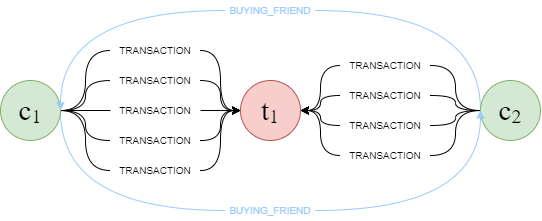
\includegraphics{images/buying-friends-diagram.png}
\caption{buying\_friends}
\end{figure}

At first, the query below was provided the insert the additional
\texttt{BUYING\_FRIEND} relationships in the database.

    \begin{tcolorbox}[breakable, size=fbox, boxrule=1pt, pad at break*=1mm,colback=cellbackground, colframe=cellborder]
\prompt{In}{incolor}{49}{\boxspacing}
\begin{Verbatim}[commandchars=\\\{\}]
\PY{n}{query\PYZus{}D2} \PY{o}{=} \PY{l+s+s1}{\PYZsq{}\PYZsq{}\PYZsq{}}
\PY{l+s+s1}{    MATCH (c1:Customer)\PYZhy{}[t1:TRANSACTION]\PYZhy{}\PYZgt{}(tm1:Terminal)}
\PY{l+s+s1}{    WITH c1, tm1, COUNT(t1) AS n\PYZus{}transactions\PYZus{}c1, avg(t1.security\PYZus{}feeling) AS avg\PYZus{}security\PYZus{}t1}
\PY{l+s+s1}{    WHERE n\PYZus{}transactions\PYZus{}c1 \PYZgt{} 3}
\PY{l+s+s1}{    }
\PY{l+s+s1}{    MATCH (c2:Customer)\PYZhy{}[t2:TRANSACTION]\PYZhy{}\PYZgt{}(tm2:Terminal)}
\PY{l+s+s1}{    WITH c2, tm2, COUNT(t2) AS n\PYZus{}transactions\PYZus{}c2, avg(t2.security\PYZus{}feeling) AS avg\PYZus{}security\PYZus{}t2, c1, tm1, avg\PYZus{}security\PYZus{}t1}
\PY{l+s+s1}{    WHERE n\PYZus{}transactions\PYZus{}c2 \PYZgt{} 3 AND tm1=tm2 AND c1\PYZlt{}\PYZgt{}c2}
\PY{l+s+s1}{        AND ABS(avg\PYZus{}security\PYZus{}t2 \PYZhy{} avg\PYZus{}security\PYZus{}t1) \PYZlt{} 1}
\PY{l+s+s1}{    }
\PY{l+s+s1}{    MERGE (c1)\PYZhy{}[:BUYING\PYZus{}FRIEND]\PYZhy{}\PYZgt{}(c2)}
\PY{l+s+s1}{    }
\PY{l+s+s1}{    RETURN}
\PY{l+s+s1}{        c1.customer\PYZus{}id, c2.customer\PYZus{}id,}
\PY{l+s+s1}{        tm2.terminal\PYZus{}id AS terminal,}
\PY{l+s+s1}{        avg\PYZus{}security\PYZus{}t1, avg\PYZus{}security\PYZus{}t2}
\PY{l+s+s1}{\PYZsq{}\PYZsq{}\PYZsq{}}
\end{Verbatim}
\end{tcolorbox}

    However, it failed to provide a response, again due to the shortage of
memory and not being optimized. Using
\texttt{CALL\ apoc.periodic.iterate} along with an optimized version of
the query, we will try to solve the problem as below

    \begin{tcolorbox}[breakable, size=fbox, boxrule=1pt, pad at break*=1mm,colback=cellbackground, colframe=cellborder]
\prompt{In}{incolor}{50}{\boxspacing}
\begin{Verbatim}[commandchars=\\\{\}]
\PY{n}{query\PYZus{}D2} \PY{o}{=} \PY{l+s+s1}{\PYZsq{}\PYZsq{}\PYZsq{}}
\PY{l+s+s1}{    CALL apoc.periodic.iterate(}
\PY{l+s+s1}{        }\PY{l+s+s1}{\PYZdq{}}\PY{l+s+s1}{MATCH (c:Customer)\PYZhy{}[t:TRANSACTION]\PYZhy{}\PYZgt{}(tm:Terminal)}
\PY{l+s+s1}{        WITH c, tm, COUNT(t) AS n\PYZus{}transactions, avg(t.security\PYZus{}feeling) AS avg\PYZus{}security}
\PY{l+s+s1}{        WHERE n\PYZus{}transactions \PYZgt{} 3}
\PY{l+s+s1}{        WITH collect(}\PY{l+s+s1}{\PYZob{}}\PY{l+s+s1}{customer: c, terminal: tm, avg\PYZus{}security: avg\PYZus{}security\PYZcb{}) AS pairs}
\PY{l+s+s1}{        UNWIND pairs AS p1}
\PY{l+s+s1}{        UNWIND pairs AS p2}
\PY{l+s+s1}{        WITH}
\PY{l+s+s1}{            p1.customer AS c1, p1.terminal AS tm1, p1.avg\PYZus{}security AS avg\PYZus{}sec1,}
\PY{l+s+s1}{            p2.customer AS c2, p2.terminal AS tm2, p2.avg\PYZus{}security AS avg\PYZus{}sec2}
\PY{l+s+s1}{        WHERE c1\PYZlt{}\PYZgt{}c2 AND tm1=tm2 AND ABS(avg\PYZus{}sec1 \PYZhy{} avg\PYZus{}sec2) \PYZlt{} 1}
\PY{l+s+s1}{        RETURN c1, c2}\PY{l+s+s1}{\PYZdq{}}\PY{l+s+s1}{,}
\PY{l+s+s1}{        }\PY{l+s+s1}{\PYZdq{}}\PY{l+s+s1}{MERGE (c1)\PYZhy{}[:BUYING\PYZus{}FRIEND]\PYZhy{}\PYZgt{}(c2)}\PY{l+s+s1}{\PYZdq{}}\PY{l+s+s1}{,}
\PY{l+s+s1}{      }\PY{l+s+s1}{\PYZob{}}\PY{l+s+s1}{batchSize:1000, iterateList:true\PYZcb{}}
\PY{l+s+s1}{    );}
\PY{l+s+s1}{\PYZsq{}\PYZsq{}\PYZsq{}}
\end{Verbatim}
\end{tcolorbox}

    \begin{tcolorbox}[breakable, size=fbox, boxrule=1pt, pad at break*=1mm,colback=cellbackground, colframe=cellborder]
\prompt{In}{incolor}{51}{\boxspacing}
\begin{Verbatim}[commandchars=\\\{\}]
\PY{n}{\PYZus{}} \PY{o}{=} \PY{n}{db}\PY{o}{.}\PY{n}{read\PYZus{}from\PYZus{}db}\PY{p}{(}\PY{n}{query\PYZus{}D2}\PY{p}{,} \PY{n}{query\PYZus{}name}\PY{o}{=}\PY{l+s+s1}{\PYZsq{}}\PY{l+s+s1}{query\PYZus{}D2}\PY{l+s+s1}{\PYZsq{}}\PY{p}{,} \PY{n}{database}\PY{o}{=}\PY{l+s+s1}{\PYZsq{}}\PY{l+s+s1}{TG50}\PY{l+s+s1}{\PYZsq{}}\PY{p}{)}
\PY{n}{\PYZus{}} \PY{o}{=} \PY{n}{db}\PY{o}{.}\PY{n}{read\PYZus{}from\PYZus{}db}\PY{p}{(}\PY{n}{query\PYZus{}D2}\PY{p}{,} \PY{n}{query\PYZus{}name}\PY{o}{=}\PY{l+s+s1}{\PYZsq{}}\PY{l+s+s1}{query\PYZus{}D2}\PY{l+s+s1}{\PYZsq{}}\PY{p}{,} \PY{n}{database}\PY{o}{=}\PY{l+s+s1}{\PYZsq{}}\PY{l+s+s1}{TG100}\PY{l+s+s1}{\PYZsq{}}\PY{p}{)}
\PY{n}{\PYZus{}} \PY{o}{=} \PY{n}{db}\PY{o}{.}\PY{n}{read\PYZus{}from\PYZus{}db}\PY{p}{(}\PY{n}{query\PYZus{}D2}\PY{p}{,} \PY{n}{query\PYZus{}name}\PY{o}{=}\PY{l+s+s1}{\PYZsq{}}\PY{l+s+s1}{query\PYZus{}D2}\PY{l+s+s1}{\PYZsq{}}\PY{p}{,} \PY{n}{database}\PY{o}{=}\PY{l+s+s1}{\PYZsq{}}\PY{l+s+s1}{TG200}\PY{l+s+s1}{\PYZsq{}}\PY{p}{)}
\end{Verbatim}
\end{tcolorbox}

    \begin{Verbatim}[commandchars=\\\{\}]
The query returned 1 records in 3.292 s.
The query returned 1 records in 13.13 s.
The query returned 1 records in 189.534 s.
    \end{Verbatim}

    To confirm that the relationships have been created, we will select a
few of them as below:

    \begin{tcolorbox}[breakable, size=fbox, boxrule=1pt, pad at break*=1mm,colback=cellbackground, colframe=cellborder]
\prompt{In}{incolor}{52}{\boxspacing}
\begin{Verbatim}[commandchars=\\\{\}]
\PY{n}{query\PYZus{}D2\PYZus{}read} \PY{o}{=} \PY{l+s+s1}{\PYZsq{}\PYZsq{}\PYZsq{}}
\PY{l+s+s1}{    MATCH (c1:Customer)\PYZhy{}[bf:BUYING\PYZus{}FRIEND]\PYZhy{}\PYZgt{}(c2:Customer)}
\PY{l+s+s1}{    RETURN c1.customer\PYZus{}id, type(bf) AS relationship\PYZus{}type, c2.customer\PYZus{}id}
\PY{l+s+s1}{    LIMIT 5}
\PY{l+s+s1}{\PYZsq{}\PYZsq{}\PYZsq{}}
\end{Verbatim}
\end{tcolorbox}

    \begin{tcolorbox}[breakable, size=fbox, boxrule=1pt, pad at break*=1mm,colback=cellbackground, colframe=cellborder]
\prompt{In}{incolor}{53}{\boxspacing}
\begin{Verbatim}[commandchars=\\\{\}]
\PY{n}{df\PYZus{}D2} \PY{o}{=} \PY{n}{db}\PY{o}{.}\PY{n}{read\PYZus{}from\PYZus{}db}\PY{p}{(}\PY{n}{query\PYZus{}D2\PYZus{}read}\PY{p}{,} \PY{n}{query\PYZus{}name}\PY{o}{=}\PY{l+s+s1}{\PYZsq{}}\PY{l+s+s1}{query\PYZus{}D2\PYZus{}read}\PY{l+s+s1}{\PYZsq{}}\PY{p}{,} \PY{n}{database}\PY{o}{=}\PY{l+s+s1}{\PYZsq{}}\PY{l+s+s1}{TG50}\PY{l+s+s1}{\PYZsq{}}\PY{p}{,} \PY{n}{store\PYZus{}exec\PYZus{}time}\PY{o}{=}\PY{k+kc}{False}\PY{p}{)}
\PY{n}{df\PYZus{}D2}\PY{p}{[}\PY{l+s+s1}{\PYZsq{}}\PY{l+s+s1}{relationship\PYZus{}type}\PY{l+s+s1}{\PYZsq{}}\PY{p}{]} \PY{o}{=} \PY{n}{df\PYZus{}D2}\PY{p}{[}\PY{l+s+s1}{\PYZsq{}}\PY{l+s+s1}{relationship\PYZus{}type}\PY{l+s+s1}{\PYZsq{}}\PY{p}{]}\PY{o}{.}\PY{n}{str}\PY{o}{.}\PY{n}{replace}\PY{p}{(}\PY{l+s+s1}{\PYZsq{}}\PY{l+s+s1}{\PYZus{}}\PY{l+s+s1}{\PYZsq{}}\PY{p}{,} \PY{l+s+s1}{\PYZsq{}}\PY{l+s+s1}{\PYZhy{}}\PY{l+s+s1}{\PYZsq{}}\PY{p}{)}
\PY{n}{df\PYZus{}D2}\PY{o}{.}\PY{n}{rename}\PY{p}{(}\PY{n}{columns}\PY{o}{=}\PY{k}{lambda} \PY{n}{x}\PY{p}{:} \PY{n}{x}\PY{o}{.}\PY{n}{replace}\PY{p}{(}\PY{l+s+s1}{\PYZsq{}}\PY{l+s+s1}{\PYZus{}}\PY{l+s+s1}{\PYZsq{}}\PY{p}{,} \PY{l+s+s1}{\PYZsq{}}\PY{l+s+s1}{\PYZhy{}}\PY{l+s+s1}{\PYZsq{}}\PY{p}{)}\PY{p}{)}
\end{Verbatim}
\end{tcolorbox}

    \begin{Verbatim}[commandchars=\\\{\}]
The query returned 5 records in 0.094 s.
    \end{Verbatim}
 
            
\prompt{Out}{outcolor}{53}{}
    
    \begin{center}
\begin{tabular}{lrlr}
\toprule
 & c1.customer-id & relationship-type & c2.customer-id \\
\midrule
0 & 34 & BUYING-FRIEND & 0 \\
1 & 385 & BUYING-FRIEND & 0 \\
2 & 341 & BUYING-FRIEND & 0 \\
3 & 134 & BUYING-FRIEND & 0 \\
4 & 154 & BUYING-FRIEND & 0 \\
\bottomrule
\end{tabular}

\end{center}

    

    \begin{figure}
\centering
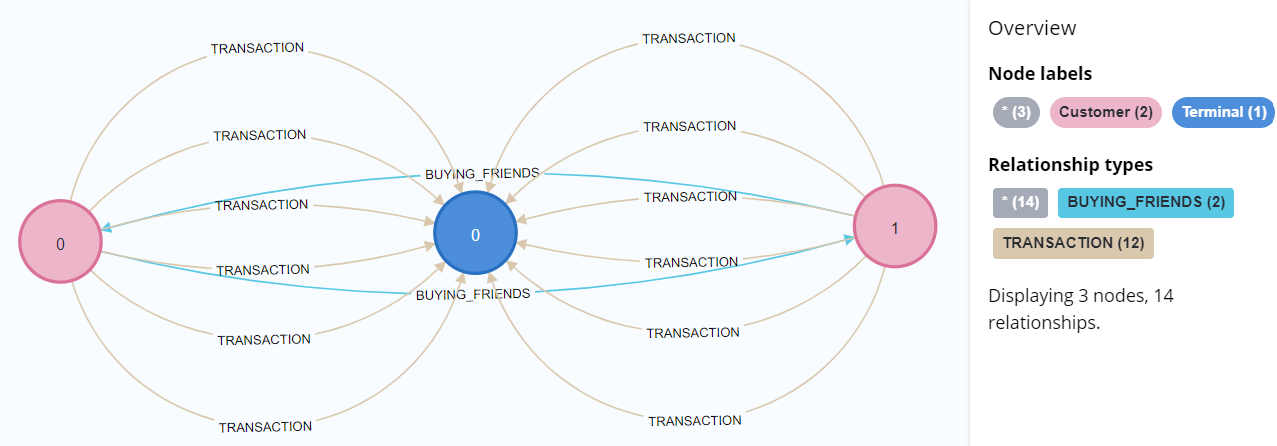
\includegraphics{images/buying-friends.png}
\caption{buying\_friends}
\end{figure}

    \hypertarget{query-e}{%
\subsubsection{Query (E)}\label{query-e}}

    \textbf{Query:} For each period of the day identify the number of
transactions that occurred in that period, and the average number of
fraudulent transactions.

\textbf{Assumptions:} In order to compute the average number of
fraudulent transactions, we use the \texttt{tx\_fraud} property as a
reference.

    \begin{tcolorbox}[breakable, size=fbox, boxrule=1pt, pad at break*=1mm,colback=cellbackground, colframe=cellborder]
\prompt{In}{incolor}{54}{\boxspacing}
\begin{Verbatim}[commandchars=\\\{\}]
\PY{n}{query\PYZus{}E} \PY{o}{=} \PY{l+s+s1}{\PYZsq{}\PYZsq{}\PYZsq{}}
\PY{l+s+s1}{    MATCH (:Customer)\PYZhy{}[t:TRANSACTION]\PYZhy{}(:Terminal)}
\PY{l+s+s1}{    RETURN}
\PY{l+s+s1}{        t.period\PYZus{}of\PYZus{}day AS period\PYZus{}of\PYZus{}day,}
\PY{l+s+s1}{        count(t) AS transaction\PYZus{}count,}
\PY{l+s+s1}{        round(avg(t.tx\PYZus{}fraud), 3) AS fraud\PYZus{}percentage}
\PY{l+s+s1}{\PYZsq{}\PYZsq{}\PYZsq{}}
\end{Verbatim}
\end{tcolorbox}

    \begin{tcolorbox}[breakable, size=fbox, boxrule=1pt, pad at break*=1mm,colback=cellbackground, colframe=cellborder]
\prompt{In}{incolor}{55}{\boxspacing}
\begin{Verbatim}[commandchars=\\\{\}]
\PY{n}{df\PYZus{}E\PYZus{}50} \PY{o}{=} \PY{n}{db}\PY{o}{.}\PY{n}{read\PYZus{}from\PYZus{}db}\PY{p}{(}\PY{n}{query\PYZus{}E}\PY{p}{,} \PY{n}{query\PYZus{}name}\PY{o}{=}\PY{l+s+s1}{\PYZsq{}}\PY{l+s+s1}{query\PYZus{}E}\PY{l+s+s1}{\PYZsq{}}\PY{p}{,} \PY{n}{database}\PY{o}{=}\PY{l+s+s1}{\PYZsq{}}\PY{l+s+s1}{TG50}\PY{l+s+s1}{\PYZsq{}}\PY{p}{)}
\PY{n}{df\PYZus{}E\PYZus{}100} \PY{o}{=} \PY{n}{db}\PY{o}{.}\PY{n}{read\PYZus{}from\PYZus{}db}\PY{p}{(}\PY{n}{query\PYZus{}E}\PY{p}{,} \PY{n}{query\PYZus{}name}\PY{o}{=}\PY{l+s+s1}{\PYZsq{}}\PY{l+s+s1}{query\PYZus{}E}\PY{l+s+s1}{\PYZsq{}}\PY{p}{,} \PY{n}{database}\PY{o}{=}\PY{l+s+s1}{\PYZsq{}}\PY{l+s+s1}{TG100}\PY{l+s+s1}{\PYZsq{}}\PY{p}{)}
\PY{n}{df\PYZus{}E\PYZus{}200} \PY{o}{=} \PY{n}{db}\PY{o}{.}\PY{n}{read\PYZus{}from\PYZus{}db}\PY{p}{(}\PY{n}{query\PYZus{}E}\PY{p}{,} \PY{n}{query\PYZus{}name}\PY{o}{=}\PY{l+s+s1}{\PYZsq{}}\PY{l+s+s1}{query\PYZus{}E}\PY{l+s+s1}{\PYZsq{}}\PY{p}{,} \PY{n}{database}\PY{o}{=}\PY{l+s+s1}{\PYZsq{}}\PY{l+s+s1}{TG200}\PY{l+s+s1}{\PYZsq{}}\PY{p}{)}
\end{Verbatim}
\end{tcolorbox}

    \begin{Verbatim}[commandchars=\\\{\}]
The query returned 4 records in 0.824 s.
The query returned 4 records in 0.897 s.
The query returned 4 records in 1.655 s.
    \end{Verbatim}

    The table below demonstrates the fraud percentage for each period of the
day in the \texttt{TG200} database.

    \begin{tcolorbox}[breakable, size=fbox, boxrule=1pt, pad at break*=1mm,colback=cellbackground, colframe=cellborder]
\prompt{In}{incolor}{56}{\boxspacing}
\begin{Verbatim}[commandchars=\\\{\}]
\PY{n}{df\PYZus{}E\PYZus{}200}\PY{o}{.}\PY{n}{rename}\PY{p}{(}\PY{n}{columns}\PY{o}{=}\PY{k}{lambda} \PY{n}{x}\PY{p}{:} \PY{n}{x}\PY{o}{.}\PY{n}{replace}\PY{p}{(}\PY{l+s+s1}{\PYZsq{}}\PY{l+s+s1}{\PYZus{}}\PY{l+s+s1}{\PYZsq{}}\PY{p}{,} \PY{l+s+s1}{\PYZsq{}}\PY{l+s+s1}{\PYZhy{}}\PY{l+s+s1}{\PYZsq{}}\PY{p}{)}\PY{p}{)}
\end{Verbatim}
\end{tcolorbox}
 
            
\prompt{Out}{outcolor}{56}{}
    
    \begin{center}
\begin{tabular}{llrr}
\toprule
 & period-of-day & transaction-count & fraud-percentage \\
\midrule
0 & evening & 145601 & 0.042000 \\
1 & afternoon & 420391 & 0.041000 \\
2 & morning & 421718 & 0.041000 \\
3 & night & 145280 & 0.041000 \\
\bottomrule
\end{tabular}

\end{center}

    

    \hypertarget{execution-times}{%
\subsection{Execution Times}\label{execution-times}}

    The execution times taken to perform each of the queries mentioned above
on all the graph databases are summarized below (in seconds):

    \begin{tcolorbox}[breakable, size=fbox, boxrule=1pt, pad at break*=1mm,colback=cellbackground, colframe=cellborder]
\prompt{In}{incolor}{57}{\boxspacing}
\begin{Verbatim}[commandchars=\\\{\}]
\PY{n}{df\PYZus{}exec\PYZus{}times} \PY{o}{=} \PY{n}{pd}\PY{o}{.}\PY{n}{DataFrame}\PY{p}{(}\PY{n}{db}\PY{o}{.}\PY{n}{read\PYZus{}execution\PYZus{}times}\PY{p}{)}
\PY{n}{df\PYZus{}exec\PYZus{}times}\PY{o}{.}\PY{n}{rename}\PY{p}{(}\PY{n}{columns}\PY{o}{=}\PY{k}{lambda} \PY{n}{x}\PY{p}{:} \PY{n}{x}\PY{o}{.}\PY{n}{replace}\PY{p}{(}\PY{l+s+s1}{\PYZsq{}}\PY{l+s+s1}{\PYZus{}}\PY{l+s+s1}{\PYZsq{}}\PY{p}{,} \PY{l+s+s1}{\PYZsq{}}\PY{l+s+s1}{\PYZhy{}}\PY{l+s+s1}{\PYZsq{}}\PY{p}{)}\PY{p}{)}
\end{Verbatim}
\end{tcolorbox}
 
            
\prompt{Out}{outcolor}{57}{}
    
    \begin{center}
\begin{tabular}{lrrrrrr}
\toprule
 & query-A & query-B & query-C & query-D1 & query-D2 & query-E \\
\midrule
TG50 & 4.240000 & 1.211000 & 0.957000 & 8.120000 & 3.292000 & 0.824000 \\
TG100 & 2.639000 & 1.688000 & 1.016000 & 10.959000 & 13.130000 & 0.897000 \\
TG200 & 3.098000 & 2.821000 & 1.768000 & 21.910000 & 189.534000 & 1.655000 \\
\bottomrule
\end{tabular}

\end{center}

    

    \begin{tcolorbox}[breakable, size=fbox, boxrule=1pt, pad at break*=1mm,colback=cellbackground, colframe=cellborder]
\prompt{In}{incolor}{58}{\boxspacing}
\begin{Verbatim}[commandchars=\\\{\}]
\PY{n}{fig}\PY{p}{,} \PY{n}{ax} \PY{o}{=} \PY{n}{plt}\PY{o}{.}\PY{n}{subplots}\PY{p}{(}\PY{n}{figsize}\PY{o}{=}\PY{p}{(}\PY{l+m+mi}{8}\PY{p}{,} \PY{l+m+mi}{4}\PY{p}{)}\PY{p}{)}
\PY{n}{sns}\PY{o}{.}\PY{n}{lineplot}\PY{p}{(}\PY{n}{data}\PY{o}{=}\PY{n}{df\PYZus{}exec\PYZus{}times}\PY{p}{,} \PY{n}{ax}\PY{o}{=}\PY{n}{ax}\PY{p}{,} \PY{n}{palette}\PY{o}{=}\PY{l+s+s1}{\PYZsq{}}\PY{l+s+s1}{Set2}\PY{l+s+s1}{\PYZsq{}}\PY{p}{)}
\PY{n}{ax}\PY{o}{.}\PY{n}{set\PYZus{}title}\PY{p}{(}\PY{l+s+s1}{\PYZsq{}}\PY{l+s+s1}{Execution Times for Different Queries in each Database}\PY{l+s+s1}{\PYZsq{}}\PY{p}{,} \PY{n}{fontsize}\PY{o}{=}\PY{l+m+mi}{14}\PY{p}{)}
\PY{n}{\PYZus{}} \PY{o}{=} \PY{n}{ax}\PY{o}{.}\PY{n}{set}\PY{p}{(}\PY{n}{xlabel}\PY{o}{=}\PY{l+s+s1}{\PYZsq{}}\PY{l+s+s1}{Graph Database Name}\PY{l+s+s1}{\PYZsq{}}\PY{p}{,} \PY{n}{ylabel}\PY{o}{=}\PY{l+s+s1}{\PYZsq{}}\PY{l+s+s1}{Time (s)}\PY{l+s+s1}{\PYZsq{}}\PY{p}{)}
\end{Verbatim}
\end{tcolorbox}

    \begin{center}
    \adjustimage{max size={0.9\linewidth}{0.9\paperheight}}{images/outputs/output_123_0.png}
    \end{center}
    { \hspace*{\fill} \\}
